\documentclass[11pt]{article}

\usepackage[]{graphics}
\usepackage{graphicx} % Required for inserting images
\usepackage{natbib}
\usepackage[margin=2cm]{geometry}
\usepackage{todonotes}
\usepackage[colorlinks=true, allcolors=black]{hyperref}
\usepackage{float}
\usepackage{tabularx}
\usepackage{subcaption}
\usepackage{array}
\usepackage{longtable}
\usepackage{ltablex} % This helps in handling long tables

%opening
\title{Developing an Intelligent Chatbot: the First Interim Report}
% \todo{Add everyones student number to author}
\author{Group 01: Cemal Ata Uzgoren (100447097), Joshua Newton (100401106) and Aman Seth (100442755)}


\begin{document}

\maketitle

\tableofcontents
\newpage

\begin{abstract}
The goal of this project is to create a chatbot that helps users by using natural language processing (NLP). A chatbot is an automated dialogue system that uses natural language processing (NLP) to analyse user inquiries and provide appropriate responses %\cite{chatbot_nlp}
. In this project, we aim to develop a user service chatbot that can converse with users and help them in precisely three scenarios: locating the best train ticket in the United Kingdom; predicting delays between train stations starting from London and going all the way to Norwich; and offering backup plans in case of blockages on the Great Eastern Tracks in Greater Anglia between Colchester and Norwich. Simple and complex user inquiries can be entered into this chatbot, which will then process them, categorise them into one of the pre-existing labels, and provide related responses. The chatBot is based on machine learning (ML) models that is built using Scikit-learn, spaCy pre-trained models for NLP, along with NLTK (Natural  Language  Tool  Kit) and other in-built python libraries. 

\end{abstract}

\section{Introduction}
This report will describe, outline and display the efforts made towards creating an autonomous conversational agent (chatbot) to interact with a human user. The primary purpose includes searching the internet for cheap train tickets between two destinations and present the findings to the user to for procurement. This objective should be achieved through a short series of dialogue interactions. The second motive this chatbot aims to realise is the improvement to customer service through conversation. There is no limitation to the depth of assistance the chatbot can provide; a regression model to predict the arrival time at a final station of a journey was designed and implemented. Lastly, the chatbot must have the ability to provide train operators with assistance when dealing with contingencies through several suggested resolution actions. This is achieved by employing a knowledge base (KB) which includes information regarding possible contingencies and regulation documents with actions within accordance.



% (Brief introduction to the coursework. 
% You don't have to write much.  
% You may introduce a bit on chatbot in general if like, and why an intelligent chatbot is useful using the subsections headings if you wish.)  

\subsection{Background and Motivation}
Chatbots are useful tools for improving efficiency and reducing the human labour during tedious tasks. Chatbots in their infancy used predefined rules to converse with humans which led to considerable limitations in communication. However, the succeeding chat-bots utilised machine learning (ML) and natural language processing (NLP) to analyse and respond intelligently with context and nuance to the users input. Section \ref{sec: related works} describes the current standard of chatbots which are free to acquire and use. At present no commercially available chatbot hold the ability to confidently check live train times and prices or accurately predict delayed arrival times. The absence of these abilities is the motivation behind the project with the objective outlined in Section \ref{Sec: Aim and Objs}.


% A bit background information on chatbot in general and the coursework specification \citep{AI2018CW}.

\subsection{Aim and Objectives of this coursework}\label{Sec: Aim and Objs}
% You may rephrase the the aim and objectives from your point of view.
% Due to the limited access to train times and tickets we are poised with the task of: \begin{enumerate}
To successfully realise this project and develop a sufficient working chatbot, the following objectives must be met and accomplished: 
\begin{enumerate}
    \item Create a conversational agent
        \begin{enumerate}
            \item Create code to clean and deconstruct a users input to a manageable format
            \item Create a NLP mechanism to determine the users intention of their input 
            \item Create an interactive Graphical User Interface (GUI) for better experience
        \end{enumerate}

    \item Scrape train time service websites for live train times and prices
        \begin{enumerate}
            \item Accumulate a minimum of 5 online services or websites that can produce accurate live train times and prices
            \item Extract the relevant information into a sufficient data structure
        \end{enumerate}

    \item Display and converse the data collected to the user in a understandable manner
        \begin{enumerate}
            \item Displays the relevant information i.e. website name, fare amount and cheapest fare clickable link. 
        \end{enumerate}

    \item Deploy a deep learning regression network to predict a delay train line's arrival and departure
        \begin{enumerate}
            \item Collect dataset of train journeys from Norwich to London Liverpool Street
            \item Preprocess the data for optimal utilisation when using neural network models
            \item Develop a network model which will efficiently output a numeric value based on the users input
            \item Measure and refine the model until a satisfactory quality has been achieved
            \item Deploy the model using the chat-bot
        \end{enumerate}

    \item Create rule engine (RE) to provide contingency plans
        \begin{enumerate}
            \item Implement NLP technique to extract locations and blockage type from the staff user input. 
            \item The train stations can only be between Colchester and Norwich on Great Eastern Track in Greater Anglia.
            \item Create Rule Engine (RE) to provide alternate plans / routes to the train station staff based on the blockage type and stations provided.
        \end{enumerate}
\end{enumerate}

\subsection{Difficulties and Risks}
This project includes several inherent factors which need to be considered to avoid unethical practises and application restrictions. Firstly, a restriction against the use of paid APIs was established. During the attempted exploration and extraction of data, a large quantity of websites offered access to their data through their API after a paid transaction. The choice to circumvent this option avoid unwanted financial burden and mitigates any economic advantage against colleagues attempting the same project.\vspace{0.5cm}

\noindent
Moreover, web scraping is a topic of ethical consideration and requires a thorough evaluation before commencing an automated scraping script. Due to moral concerns, caution is needed to avoid overloading a website with too many requests in a short space of time. Failure to acknowledge these concerns could overload the server hosting the website, which as a result, could suffer from an overall loss of speed. In an extreme case this can be considered a denial-of-service (DoS) attack. It is common practise to deploy anti-scraping tools on websites which require the user to pass a CAPTCHA before accessing the data. Failure to pass the CAPTCHA will temporarily and on occasion permanently revoke the user access the website.\vspace{0.5cm}

\noindent
Furthermore, online websites can contain personal information that should be avoided by a scraping tool indefinitely. The nature of the data and websites should mitigate any personal information, however caution will be practised to ensure no personal data is extracted. The deployment of artificial ``user-agents'' to access Chrome web browser via Selenium has shown great promise as an option to avoid an accidental security breach of the website and as a result the chat-bot is blocked from said website. However, implementing web scraping scripts employing Selenium requires prior knowledge regarding accessing web elements and locators. Should the website be composed of React element, the challenge of creating dynamic code which searches and extract specific elements becomes too large to become viable. Furthermore, a lot of websites constantly update their locators and web elements, particularly when new features are being deployed as software patches or builds. This periodic shift necessitates a time commitment to maintain a close eye on the automation scripts created to extract data. Because web scraping scripts may begin to malfunction if the locators are altered, resulting in unexpected results displayed on the chatbot's graphical user interface.
 \vspace{0.5cm}

\noindent
The NLP models used in this project which are outlines in Section \ref{Sec: Methods/NLP} demonstrated considerable difficulty in determining small or all UK cities. Hence, the objective to extract locations from the sentences became a largely challenging aspect of this project. In addition to the cities, the indicated date and time were difficult to extract because the pre-trained spaCy models that are now in use are not strong enough to retrieve the information from a lengthy or intricate user input. Therefore, it was necessary to find alternative methods in order to complete the necessary chatbot tasks. \vspace{0.5cm}

\subsection{Work Plan}
The following section will outline what each member's efforts have been focused over the duration of the project.
\subsubsection{Cemal Ata Uzgoren}
\begin{itemize}
    \item Took the poston as team leader
    \item Led the design and development of the GUI for the chatbot
    \item Led the integrity issues handling across the all three NLP tasks (Task A, Task B, Task C)
\end{itemize}
\subsubsection{Aman Seth}
\begin{itemize}
    \item Implemented multiprocessing among six scraper scripts resulting in reduced time consumption in fetching and displaying cheapest fare results on GUI.
    \item Led the NLP implementation at the backend of the chatbot graphical user interface for all three tasks (Task A, Task B, Task C)
    \item Led the embedding of the regression model into the conversational script
    
\end{itemize}
% Aman seth took the lead on embedding the regression model developed into the conversional script.
\subsubsection{Josh Newton}
% The efforts made by Josh included:
\begin{itemize}
    \item Created initial web scraping scripts which included the a method using either the Selenium library or sending a prefilled payload to the service
    \item Led the processing and exploration of the dataset provided for training a regression model to predict the arrival time at Norwich during a journey departing from London Liverpool Street
    \item Led the evaluation of multiple models to conclude the most efficient and practical model to implement.
\end{itemize} 

\subsubsection{Ganttchart}
The following figure displays the planned and executed timeline of events required to complete the aims outlined in Section \ref{Sec: Aim and Objs}.
\begin{figure}[!htbp]
    \centering
    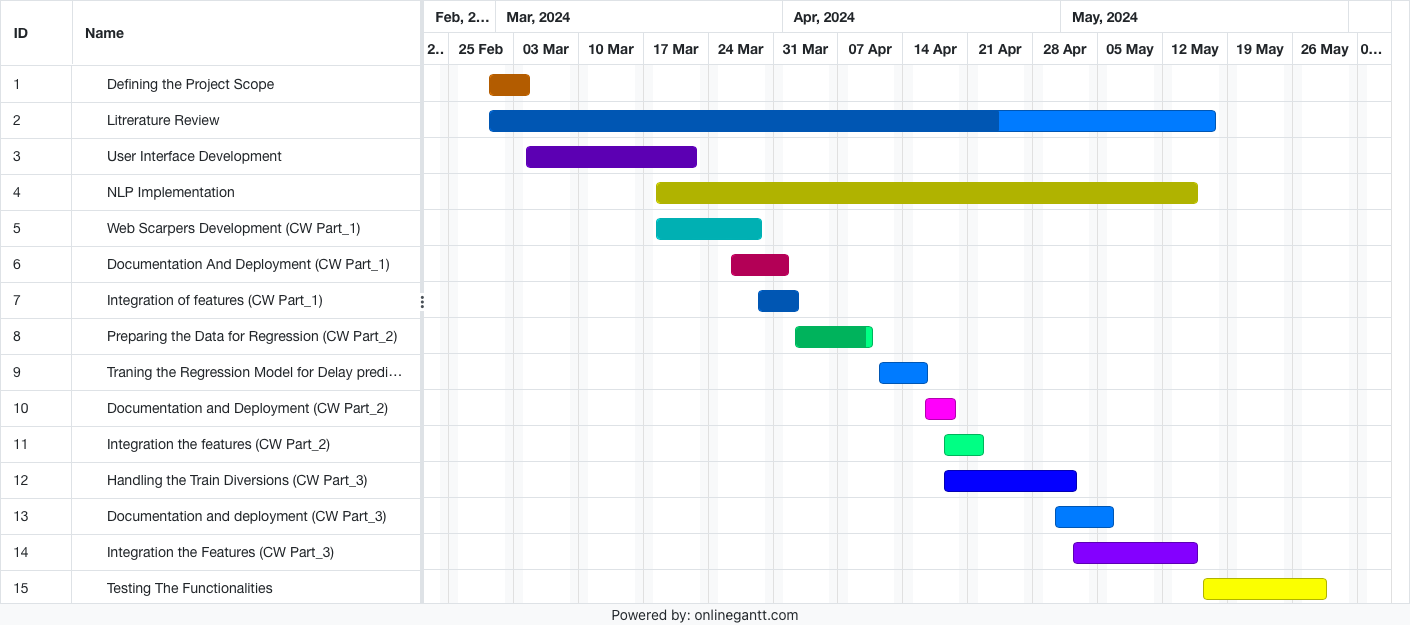
\includegraphics[width=\linewidth]{Diagrams/gant_chart.png}
    \caption{Gantt Chart displaying the execution timeline of tasks}
    \label{Fig: Gantt Chart}
\end{figure}

\section{Analysis of Related Work}\label{sec: related works}
This section will outline two examples of large language models (LLM) currently available for free and evaluate their performance with regards with the tasks relevant to this project. These include:
\begin{enumerate}
    \item Accurately searching the live arrival and departure of train times
    \item Offering the ability to provide the user with a URL link to purchase tickets extracted
    \item Predicting arrival train times when a train is delayed at a specific station during a journey
    \item Advising on the correct protocol when faced with contingencies
\end{enumerate}
\subsection{Microsoft Bing Co-Pilot}\label{Sec: Review Bing co-pilot}
The Microsoft Bing co-pilot is currently developed using the GPT-4.0 LLM manufactured by OpenAI \citep{bing-gpt4}. Unlike the Chat-GPT LLM, Bing co-pilot has the ability to extract information from the internet and utilise it in a conversional response. Due to this unique ability, it has become a powerful search engine alternative. The following sections will outline Bing co-pilot's ability to complete the tasks outlined in Section \ref{Sec: Aim and Objs}.

\subsubsection{Ability To Extract Live Train Ticket Prices}
This model demonstrates great ability for conversation however the main objective to achieve is to search and extract live train times of a given journey. When the model is prompted with the request ``find me the cheapest train ticket from London Liverpool Street to Norwich?'' it returned a vague response with no exact value or information. Figure \ref{Fig: example of bing co-pilot} demonstrates the response given which states a ``starting price of £10'' for the journey and also includes hyper links to online services to purchases train tickets.\vspace{0.5cm}

\noindent
Upon further inspection the quote of a ``£10 stating price'' was extracted from an online advertisements created by Trainline. A second attempt to request train tickets was explored with the following prompt ``Please can you find me the cheapest train ticket from London Liverpool Street to Norwich for Monday 20th at 12:00?''. Figure \ref{Fig: example of bing co-pilot revised} demonstrates a similar result to the previous prompt with a quoted starting price of £10. The hyperlink provided points to the TrainLine online service, the service displays a month calendar with the cheapest available ticket per day. Figure \ref{Fig: train-line booking results from bing} shows three days which match the quote of ``£10'' for the the cheapest ticket. Unfortunately, this response and suggested price is inaccurate as it is for days Wednesday 8th, Friday 7th and Saturday 8th, not Monday 20th as requested in the prompt. Moreover, accessing the particular date which quotes tickets in access of £10 is vacant of such prices. This leads to the assumption a singular ticket could cost £10 but would be at less that desirable off-peak times.

\subsubsection{Ability to Predict Train Delays}\label{Sec: Co-pilot delay prediction}
As per the secondary task described in Section \ref{Sec: Aim and Objs}, the LLM was prompted to predict the delayed arrival of a train journey between London Liverpool Street and Norwich when delayed at Ipswich. The following prompt ``I am currently on a train as Ipswitch during a journey from London Liverpool Street to Norwich. I left London at 12:00, the train was planned to depart from Ipswich at 13:07 but we are now departing at 13:15. What time would I arrive at Norwich?'' was given. The response was an inaccurate attempt as the predicted arrival time at Norwich was 14:56 when the true planned arrival time was 13:46. %As the prompted departure time from Ipswich was 8 minutes delayed which led the predicted arrival time to be one 1 hour and 10 minutes past the planned arrival time at Norwich, 
Figure \ref{Fig: bing copilot delay response} shows the response in full. Using our regression model to predict the arrival time using this scenario, the predicated arrival time was ``13:52'' which was 6 minutes later than the planned time. 

\subsubsection{Ability to handle and advise contingencies}\label{Sec: co-pilot contingencies}
As per the final task, the chatbot should be able to accurately advise a staff member on the protocol when faced with a contingency. The scenario referenced when interacting with the chat bot is a ``Full Line Blockage Between Ipswich and Stowmarket''. The prompt used was ``I am a train conductor on a train between Ipswich and Stowmarket. Unfortunately there is a full line blockage contingency. What should we do?''. Figure \ref{Fig: bing copilot contingency} shows the response, review of the response shows general safety advisory steps such as ensuring passenger safety, contacting and communicating with the rail control centre to report the blockage. This advice can be acceptable but shows no specific form of action.

\subsubsection{Conclusion}
The model can extract inaccurate information which appears to be a extracts from online advertisements and is dissimilar to the requirements found in the prompt. When asked to predict the delayed arrival at a station it gave an accurate description of the journey distance and travelling time but in despite of this, it gave an inaccurate arrival time. Overall the model shows potential for achieving the desired results. However due to the limitations of being a ``smart'' search engine, it relies on the collected internet sources to be accurate. %The LLM itself is unable to competently achieve the aims without the source material being accurate first.
With this key information the model cannot be confidently used to acquire train tickets or predict the delayed arrival times. When asked to advise on handling contingencies the model gave general advice without any specific instructions. The same prompt was given to our model which returned detailed instructions as shown in Figure \ref{Fig: Our-bot contingency}. A conclusion was drawn that within the given restrictions and goals, our chatbot was superior.


\subsection{Phi-3-mini}
The Microsoft developed MML Phi-3-mini boasts a moderate 3.8 billion parameters which were trained on 3.3 trillion tokens. It uses a transformer decoder architecture and limits itself with a default context length of 4$K$. However, with the introduction of LongRope, this limit extends to 128$K$, this extended model is named Phi-3-mini-128k. %It is currently open source and built on top of the Llama-2 family and uses the same tokeniser with vocabulary size of 32064. The model utilises the improvements from using the Tiktoken tokeniser with a vocabulary size of 100352. The results of this are... TBF As the model can be quantised to 4-bits, the required memory for the model to efficiently operate is $≈$ 1.8GB.
\subsubsection{Ability To Extract Live Train Ticket Prices}
When the model is prompted to fetch and present live train times, it will notify the user that the model is unable to get these values. Further testing shows that the model does not have access to the internet and thus live data. Figure \ref{Fig: Phi-3-mini train times} shows the response of the model. With this information no further testing was given.

\subsubsection{Ability to Predict Train Delays}
Similar to Section \ref{Sec: Co-pilot delay prediction} the chatbot was asked ``I am currently on a train as Ipswitch during a journey from London Liverpool Street to Norwich. I left London at 12:00, the train was planned to depart from Ipswich at 13:07 but we are now departing at 13:15. What time would I arrive at Norwich?''. The response shown in Figure \ref{Fig: Phi-3-mini dealy prediction} describes the train journey from Ipswich to Norwich as a 2 hour journey. However the TrainLine service, which was used as a reference, describes the journey as being 39 minutes as shown in Figure \ref{Fig: Trainline example LDN to NRW}. Both models have inaccurately estimated the journey time between these two stations.

\subsubsection{Ability to handle and advise contingencies}
Similar to Section \ref{Sec: co-pilot contingencies} the chatbot was asked how to handle a full Line Blockage Between Ipswich and Stowmarket. Figure \ref{Fig: Phi-3-mini contingency} shows the results which appears correlated to the response from Bing Co-Pilot. As the response is not detailed a conclusion that is was also insufficient was drawn, yielding our chatbot to be superior. 


\subsection{Evaluation and Comparison}
The reviewed chatbots appear to be subprior with general dialogue, specifically conversational responses. However, both models fall short of the tasks 2-5 outlined in \ref{Sec: Aim and Objs}. Solely based on these tasks, the aforementioned bots are not sufficient leaving our chatbot most acceptable.
\section{Methods, Tools and Frameworks}
% In this section, you should describe the methods, programming languages, packages, tools and framework you plan to use.
% for this report, you can list some you have identified and intend to use.
% No need to give any details.     

The primary programming languages used for this project are Python and JavaScript. \textit{PostgresDB} was initially considered for the KnowledgeBase, however the project has found sufficient success using local csv files as an alternative to databases.

\paragraph{Programming Languages:} Python \& JavaScript.
\paragraph{GUI development:} HTML \& CSS.
\paragraph{Packages:} NLP, NLTK locationtagger\citep{NLTK}, Spacy's ``en\_core\_web\_lg model''. For matching regex patterns: Selenium, requests, html-requests, BeautifulSoup, Minidom, lxml, urllib3 etc\dots %for web scraping mechanism. 
\paragraph{KnowledgeBase and Engine:} CSV \& JSON.\\
\noindent
\\Below is the in detail description of the tools and frameworks used for each component of the project:-
\subsection{Chatbot GUI}
\begin{itemize}
    \item Graphical User Interface: GUI development using JS, NodeJS, HTML, CSS.
    \item Voice Commands: Text-to-Speech \& Speech-To-Text recognition using APIs such as webkitSpeechRecognition, SpeechRecognition etc. 
\end{itemize}
\subsection{Web Scraping}
\begin{itemize}
    \item Selenium: This library was used to scrape data from the websites who doesn't provide any API to extract data in form of response.
    \item Requests: This module was used to extract data via HTTP/HTTPS requests.
    \item BeautifulSoup: This library was used to scrape websites HTML elements to fetch data.
\end{itemize}
\subsection{Chatbot Conversation - NLP}\label{Sec: Methods/NLP}
    \begin{itemize}
        \item Spacy: This library was used for natural language processing specifically for named-entity recognition (NER).
        \item Nltk: This toolkit was used along with spaCy for NLP.
        \item Fuzzywuzzy: This library was used to determine closes matches in the user input to extract relevant information.
        \item Experta: This library was used for building expert systems to provide suitable answers to the user.
    \end{itemize}
\subsection{Regression Model Prediction}
\paragraph{Models Utilised}
A variety of commonly implemented regression models were employed to predict the arrival at Norwich from the departure from London Liverpool Street. These models incline:
\begin{itemize}
    \item Multi Layer Perception (MLP) Regression: the sklearn.neural\_network library was used to build a simple MLP model \citep{scikit-learn}.
    \item K-Nearest Neighbors (KNN) Regression: the sklearn.neighbors library was used to build and tune a K-Nearest Neighbors model \citep{scikit-learn}.
    \item XGBoost (XGB) Regression: the XGBoost model from \cite{chen2016xgboost} was implemented.
    \item Random Forest (RF) Regression: the sklearn.ensemble library was used to build and tune a Random Forest model \citep{scikit-learn}.
    \item Linear Regression: the sklearn.linear\_model library was used to implement a Linear Regression model \citep{scikit-learn}.
    \item Huber Regressor: the sklearn.linear\_model library was used to implement a Huber Regressor model \citep{scikit-learn}.
    \item Lasso Regressor: the sklearn.linear\_model library was used to implement a Lasso Regressor model \citep{scikit-learn}.
    \item Stochastic Gradient Descent Regressor: the sklearn.linear\_model library was used to implement a Stochastic Gradient Descent Regression model \citep{scikit-learn}.
\end{itemize}

\paragraph{Metrics and performance evaluation}\label{Sec: Regression Metrics & performance}
During the training process each model was fitted to 80\% of the dataset while 20\% was employed as validation data. Each model will predict the arrival time at Norwich based on the values in the training dataset.

    \begin{itemize}
        \item NumPy: This was used for data manipulation and numerical calculate \citep{harris2020array}.
        \item Pandas: This was used for data storage inside dataframes along with dataframe manipulation tasks \citep{reback2020pandas}.
        \item sklearn: This library was used for data preprocessing and model metrics \citep{scikit-learn}.
        \item Seaborn and MatPlotlib: was used to generate visual representation of the data \citep{Waskom2021},\citep{Hunter:2007}.
    \end{itemize} 
 
\subsection{Development Framework}
The following sections outline and describe the current efforts and developments made towards achieving the aims and objectives described in Section \ref{Sec: Aim and Objs}.

\subsubsection{Flowchart}
Figure \ref{Fig: Flowchart} details a high-level flow chart of the chatbot when the user requests a train ticket. 

\subsubsection{Use Case and Sequence Diagrams}
Figure \ref{Fig: use case whole system} describes a use case diagram of the whole system. Also the general logic of the chatbot constructed by following the algorithms of the sequence diagrams which are stated in figure \ref{}, \ref{}, and \ref{} for each of the parts.

% \subsubsection{Sequence Diagrams}\label{Sec: Sequence Diagrams}
% The following sections describes the sequence diagrams for each mechanism the acheive the goals outlined in Section \ref{Sec: Aim and Objs}.
\section{Implementation}

\subsubsection{Web Scraping}
The model is developed to extract the required data from the following train booking websites:
\begin{enumerate}
    \item \href{https://www.lner.co.uk/}{LNER}
    \item \href{https://www.greateranglia.co.uk/}{Greater Anglia}
    \item \href{https://www.mytrainticket.co.uk/}{My Train Ticket}
    \item \href{https://www.nationalrail.co.uk/}{National Rail}
    \item \href{https://www.southernrailway.com/}{Southern Railways}
    \item \href{https://www.mytrainpal.com/}{Train Pal}
\end{enumerate}

The required information extracted are as follows:

\begin{itemize}
    \item Chepeast website name
    \item Fare amount
    \item Cheapest fare website link
\end{itemize} 

\subsubsection{Graphical User Interface Development}
The graphical user interface (GUI) is developed with text-to-speech and speech-to-text recognition feature embedded. The interface understands the voice commands given by user and displays on the UI. Based on the commands received, it attempts to fetch the result from the NLP and displays back on the screen. A spinner / loader is also implemented while the response is being fetched by chatbot for a reliable experience. Figure \ref{Fig: GUI Example} shows an example of the current GUI state.

\subsubsection{NLP Implementation}
The development of the natural language processing (NLP) behind the chatbot was made using a combination of SpaCy, NLTK (Natural Language Tool Kit), Scikit-learn and other in-built python libraries. The user input sentence was lemmatised first, meaning  linking similar meaning words as one word \cite{lemmatization}, then extracting the relevant details to fulfill the task and finally performing action as per the detected task and providing the appropriate response back to the user. \paragraph{Lemmatization:} The stop words were removed during the sentence cleaning process but leaving \textit{to} and \textit{from}. The intention behind leaving these two words were to figure out the origin / departing and arriving stations from the users input. \paragraph{Labels Creations \& Detection:} There were various different labels which were created as per the tasks which this chatbot should be able to perform. Some of the key labels are \textit{train}, \textit{location}, \textit{date}, \textit{time}, \textit{return}, \textit{delay}, \textit{contingency}, \textit{blockage}, \textit{assist}, \textit{help} etc. The sentences matched against these labels invoke their respective functionality functions to perform their tasks to achieve the end goal. \paragraph{Similarity Check:} The sanitised user input gets matched to the label which it belongs. The system calculate the similarity index via \textit{similarity()} which is an in-built function within spaCy python module. If the similarity matches with the minimum similarity defined threshold, it invokes a certain task as per the matched label. \paragraph{Stations Extraction: } It was observed that the spaCy and NLTK in-built functions could only fetch the renowned cities of the UK such as London, Birmingham, Manchester etc but they could not fetch small cities / stations such as Exeter, Norwich, Seven Kings etc. Hence they were not fully reliable and another approach had to be implemented. The \textit{stations.csv} containing all possible stations within the United Kingdom was used to match the stations against the user input. The already lemmatised user input which re-cleansed even more to shrink the user input as much as possible so that the match could have been easy. If there an exact match of the station in the user input to \textit{stations.csv}, the system would return the exact matching stations. Even the input has a partial match in case there is spelling mistake or there is a genuine partial matching for instance, if user enters London as input but London contains 10+ train stations such as London Piccadilly or London Liverpool Street etc, the system would return all the partially matched station asking the user to choose the precise ones. \paragraph{Date \& Time Extraction:} The time extraction was performed mainly using python regex matching. Since spaCy and NLTK libraries performed quite poorly in time extraction from a sanitised sentence, various regex matching were placed instead. \paragraph{Return Ticket Mechanism:} Return ticket functionality has been implemented in the first task of the chatbot that is to find the cheapest train fare within the UK. The chatbot asks the user once one-side train fare search is performed if the user wants to view cheapest return fares as well. The user may wish not to view return fares and simply quit the conversation. But NLP has been implemented if user wishes to view return fares too. Assuming the return would be within the same stations as one-way search, hence the chatbot would ask the user for only date and time of the return. Once the details are provided, the return fares are then searched and returned on the GUI. \paragraph{Delay Calculation Mechanism:} The delay calculation was implemented comprising of the details which are required from the user as input followed by invoking the saved ML model for predicted delay time calculation. The chatbot asks the user for the time of the last or current departed station, the name of the last or current departed station and lastly the time when the user departed from the origin station i.e by default London. Once all the details are received, the chatbot returns the predicted delay to reach to the destination i.e Norwich on it's user interface. \paragraph{Contingency Plans:} The NLP implemented behind the task of providing the contingency plans to the train station staff comprise of the details such has the name of the train stations on the Great Eastern Track in Greater Anglia facing the blockage and the type of the blockage i.e either \textit{Partial} or \textit{Full}. On receiving this information from the user, the alternate plans / routes are displayed on the chatbot GUI.

\subsubsection{Knowledge Base \& Inferring Engine}
The knowledge base used for this project are in the form of JSON files containing the rules for different types of intentions expressed by the user in it's input. The JSON contained the labels as the keys. The labels refer to the intention or the type of task requested by the user. Once the intention matches the label key, the responses stored as values against the keys in the JSON were inferred and returned to the user. 

\subsubsection{Regression Model}
The developments into the delayed arrival time predictive model was made using a combination of JuPyter Notebook and the later integration into the conversational Python script. The Notebook environment was chosen as an intuitive way to display and understand the data processing and model training. Once the model(s) were trained and saved to a recallable file, code to recall each file embedded into Python scripts then become the main executable location.

\paragraph{Data Types}\label{sec: Data Processing}
A detailed review of the data revealed that the majority of value types were string formats with 24-hour time values. Initially, there was a plan to encode each column containing string values using an array of methods including Binary Encoding, One Hot Encoding, Label Encoding, and Target Encoding. However, due to the complexity and quantity of unique values, encoding timestamp values proved inefficient. Instead, the Pandas library was utilised to convert the string value to datetime objects using the format Hour : Minute. Immutable or missing values are handled and replaced with a Not A Time (NaT) value.\vspace{0.5cm}

\noindent
The timecode objects were transformed to calculate the number of seconds since midnight. This calculation involves multiplying the hour component by 3600, the minute component by 60, and summing these products. The reason for using this method is that it provides a simpler normalisation process, simplifies calculations, and reduces dimensionality, which in turn can improve model performance. 

\paragraph{Encoding the tlp}\label{sec: Encoding the tlp}
As described in Table \ref{tab: Table of dataset column headers} the column ``tlp'' held the timing point locations for all stations of the journey. Examples of the values included: ``SHENFLD'', ``NRCHTPJ'', ``NRCH'' and ``TROWSEJ''. Due to the data only containing journeys between London Liverpool Street and Norwich, there were 34 unique values as described in Table \ref{tab: Table of dataset column headers}. Due to to considerably small quantity of values, the Label Encoder method is utilised as the encoder. Table \ref{tab:tpl encoding} showed the original ``tlp'' values and their corresponding encoded values.

\paragraph{Binary Valued Columns}
In addition to the encoding practices described Section \ref{sec: Encoding the tlp},it is important to note that while columns with binary values were encoded with either a ``1'', ``0''. These encoded representations did not feature in the final set of extracted features as they were deemed less effective for our predictive modelling objectives.

\paragraph{Feature Extraction}
The dataset comprised an extensive range of timestamps that incorporated predicted, estimated, planned, and actual times. Table \ref{tab: Table of dataset column headers} outlines the features paired with a description. The essential features necessary to predict arrival time at Norwich (NRW) during a journey from London Liverpool Street (LST), included the station's unique code, the departing time from LDN, departing time from each individual station and arrival time at NRW. As a result of adopting a simple feature set, there was an efficient systematic approach to handling missing values detailed in the following section.

\paragraph{Missing Values}\label{sec: missing values} The dataset contained an inherently large proportion of NaN values owing to a single time value being recoded at a singular point in time. To mitigate the issue of missing data, an systematic strategy was employed that involved the conditional imputation based on temporal availability. The process was structured hierarchically; firstly, the extraction of actual departure and arrival time instances were prioritised; however, when such records were unavailable, estimated values were introduced. Should the estimated values also be null, predicted values were employed as a final resort. As an additional method for dealing with missing information, passing times were occasionally used.
\section{Testing}
\subsection{Unit Testing}
As seen in Figure \ref{Fig: unit test results} a total of 23 unit tests were developed and implemented, these test can be split into three categorise: ``conversational functions'', ``scraping functions'' and ``contingency functions''. Table \ref{Tab: unit tests convo functions} shows the results of the conversational function tests. From these results we can see one failed case ``test\_lemmatise\_4'', the failure was a result of the lemmatise function not removing the ``@'' from the input string. Table \ref{tab: unit tests web scraping} show the results of each web scraping function implemented. From these results we can see 3 scraping scripts have failed, these failures can be a result of various errors. The suspected issues are: 
\begin{itemize}
    \item Blocked Selenium client from anti bot scripts
    \item Website HTML alterations which could break the Selenium object detection functions
\end{itemize}


\subsection{Integration Testing}

\begin{longtable}{|p{2cm}|p{4cm}|p{4cm}|p{4cm}|}
    \hline
    \textbf{Test ID} & \textbf{Integration point} & \textbf{Test Description} & \textbf{Expected result} \\
    \hline
    \endfirsthead
    \multicolumn{4}{c}%
    {\tablename\ \thetable\ \textit{}} \\
    \hline
    \textbf{Test ID} & \textbf{Integration point} & \textbf{Test Description} & \textbf{Expected result} \\
    \hline
    \endhead
    \hline \multicolumn{4}{|r|}{\textit{}} \\ \hline
    \endfoot
    \hline
    \endlastfoot
    
    P1 & Part 1 (Finding the cheapest fare) & Test the functionality of finding the cheapest fare. Start a conversation to provide the required information for ticket booking. & Chatbot returns the cheapest train ticket fare. \\
    \hline
    
    P2 & Part 2 (Delay Estimation) & Test delay estimation intelligence of the chatbot. Ask for the delayed train's information and get the predicted arriving time. & Chatbot estimates the delay correctly regarding to provided details. \\
    \hline
    
    P3 & Part 3 (Contingency recommendations) & Test the contingency function of the chatbot. Give a to get a contingency plan for that circumstance. & Chatbot provides appropriate probability recommendations according to predefined rules and regulations \\
    \hline
    
    TC1 & Part 1 and Part 2 & Initialise a conversation about fare search. After completing the train ticket search, ask for delay estimation. & Chatbot finds the cheapest fare and estimated the delay correctly without being influenced by each other. \\
    \hline
    
    TC2 & Part 2 and Part 3 & Start conversation for both part 2 and 3 respectively, and examine the results to make sure that the part 2 and 3 not effect each other. & Chatbot should perform the delay estimation and contingency plan recommendation correctly. \\
    \hline
    
    TC3 & Part 1 and Part 3 & Start conversation for both part 1 and 3 respectively, and examine the results to make sure that the part 1 and 3 not effect each other. &  Chatbot should perform the cheapest train fare search and delay estimation correctly. \\
    \hline
    
    TC4 & Contradictions & Test the contradiction feature that restricts the user switch to another subject while an ongoing conversation takes place about something else. & Chatbot displays a informative message which says to switch to another conversation either reset the current conversation or finalise it. \\
    \hline
    
    GUI & GUI Integration & Test the integration of the graphical user interface with all parts of the chatbot. Perform tasks related to ticket finding, delay estimation and contingency recommendation using the GUI. & GUI handles the conversation about all parts flawlessly and orients the user for next steps.  \\
    \hline
    \end{longtable}
    
% \subsection{System Testing} --> To be reviewed later 
\subsection{Usability Testing}
Two UEA students earning master's degrees, one in business and the other in computer science, conducted the usability testing demonstrated in the table below:-. 

\begin{longtable}{|c|p{3cm}|p{3cm}|p{3cm}|p{3cm}|p{3cm}|}
\hline
\textbf{ID} & \textbf{Description} & \textbf{Preconditions} & \textbf{Test Steps} & \textbf{Expected Results} & \textbf{Actual Results} \\ \hline
\endfirsthead
\hline
\textbf{ID} & \textbf{Description} & \textbf{Preconditions} & \textbf{Test Steps} & \textbf{Expected Results} & \textbf{Actual Results} \\ \hline
\endhead
TC01 & Find cheapest ticket for specified route, date and time & NodeJS server is up and running & 1. Enter departure and arrival locations \newline 2. Enter travel date and time \newline 3. Submit search query & Display cheapest ticket for the specified route, date and time & One-way ticket details displayed: Ticket price, Wesbite name and link  \\ \hline

TC02 & Find cheapest ticket for partially matched train stations & NodeJS server is up and running & 1. Enter partially matched departure and arrival stations & Display a list of partially matched available stations with input & Partially matched stations displayed asking user to give precise name choosing from the output \\ \hline

TC03 & Find cheapest ticket if time is not provided & NodeJS server is up and running & 1. Provide departing and arriving stations  \newline 2. Enter date but not time  \newline  3. Submit search query & Chatbot should ask the user to provide time & Time missing warning displayed on GUI \\ \hline

TC04 & Find cheapest ticket when stations are mis-spelled & NodeJS server is up and running & 1. Enter departure and arrival locations with misspelled words \newline 2. Submit search query & Display a list of partially matched available stations with input & Partially matched stations displayed asking user to give precise name choosing from the output \\ \hline

TC05 & Find cheapest return ticket & NodeJS server is up and running & 1. Enter departure and arrival locations \newline 2. Enter travel date and time \newline 3. Perform one-way ticket search \newline 4. Ask for return \newline 5. Submit search & Display return ticket cheapest fare details: Ticket price, website name and link & Return ticket details are displayed \\ \hline

TC06 & Find train delay by providing current or last departed station and time along with time from origin station & NodeJS server is up and running & 1. Enter current or previously departed station \newline 2. Enter departure time of previously departed station \newline 3. Enter departure time from origin station & Train delay to destination Norwich should be displayed & Delayed time is displayed on GUI \\ \hline

TC07 & Find train delay without providing departed time of origin station & NodeJS server is up and running & 1. Enter current or previously departed station \newline 2. Enter departure time of previously departed station \newline 3. Click submit button & Chatbot should ask the user to enter the departed time from origin station & Departed time from origin missing warning is displayed on GUI \\ \hline

TC08 & Find train delay of an unknown station & NodeJS server is up and running & 1. Enter current or previously departed station which is not betweeen london and norwich \newline 2. Click submit button & Chatbot should try partial matching and display warning message of station not found & Station not found message is displayed \\ \hline

TC09 & Find contingency plans for partial or full link blockage for valid stations on great easter track & NodeJS server is up and running & 1. Enter blockage type as full or partial \newline 2. Enter train stations on great eastern track \newline 3. Click submit button & Contingency plans should be displayed as per the blockage and stations given & Contingency plans displayed accordingly \\ \hline

TC10 & Find contingency plans without providing the blockage type & NodeJS server is up and running & 1. Enter train stations on great eastern track \newline 3. Click submit button & Chatbot should ask the user to enter the blockage type providing a hint to choose either partial of full & Missing blockage type warning is displayed on GUI \\ \hline

\caption{Usability Test Cases}
\label{tab:usability_testing}
\end{longtable}
\section{Evaluation and Discussion}
% \subsection{Regression Models} This needs to be moved to a previous section where we outline the regression side
% A variety of different regression models were trained and validated on the data each performing to a degree of competence, however a large margin of accuracy can be discovered when comparing the models together.


\subsection{NLP}
The following sections outline the chatbot's performance in natural language understanding, response accuracy, user experience, and technical robustness. 
\subsubsection{Natural Language Understanding (NLU)}
\begin{itemize}
    \item \textbf{Intent Recognition:} The chatbot correctly identifies user intentions, such as searching for train tickets, specifying travel date and time, querying about prices or requesting delay information or requesting for contingency plans in case of partial or full line blockage.
    \item \textbf{Entitiy Recognition:} The chatbot accurately identifies key entities like locations (departure and arrival), dates, times, and ticket preferences (e.g., on-way or return), blockage type etc.
    \item \textbf{Context Handling:} The chatbot is effective in maintaining context over a multi-turn conversation and understanding follow-up queries.
\end{itemize} 

\subsubsection{Response Accuracy}
\begin{itemize}
    \item \textbf{Correctness:} The chatbot accurately provided the information of the cheapest train ticket, delayed time display or alternate routes as per contingency plans.
    \item \textbf{Relevance:} The chatbot's responses are appropriate as per user queries.
    \item \textbf{Completeness:} The chatbot responses are comprehensive, providing all necessary information to the user.
\end{itemize} 

\subsubsection{User Experience (UX)}
\begin{itemize}
    \item \textbf{Ease of Use:} As per the usability testing in \ref{tab:usability_testing} carried out by different UEA students, the feedback was positive about chatbot being easy to use.
    \item \textbf{Response Time:} The response time of the answer was fairly short. The multi-processing implemented which runs the scraper scripts asynchronously rather than in serier, saved a lot of response time.
    \item \textbf{User Satisfaction:} The overall response from both of the UEA students who carried usability testing was positive and satisfactory.
\end{itemize} 

\subsubsection{Technical Robustness}
\begin{itemize}
    \item \textbf{Reliability:} The developed chatbot have consistence performance with correct and appropriate responses.
    \item \textbf{Error Handling:} The chatbot is robust enough to handle conversations related to different tasks as well as if there are grammatical errors in the user's input or even there is partial information given.
    \item \textbf{Integration:} The integrity constraints were applied in the chatbot to prevent delivering invalid information to the users.
\end{itemize}


\subsection{Regression Models}
The sections below outline and describe the research efforts made into regression models and the performance metrics of each.
% \subsubsection{Multi-layer Perceptron (MLP) Regressor}
% A simple MLP model was integrated using the
\subsubsection{Multi-layer Perceptron (MLP) Regressor}
A Multi-layer Perceptron (MLP) model was implemented using both the Scikit and Keras libraries, however the results were considerably inaccurate when compared to other models. Table \ref{tab:model metrics} shows its inaccuracy. Due to the limited time and computational resources a hyper parameter tuning mechanism such as Gridsearch or RandomSearch was not implemented. Neither was an extensive training run executed. With these circumstances and results the MLP models were made redundant and not used in the final predictions.

\subsubsection{K Nearest Neighbors Regressor:} \label{Sec: KNN tuning}
The parameter which configured the number of neighbours of the K-Nearest Neighbors (KNN) regression model was manually tuned using a $for$ loop which iteratively increased the value of $k$ and scored the model accordingly using metrics outlines in Section \ref{Sec: Regression Metrics & performance}. Figure \ref{Fig: KNN K vs k} shows the iteration of $k$, the results of these $k$ values can be seen in Figures: \ref{Fig: KNN K vs MAE}, \ref{Fig: KNN K vs R^2}, \ref{Fig: KNN K vs RMSE}. From these results we can see minimal prediction accuracy improvement when $k > 30$, on the contrary we can see great improvements when $k$ is increased to 20. With these results in mind, a $k$ value of 50 was used to maximise potential accuracy as the trade off between prediction time per value of $k$ was minimal.

\subsubsection{Random Forest Regressor:}
The Random Forest (RF) regression model was built with near-default parameters. The only specific change made to the configuration of the model was the number of estimators. Similar to the manual tuning of the KNN model outlined in Section \ref{Sec: KNN tuning}, an iterative $for$ loop was employed to score the model per number of estimators. Figure \ref{Fig: RF nn vs nn} displays the number of estimators searched, an initial value of 5 was chosen with an iterative increase of 1 until a value of 10 was selected. Once the value of estimators reached 10, an incrementation of 5 was chosen instead to increase efficiency. Table \ref{tab: RF score per K} displays scores per value of $k$. Figures \ref{Fig: RF MSE vs nn}, \ref{Fig: RF r^2 vs nn}, \ref{Fig: RF RMSE vs nn} show the models performance per iteration. From these results we can see the performance peaked at an estimator value of 8.
-
\begin{table}[!htbp]
    \centering
    % \begin{tabular}{|c|c|c|c|}
    \begin{tabularx}{\textwidth}{XXXX}
    \hline
    n\_estimators & RMSE & MAE & R2 \\
    \hline
    5 & 1692.184531 & 322.930468 & 0.993185 \\
    6 & 1692.829572 & 322.482591 & 0.993180 \\
    7 & 1689.592844 & 322.124198 & 0.993206 \\
    \textbf{8} & \textbf{1683.224923} & \textbf{321.827668} & \textbf{0.993257} \\
    9 & 1682.711353 & 321.882941 & 0.993261 \\
    10 & 1686.329066 & 322.128959 & 0.993232 \\
    ... & ... & ... & ... \\
    100 & 1685.108628 & 322.103318 & 0.993242 \\
    \hline
    % \end{tabular}
    \end{tabularx}
    \caption{Performance results of the Random Forest Regression model}
    \label{tab: RF score per K}
\end{table}

\subsubsection{XGBoost Regression:}
Similar the to K Nearest Neighbors and Random Forest models, the XGBoost model was implemented with default parameters with iteratively increasing number of estimators. Table \ref{tab:XGBoost score per N_estimators} and Figure \ref{fig: XGBoost estimators vs results} show the performance of the model per number of estimators. From these results we can see a correlation between an increased value of estimators and the models improved performance.


\begin{table}[!htbp]
    \centering
    % \begin{tabular}{|c|c|c|c|}
    \begin{tabularx}{\textwidth}{XXXX}
    \hline
    \textbf{n\_estimators} & \textbf{RMSE} & \textbf{MAE} & \textbf{R2} \\
    \hline
    1 & 14423.881550 & 11689.875945 & 0.504871 \\
    2 & 10194.480707 & 8214.249700 & 0.752666 \\
    3 & 7270.192730 & 5782.620130 & 0.874210 \\
    4 & 5271.073107 & 4084.681260 & 0.933877 \\
    5 & 3932.805430 & 2900.675047 & 0.963191 \\
    ...&...&...&...\\
    % 6 & 3064.765834 & 2075.270793 & 0.977646 \\
    % 7 & 2530.248765 & 1506.208446 & 0.984764 \\
    % 8 & 2219.225104 & 1115.703541 & 0.988279 \\
    % 9 & 2047.260012 & 852.227672 & 0.990025 \\
    % 10 & 1955.658498 & 677.491905 & 0.990898 \\
    % 15 & 1861.595469 & 424.721672 & 0.991752 \\
    % 20 & 1848.114642 & 405.720689 & 0.991871 \\
    % 25 & 1833.428678 & 401.357044 & 0.992000 \\
    % 30 & 1814.992326 & 399.066723 & 0.992160 \\
    % 35 & 1801.847733 & 397.325036 & 0.992273 \\
    % 40 & 1783.585265 & 395.618465 & 0.992429 \\
    % 45 & 1775.365191 & 393.974004 & 0.992499 \\
    50 & 1770.881199 & 392.856774 & 0.992537 \\
    55 & 1766.922512 & 391.254378 & 0.992570 \\
    65 & 1752.241861 & 388.335768 & 0.992693 \\
    75 & 1740.280743 & 385.322977 & 0.992792 \\
    85 & 1733.922944 & 383.150441 & 0.992845 \\
    95 & \textbf{1728.680439} & \textbf{381.605032} & \textbf{0.992888} \\
    \hline
    % \end{tabular}
    \end{tabularx}
    \caption{Performance metrics for XGBoost regressor per value of n\_estimators}
    \label{tab:XGBoost score per N_estimators}
\end{table}

\subsubsection{Metrics and results:}\label{sec: Metrics and results}
Table \ref{tab:model metrics} and Figures \ref{Fig: all_MAE}-\ref{Fig: all_RMSE} outline each models performance using the metrics described in Section. For a secondary evaluation, previous journey arrival and departure times were extracted from an online resource \href{https://www.recenttraintimes.co.uk/}{``Recent Train Times''} to be used as new unseen data. Figure \ref{fig: real delayed train times} and \ref{fig: real on-time train times} are two examples of the ground truth values extracted from the online source. Figure \ref{fig: inline_Regression models prediction of arrival time at Norwich} and \ref{fig: Regression model predicted arrival time at Norwich from London Liverpool Street} show the highest attaining classifiers predictions of the arrival time at Norwich using the data extracted.

\begin{table}[!htbp]
    \centering
    \begin{tabularx}{\textwidth}{XXXXX}
    \hline
    \textbf{Model Name} & \textbf{R2 Score} & \textbf{Mean Absolute Error} & \textbf{Root Mean Squared Error} & \textbf{Mean Squared Error} \\ 
    \hline
    MLP Regressor & 0.45369 & 7876.414635 & 15151.049907 & 229554313.277678 \\
    KN Regressor & 0.992975 & 337.436982 & 1718.046845 & 2951684.960503 \\
    XGB Regressor & 0.992888 & 381.605032 & 1728.680439 & 2988336.06081 \\
    RandomForest & \textbf{0.993242} & \textbf{322.103318} & \textbf{1685.108628} & \textbf{2839591.088781} \\
    Linear Regression & 0.394573 & 8650.629986 & 15949.750001 & 254394525.082963 \\
    Huber Regressor & 0.222805 & 5853.991688 & 18071.2504 & 326570091.003966 \\
    Lasso & 0.394573 & 8650.630322 & 15949.749997 & 254394524.969961 \\
    \hline
    \end{tabularx}
    \caption{Each model paired with the metric results}
    \label{tab:model metrics}
\end{table}

\begin{figure}[!htbp]
    \centering
    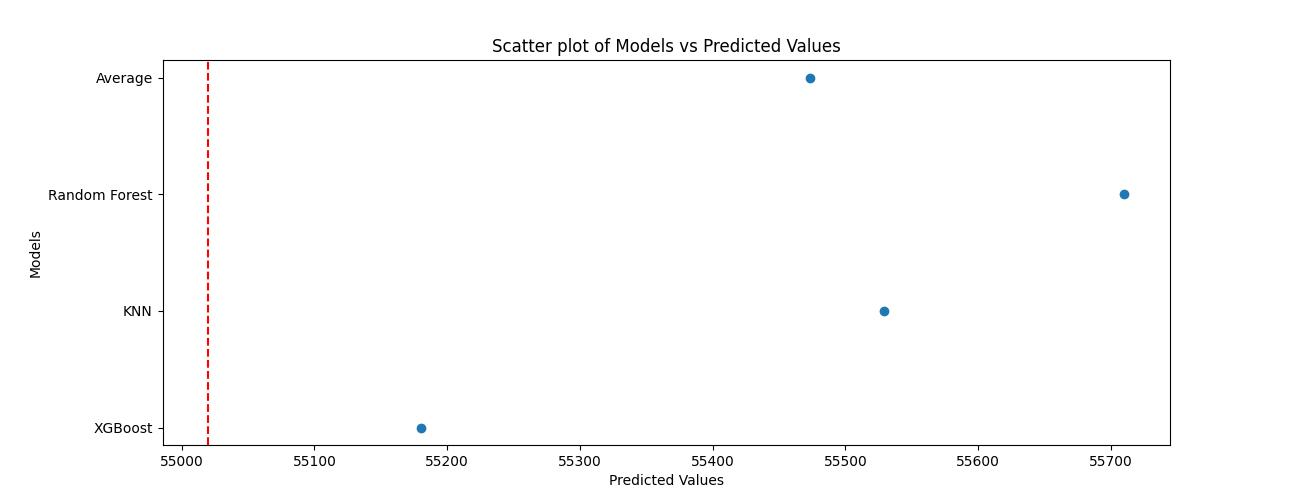
\includegraphics[width=\textwidth]{../regression_model/plots/Comparison/Scatter plot of Models vs Predicted Value 55020.jpeg}
    \caption[regression model predictions of previous journeys]{Regression models prediction of arrival time at Norwich from a departure from London Liverpool Station if delayed at Ipswich. The red dotted vertical line is ground truth.}
    \label{fig: inline_Regression models prediction of arrival time at Norwich}
\end{figure}

\subsubsection{Model Evaluation:}
From the results described in Section \ref{sec: Metrics and results} Random Forest, K Nearest Neighbors and XGBoost regressor models appear superior. However, as shown in Figures \ref{fig: inline_Regression models prediction of arrival time at Norwich} and \ref{fig: Regression model predicted arrival time at Norwich from London Liverpool Street} each model will have a degree of inaccuracy when making predictions, as a result no single model would be a better choice for deployment. An average value was instead used to capture the accuracy of each model.

\subsection{Areas for Improvement \& Future Enhancements}
The following sections describe the areas which could be subject to improvement should the project continue.
\subsubsection{Part A: Find cheapest train ticket}
\begin{itemize}
    \item In order to make the search for the cheapest train tickets more dynamic and accurate, the user should be allowed to enter other parameters, such as the number of adults and children and whether or not they have a rail card. If so, inquire about the kind of railcard, etc.
    \item The user should be able to request a return ticket all at once rather than having to wait for the one-way search to finish before responding to the chatbot's request to inquire whether they would also like a return ticket. The user may be able to save more money in this method.
    \item Even though multi-processing is used to run all of the scrapers asynchronously, the cheapest train fare search still takes a long time since the system needs time to render the response on the GUI. Redesigning the system could improve its performance.
\end{itemize}

\subsubsection{Part B: Find train delay}
\begin{itemize}
    \item In an attempt to improve the model's accuracy, more features could be introduced such as: days of the week, current weather at time of recording or public holiday occasion. One can assume these parameters should see considerable difference.
    \item The data provided was of decent size and quality, however an increased volume could be advantageous.
    \item At present the model will only predict the arrival time at Norwich station from London Liverpool Street. To improve upon this model, predictions of each mid-way station as well as predictions of other journeys should be possible.
\end{itemize}

\subsubsection{Part C: Fetch contingency plans}
\begin{itemize}
    \item Give the user the ability to request backup plans between any station on the Great Eastern track, not only the one between Colchester and Norwich.
    \item The system should be able to receive additional inputs based on various situations, such as whether the obstruction is the result of a natural disaster like heavy rain or flooding, and then return the contingency plans in accordance with those inputs in order to make the search more dynamic. Train services must be halted, etc., if the temperature rises beyond thirty degrees.
    \item It is also possible to give the backup plans due consideration. In the event of a blockage between two stations, the system ought to provide specific solutions, especially if it is close to midnight. A certain kind of response should be given if it's peak hour and so on.
\end{itemize}
\section{Conclusion}

This report outlines the efforts made towards creating an interactive chatbot with the ability to purchase online train tickets, predict time arrival time of delayed train and finally assist users when dealing with contingencies. The background and motivation includes the absence of chatbots with the ability to search for live train times. The extraction of train times includes several web scraping methods which require ethical consideration to avoid the misuse of the scripts.\vspace{0.5cm}

\noindent
At present the GUI has been developed and deployed and integrated into our chatbot which can respond to the user when asked for train tickets. The chatbot will respond to the user to collect the required information regarding the users journey. Several scraping scripts will be deployed to search a list of train ticket websites / services. The cheapest found ticket will be presented to the user with the respective URL to that ticket.\vspace{0.5cm}

\noindent
Development into regressive neural networks has yielded respectable results using the Keras library to build a draft LSTM model.\vspace{0.5cm}

\noindent
Future progress will include the refinement and completion of several regression models, with the inclusion of Integration into the chatbot script. The research into assisting the user with contingencies will be completed.


\bibliographystyle{agsm}
%\bibliographystyle{apalike}
% you should use your own bibtex file to replace the following example_ref bib file.
\bibliography{report_bib} 

\newpage
\appendix
\section{Appendix}
\subsection{Tables}

\begin{table}[!htbp]
    \centering
    \begin{tabular}{|l|r||l|r|}
    \hline
    \textbf{Original Value} & \textbf{Encoded Value} & \textbf{Original Value} & \textbf{Encoded Value} \\
    \hline
    BOWJ & 0 & ILFELEJ & 18 \\
    BROXBRN & 1 & ILFORD & 19 \\
    BRTWOOD & 2 & INGTSTL & 20 \\
    BTHNLGR & 3 & INGTSTN & 21 \\
    CHDWLHT & 4 & IPSWEPJ & 22 \\
    CHESHNT & 5 & IPSWESJ & 23 \\
    CHLMSFD & 6 & IPSWHJN & 24 \\
    CLCHSTR & 7 & IPSWICH & 25 \\
    DISS & 8 & KELVEDN & 26 \\
    FRSTGT & 9 & LIVST & 27 \\
    FRSTGTJ & 10 & MANNGTR & 28 \\
    GIDEAPK & 11 & MANRPK & 29 \\
    GIDEPKJ & 12 & MRKSTEY & 30 \\
    GODMAYS & 13 & MRYLAND & 31 \\
    HAGHLYJ & 14 & NEEDHAM & 32 \\
    HAKNYNM & 15 & NRCH & 33 \\
    HFLPEVL & 16 & NRCHTPJ & 34 \\
    HRLDWOD & 17 & ROMFORD & 35 \\
    SEVNSIS & 36 & STWMDGL & 39 \\
    SHENFLD & 37 & STWMRKT & 40 \\
    STFD & 38 & SVNKNGS & 41 \\
    TROWFLR & 42 & WARE & 45 \\
    TROWSEJ & 43 & WITHAME & 46 \\
    TRWSSBJ & 44 &  &  \\
    \hline
    \end{tabular}
    \caption{Mapping of original values to encoded values for the 'tpl' column (Part 1)}
    \label{tab:tpl encoding}
\end{table}

\begin{table}[!htbp]
    \centering
    \resizebox{\textwidth}{!}{%
    \begin{tabular}{|l|l|l|l|l|}
    \hline
    Column Name         &
    Data Type           &
    No. Unique Values   &
    Description         &
    Notes \\ \hline
    rid             & int64   & 660  & Train RTTI Train Identifier          & Unique code for train travel  \\ \hline
    tpl             & object  & 34   & TIPLOC (Timing point locations)      & Unique station code           \\ \hline
    pta             & object  & 285  & Planned Time of Arrival              & 24hr Time value               \\ \hline
    ptd             & object  & 282  & Planned Time of Departure            & 24hr Time value               \\ \hline
    wta             & object  & 384  & Working (staff) Time of Arrival      & 24hr Time value- with seconds \\ \hline
    wtp             & object  & 959  & Working Time of Passing              & 24hr Time value               \\ \hline
    wtd             & object  & 373  & Working Time of Departure            & 24hr Time value- with seconds \\ \hline
    arr\_et         & object  & 11   & Estimated Arrival Time               & 24hr Time value               \\ \hline
    arr\_wet        & object  & 9    & Working Estimated Time               & 24hr Time value               \\ \hline
    arr\_atRemoved  & object  & 2    & true if actual replaced by estimated & True / False                  \\ \hline
    pass\_et        & object  & 851  & Estimated Passing Time               & 24hr Time value               \\ \hline
    pass\_wet       & float64 & 1    & Working Estimated Time               & 24hr Time value               \\ \hline
    pass\_atRemoved & object  & 2    & true if actual replaced by estimated & True / False                  \\ \hline
    dep\_et         & object  & 14   & Estimated Departure                  & 24hr Time value               \\ \hline
    dep\_wet        & float64 & 1    & Working Estimated Time               & 24hr Time value               \\ \hline
    dep\_atRemoved  & object  & 2    & true if actual replaced by estimated & True / False                  \\ \hline
    arr\_at         & object  & 1048 & True time of arrival                 & 24hr Time value               \\ \hline
    pass\_at        & object  & 1121 & True time of train passing through   & 24hr Time value               \\ \hline
    dep\_at         & object  & 1008 & True time of train departure         & 24hr Time value               \\ \hline
    cr\_code        & float64 & 12   & Cancellation Reason Code             & Float value                   \\ \hline
    lr\_code        & float64 & 26   & Late Running Reason                  & Float Value                   \\ \hline
    \end{tabular}%
    }
    \caption{Table of dataset column headers and the number of unique values}
    \label{tab: Table of dataset column headers}
\end{table}

\begin{table}[!htbp]
    \centering
    \begin{tabular}{|l|r|r|l|l|}
    \hline
    \textbf{Index} & \textbf{arr\_at\_seconds\_since\_midnight} & \textbf{my\_prediction\_since\_midnight} & \textbf{arr\_at} & \textbf{my\_prediction} \\
    \hline
    9129 & 67440.0 & 67903.125000 & 18:44:00 & 18:51:43 \\
    9130 & 68040.0 & 68576.476562 & 18:54:00 & 19:02:56 \\
    9132 & 68760.0 & 68962.398438 & 19:06:00 & 19:09:22 \\
    9137 & 70140.0 & 70106.796875 & 19:29:00 & 19:28:26 \\
    9141 & 71340.0 & 71103.328125 & 19:49:00 & 19:45:03 \\
    ... & ... & ... & ... & ... \\
    27006 & 1620.0 & 1125.753540 & 00:27:00 & 00:18:45 \\
    27008 & 2220.0 & 2186.079834 & 00:37:00 & 00:36:26 \\
    27011 & 3000.0 & 2819.950684 & 00:50:00 & 00:46:59 \\
    27013 & 3720.0 & 3619.740723 & 01:02:00 & 01:00:19 \\
    27017 & 4860.0 & 4857.188477 & 01:21:00 & 01:20:57 \\
    \hline
    \end{tabular}
    \caption{Arrival predications made my draft RNN model}
    \label{tab:RNN prediction tables}
\end{table}

% unittests conversational chatbot
\begin{landscape}
    \begin{longtable}{|c|p{5cm}|p{5cm}|c|}
        \hline
        \textbf{Test\_ID} & \textbf{Input} & \textbf{Output} & \textbf{Pass/Fail} \\
        \hline
        \endfirsthead
        \multicolumn{4}{c}%
        {{\bfseries \tablename\ \thetable{} -- continued from previous page}} \\
        \hline
        \textbf{Test\_ID} & \textbf{Input} & \textbf{Output} & \textbf{Pass/Fail} \\
        \hline
        \endhead
        \hline \multicolumn{4}{|r|}{{Continued on next page}} \\ \hline
        \endfoot
        \hline
        \endlastfoot
        test\_convert\_date\_type & ``15th October'' & ``15/10/2024'' & Pass \\
        \hline
        test\_convert\_date\_value & ``15th October'' & d.type = string & Pass \\
        \hline
        test\_extract\_location\_multiple\_matches & ``Find me the cheapest train ticket from London Liverpool Street station to Norwich'' & \{``depart\_station'':``LONDON LIVERPOOL STREET'', ``arrival\_station'': ``NORWICH''\} & Pass \\
        \hline
        test\_extract\_location\_single & ``Find me the cheapest train ticket to Exeter Central'' &    \{``arrival\_station'':``EXETER CETNRAL''\} & Pass \\
        \hline
        test\_extraction\_delay\_time\_invalid\_time\_format & ``I want to book a ticket for the 25:00 pm train'' & False & Pass \\
        \hline
        test\_extraction\_delay\_time\_no\_time\_found & ``I want to book a ticket'' & None & Pass \\
        \hline
        test\_extraction\_delay\_time\_single\_time 1 & ``I want to book a ticket for the 10:30am train'' & ``10:30'' & Pass \\
        \hline
        test\_extraction\_delay\_time\_single\_time 2 & ``Please find me a train ticket for 3:00pm'' & ``15:00'' & Pass \\
        \hline
        test\_extraction\_delay\_time\_single\_time 3 & ``Please find me a train ticket for 14:47pm'' & ``14:45'' & Pass \\
        \hline
        test\_lemmatise\_1 & ``I am going to the park.'' & ``going to park & Pass \\
        \hline
        test\_lemmatise\_2 & ``I have 5 apples and 3 oranges.'' & N/A & Pass \\
        \hline
        test\_lemmatise\_3 & ``I am going from New York to Los Angeles.'' & ``going from new york to los angeles'' & Pass \\
        \hline
        test\_lemmatise\_4 & ``Hello, @world! How are you?'' & ``hello world'' & Fail \\
        \hline
        test\_predictions & \{``tpl'':25,``depart\_from\_LDN'': [``17:49'',``depart\_from\_current\_station'': [``19:02'']\} & $(0.95 * y) \leq \hat{y} \leq (1.05 * y)$ & Pass \\
        \hline
        test\_predictions\_2 & \{``tpl'':25,``depart\_from\_LDN'': [``17:49'',``depart\_from\_current\_station'': [``19:02'']\} & $\hat{y}.instance = pd.DataFrame$ & Pass \\
        \hline
        \caption{The unit test results for conversational functions}
        \label{Tab: unit tests convo functions}
    \end{longtable}
\end{landscape}

% unittests scraper tools
\begin{landscape}
    \begin{longtable}{|c|p{4cm}|p{4cm}|c|}
        \hline
        \textbf{Test\_ID} & \textbf{Input} & \textbf{Output} & \textbf{Pass/Fail} \\
        \hline
        \endfirsthead
        \multicolumn{4}{c}%
        {{\bfseries \tablename\ \thetable{} -- continued from previous page}} \\
        \hline
        \textbf{Test\_ID} & \textbf{Input} & \textbf{Output} & \textbf{Pass/Fail} \\
        \hline
        \endhead
        \hline \multicolumn{4}{|r|}{{Continued on next page}} \\ \hline
        \endfoot
        \hline
        \endlastfoot
        test\_LNER\_scraper & ``journey\_data.csv'' & ``return.json != empty'' & Pass \\
        \hline
        test\_greateranglia\_scraper & ``journey\_data.csv'' & ``return.json != empty'' & Pass \\
        \hline
        test\_myTrainTicket\_scraper & ``journey\_data.csv'' & ``return.json != empty'' & Fail \\
        \hline
        test\_nationalrail\_scraper & ``journey\_data.csv'' & ``return.json != empty'' & Pass \\
        \hline
        test\_southernRailways\_scraper & ``journey\_data.csv'' & ``return.json != empty'' & Pass \\
        \hline
        test\_trainpal\_scraper & ``journey\_data.csv'' & ``return.json != empty'' & Fail \\
        \hline
        test\_traintickets\_scraper & ``journey\_data.csv'' & ``return.json != empty'' & Fail \\
        \hline
        \caption{The unit test results for web scraping functions}
        \label{tab: unit tests web scraping}
    \end{longtable}
    % unittests scraper tools
    \begin{longtable}{|c|p{8cm}|p{4cm}|c|}
        \hline
        \textbf{Test\_ID} & \textbf{Input} & \textbf{Output} & \textbf{Pass/Fail} \\
        \hline
        \endfirsthead
        \multicolumn{4}{c}%
        {{\bfseries \tablename\ \thetable{} -- continued from previous page}} \\
        \hline
        \textbf{Test\_ID} & \textbf{Input} & \textbf{Output} & \textbf{Pass/Fail} \\
        \hline
        \endhead
        \hline \multicolumn{4}{|r|}{{Continued on next page}} \\ \hline
        \endfoot
        \hline
        \endlastfoot
        test\_contingencyPlans & ``can you tell me the contingency plan as there is full blockage between train station diss and norwich?'' & ``outcome!=False'' & Pass \\
        \hline
        \caption{The unit test results for contingencies}
        \label{tab: unit test contingencies}
    \end{longtable}
\end{landscape}

\newpage
\subsection{Figures}
\begin{figure}[!htbp]
    \centering
    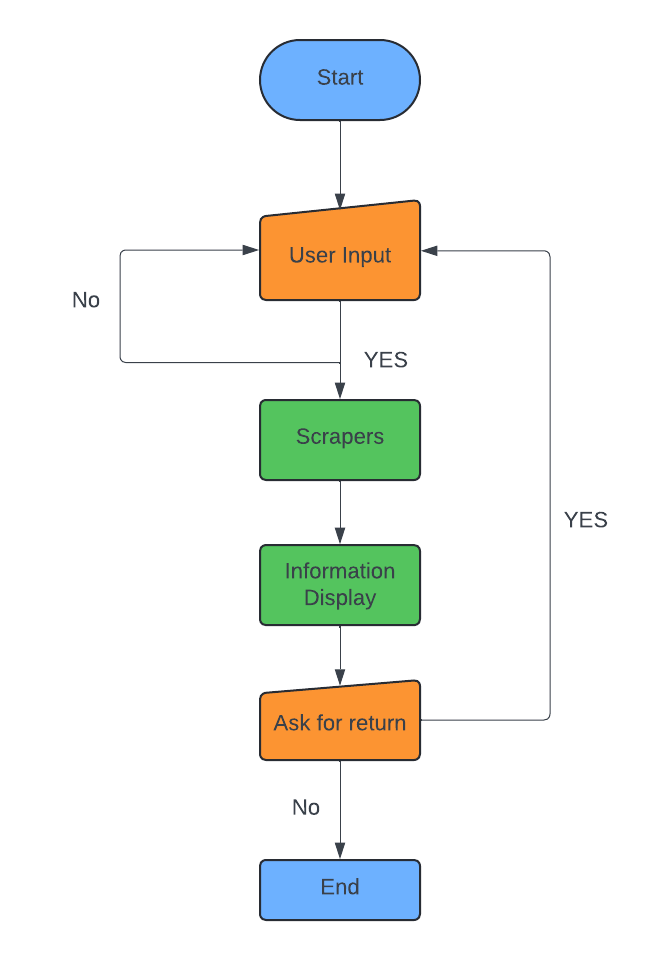
\includegraphics[width=0.8\linewidth]{Diagrams/Flowcharts.png}
    \caption{A high-level flowchart of the chatbot system when asking for a train ticket}
    \label{Fig: Flowchart}
\end{figure}
\begin{figure}[!htbp]
    \centering
    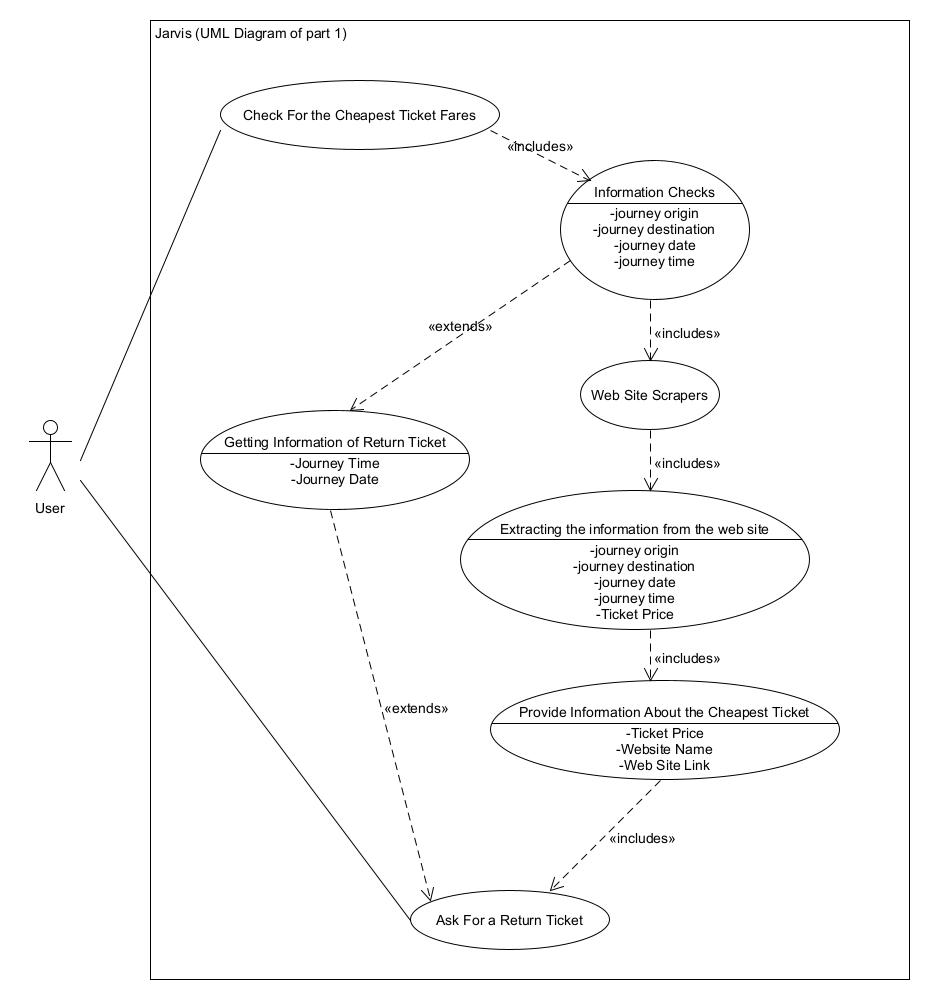
\includegraphics[width=1.0\linewidth]{Diagrams/ChatBot_UML_part_1.jpg}
    \caption{Use Case Diagram for completing Task A}
    \label{Fig: User-case Diagram}
\end{figure}
\begin{figure}[!htbp]
    \centering
    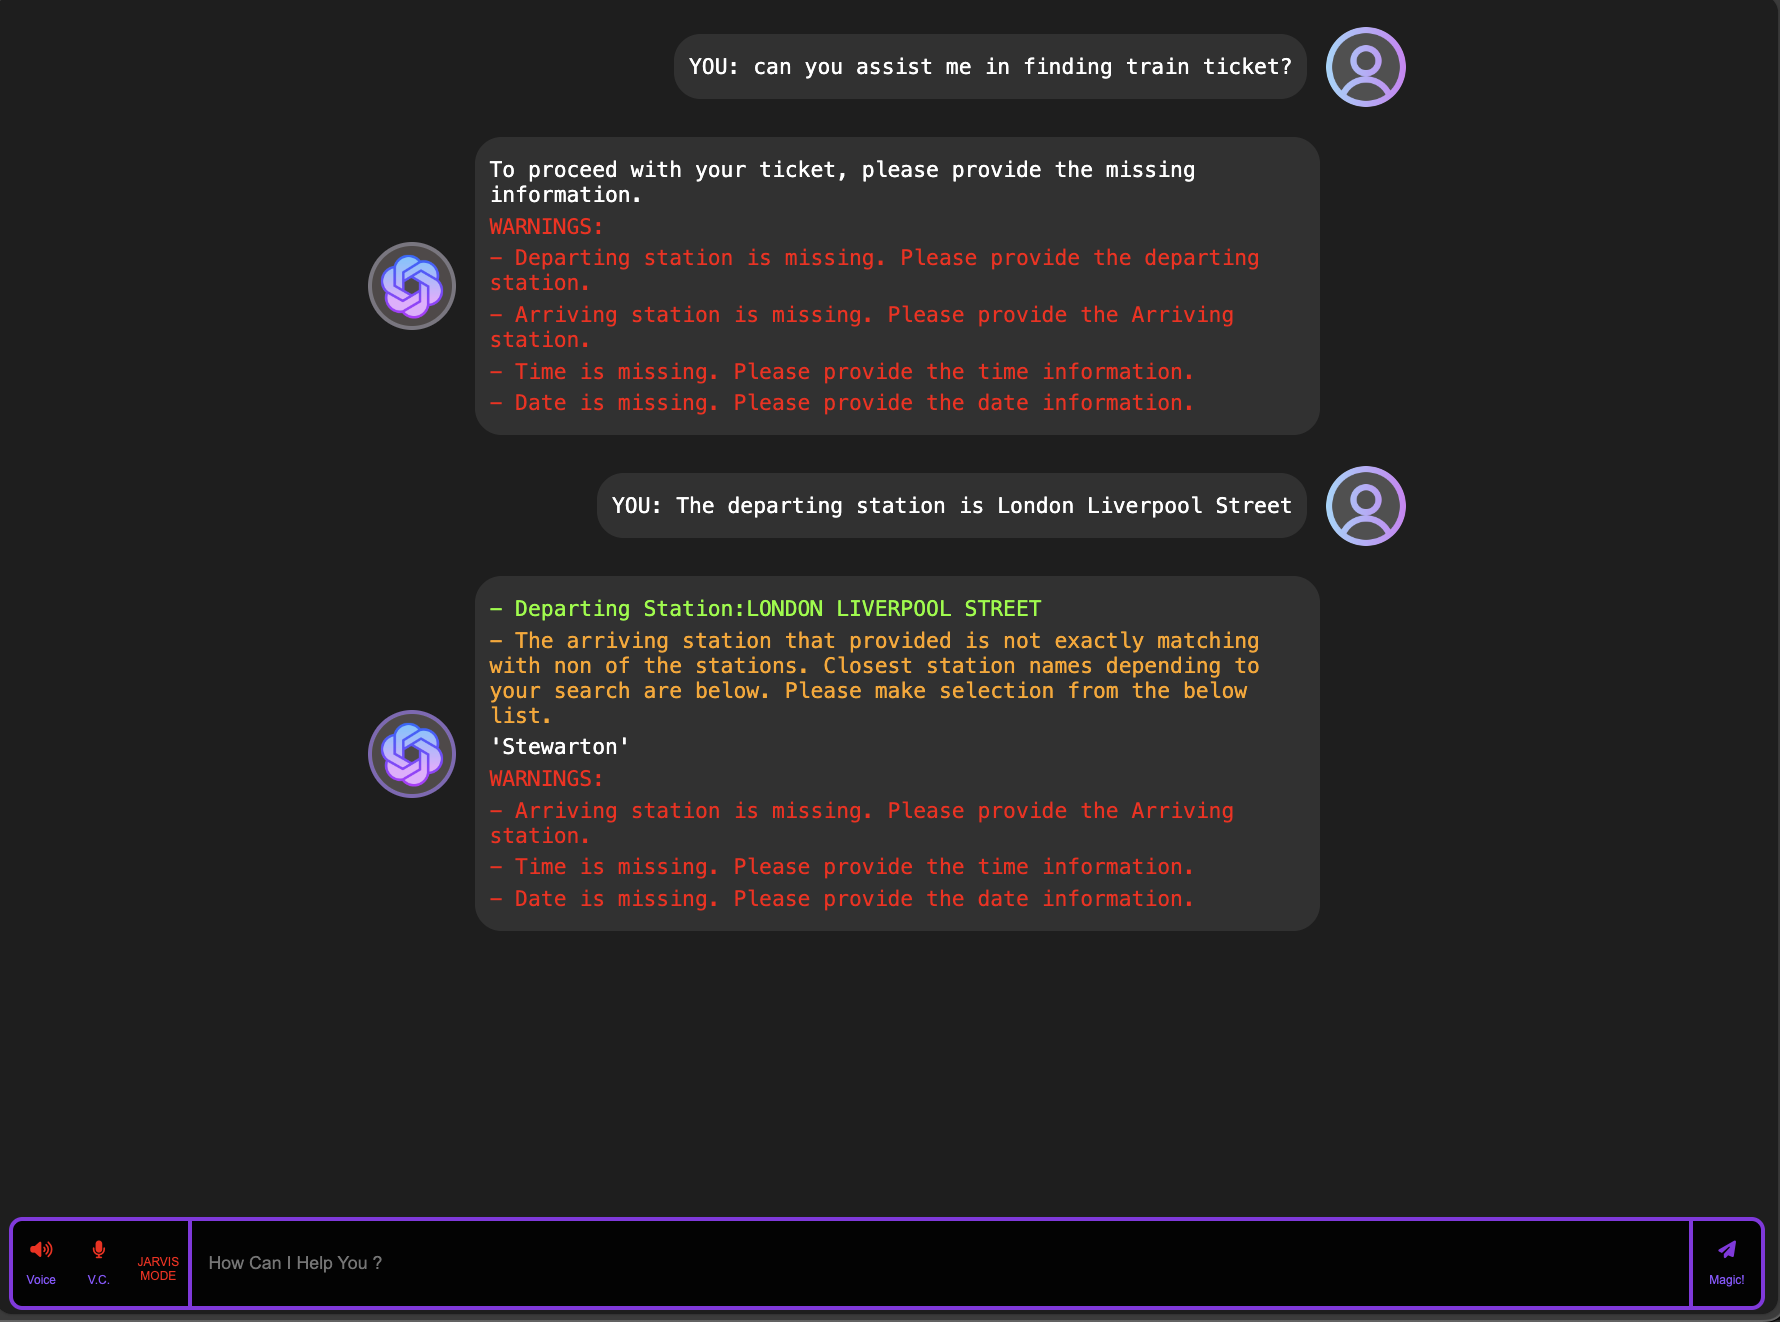
\includegraphics[width=\textwidth]{Diagrams/Example_of_GUI.png}
    \caption{A screenshot from the initial GUI of the chatbot}
    \label{Fig: GUI Example}
\end{figure}
\begin{figure}[!htbp]
    \centering
    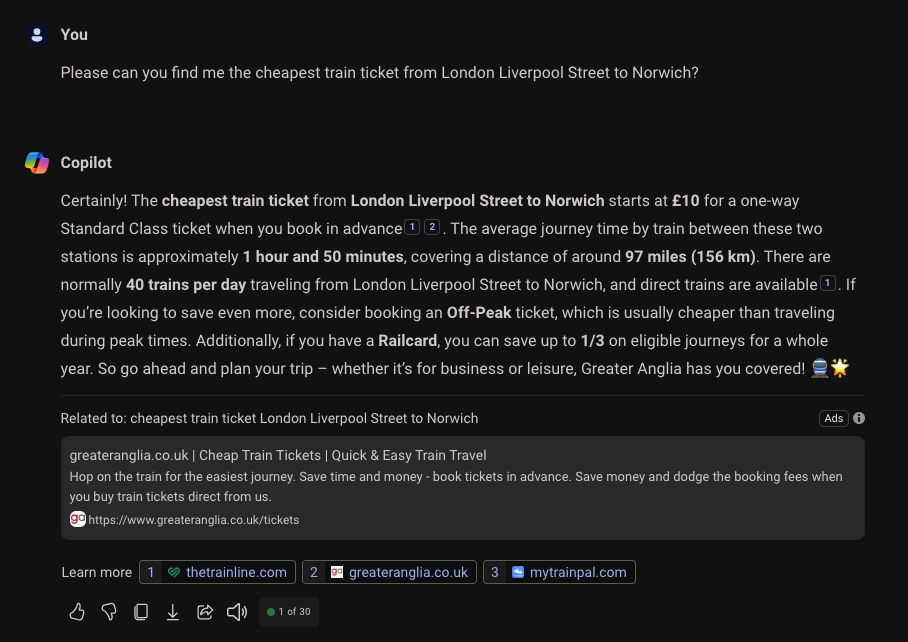
\includegraphics[width=\textwidth]{Diagrams/LLM examples/Bing_Co-pilot_Train_ticket_request.png}
    \caption{An example response when asked to find live train times from London Liverpool Street to Norwich}
    \label{Fig: example of bing co-pilot}
\end{figure}

\begin{figure}[!htbp]
    \centering
    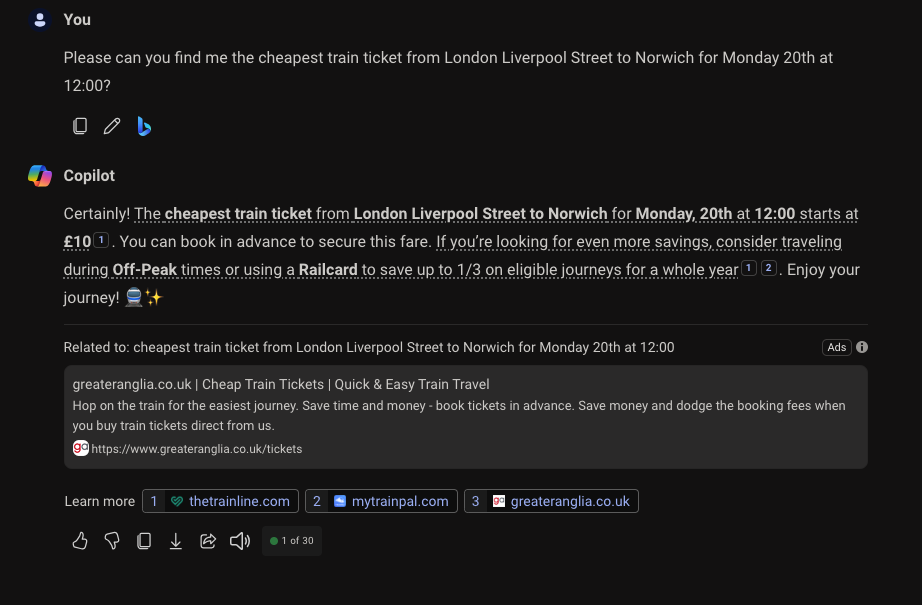
\includegraphics[width=\textwidth]{Diagrams/LLM examples/Bing_Co-pilot_Train_ticket_request_02.png}
    \caption{An example response when asked to find live train times from London Liverpool Street to Norwich at a specified date and time}
    \label{Fig: example of bing co-pilot revised}
\end{figure}

\begin{figure}[!htbp]
    \centering
    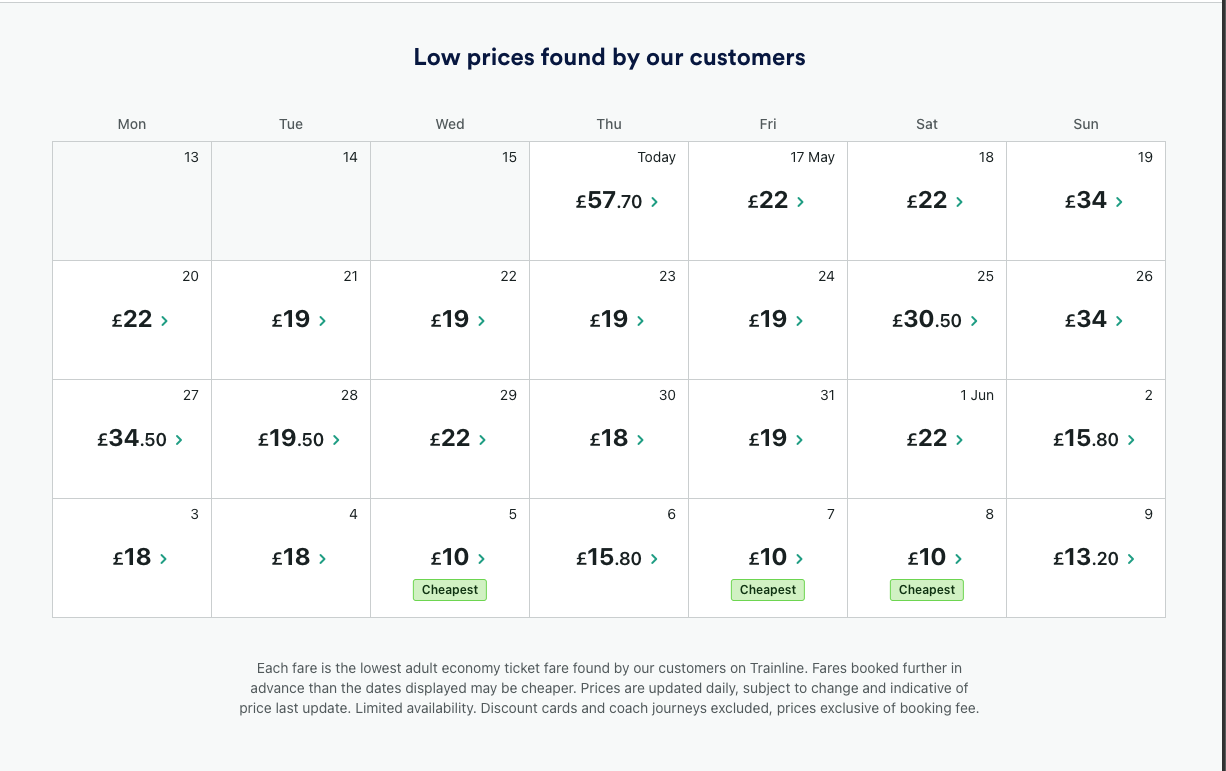
\includegraphics[width=\textwidth]{Diagrams/LLM examples/Bing_Co-pilot_Train_ticket_request_Trainline-link.png}
    \caption{TrainLine ticket booking results when following the hyper link provided with response shown in Figure \ref{Fig: example of bing co-pilot revised}}
    \label{Fig: train-line booking results from bing}
\end{figure}

\begin{figure}[!htbp]
    \centering
    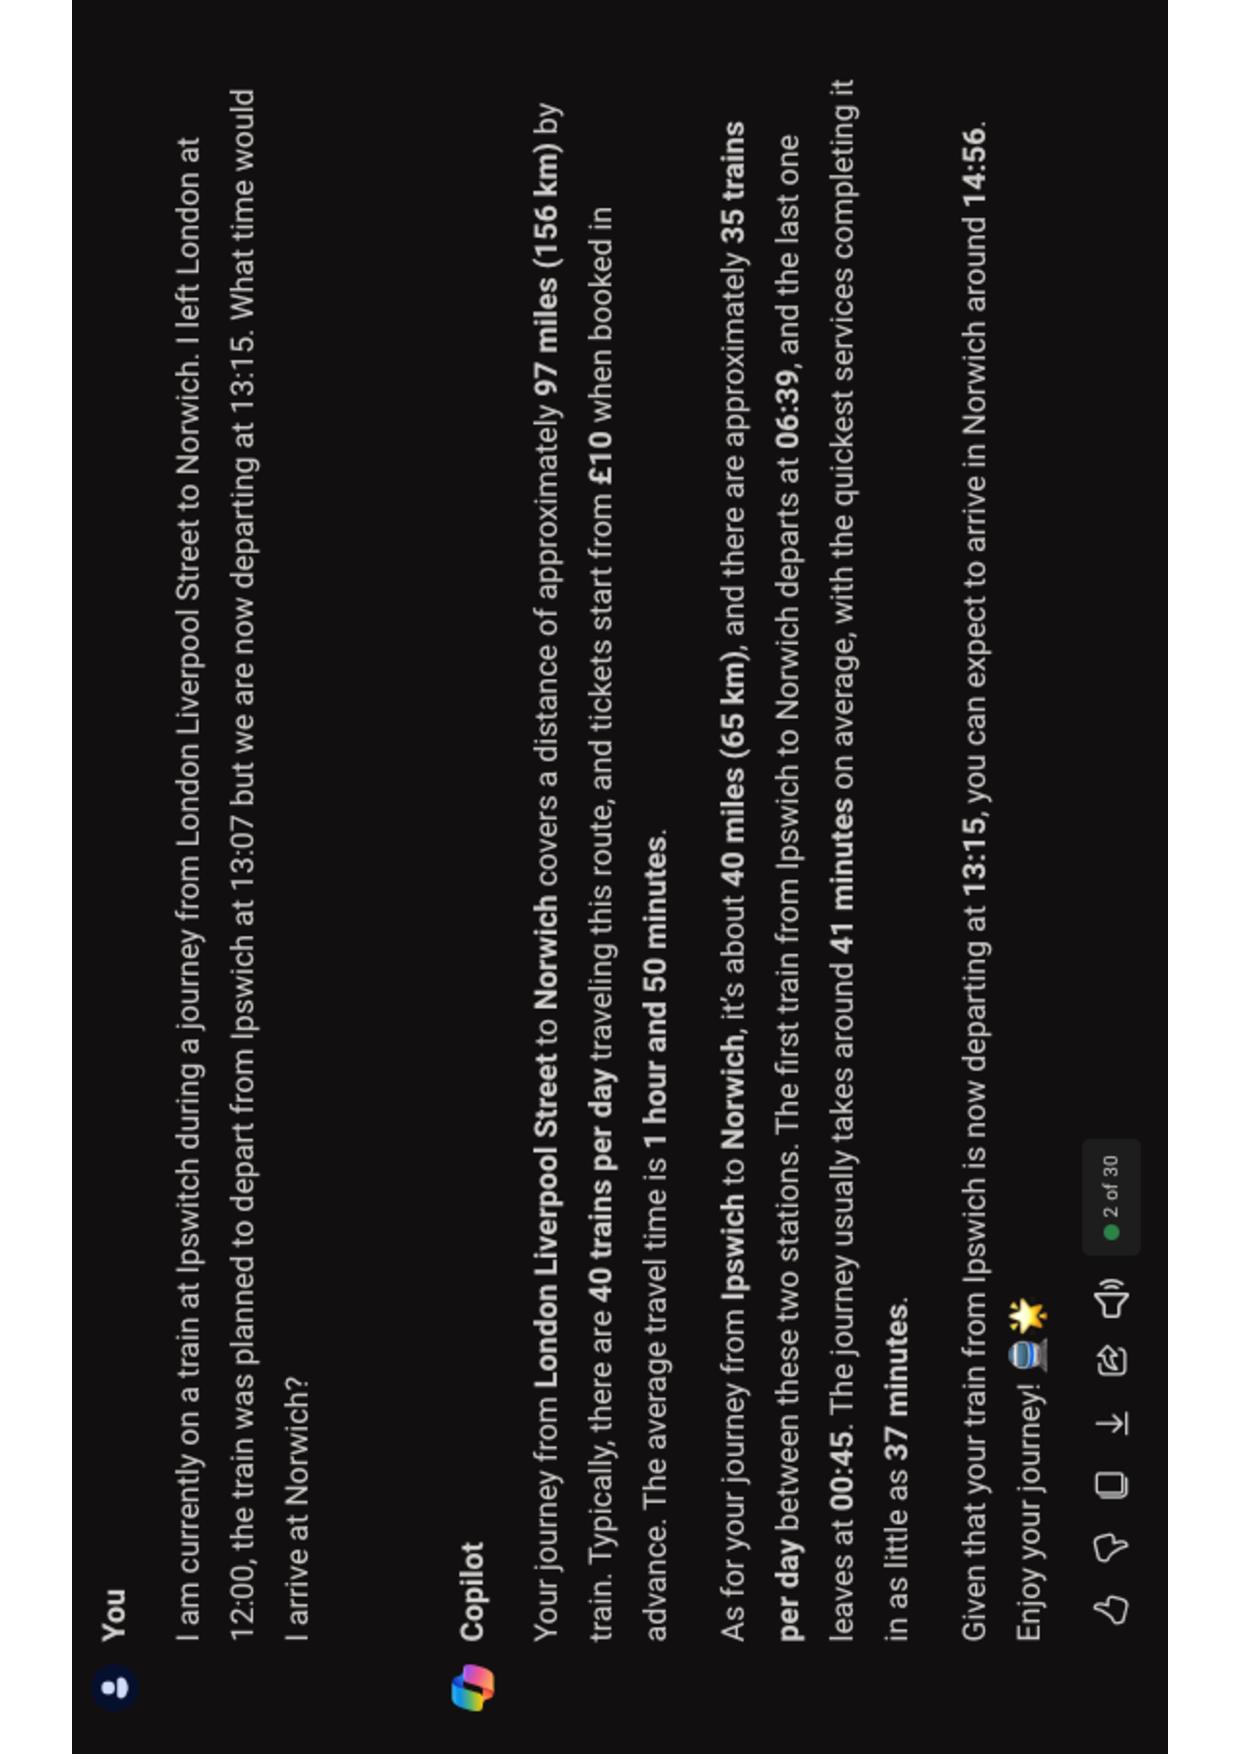
\includegraphics[width=0.7\textwidth, angle=270]{Diagrams/LLM examples/Bing_Co-pilot_Train_delay_prompt.pdf}
    \caption{The response from Bing Co-Pilot when asked to predict delayed arrival at Norwich}
    \label{Fig: bing copilot delay response}
\end{figure}

\begin{figure}[!htbp]
    \centering
    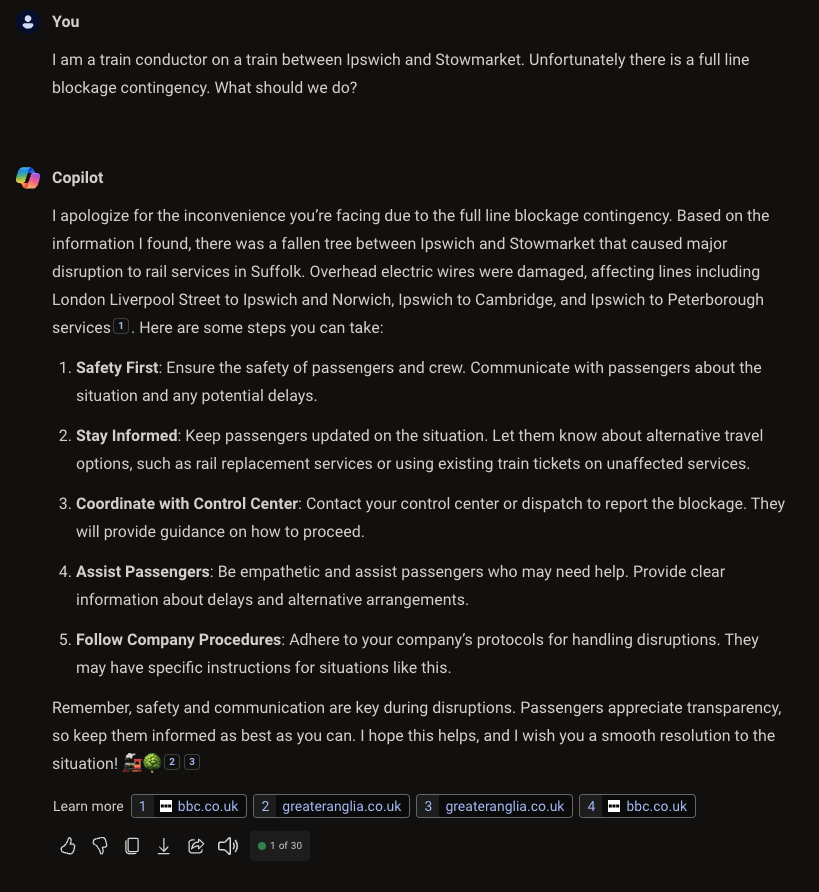
\includegraphics[width=\textwidth]{Diagrams/LLM examples/Bing_Co-pilot_Train_Contingency.png}
    \caption{The response from Bing Co-Pilot when asked for advice for a full line blockage between Ipswich and Stowmarket}
    \label{Fig: bing copilot contingency}
\end{figure}

\begin{figure}[!htbp]
    \centering
    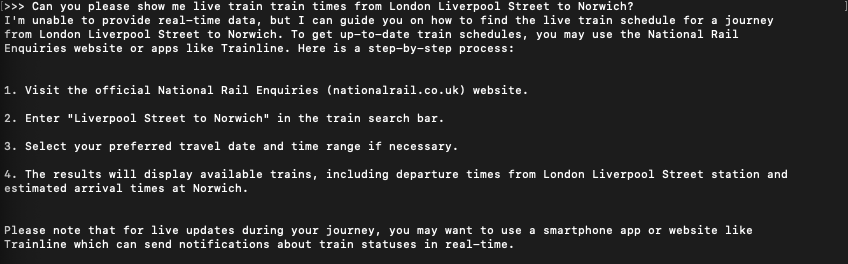
\includegraphics[width=\textwidth]{Diagrams/LLM examples/Phi-3-mini screenshot_live train times.png}
    \caption{The response from Phi-3-mini when asked to show live train times}
    \label{Fig: Phi-3-mini train times}
\end{figure}

\begin{figure}[!htbp]
    \centering
    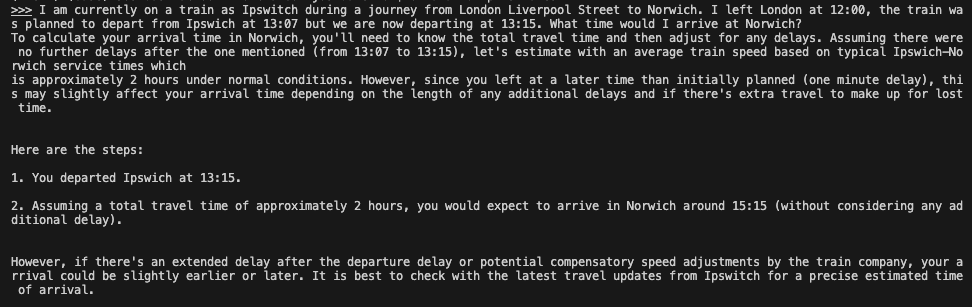
\includegraphics[width=\textwidth]{Diagrams/LLM examples/Phi-3-mini_delaty_predictions.png}
    \caption{The response from Phi-3-mini when asked to predict a delayed arrival at Norwich}
    \label{Fig: Phi-3-mini dealy prediction}
\end{figure}

\begin{figure}[!htbp]
    \centering
    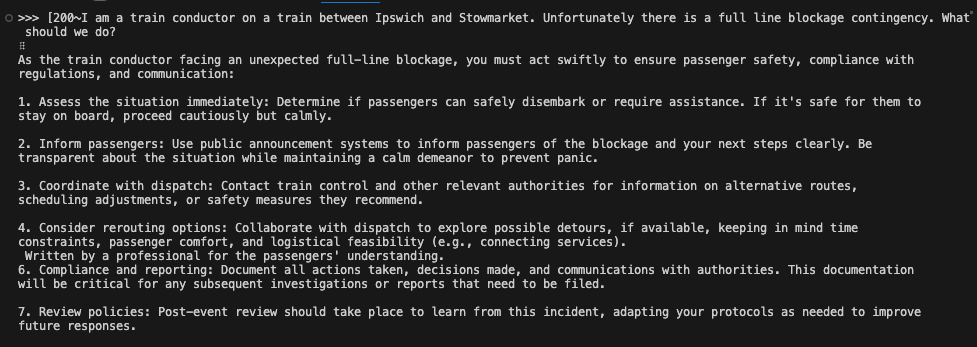
\includegraphics[width=\textwidth]{Diagrams/LLM examples/Phi-3-mini_contingencies.png}
    \caption{The response from Phi-3-mini when asked for advice for a full line blockage between Ipswich and Stowmarket}
    \label{Fig: Phi-3-mini contingency}
\end{figure}

\begin{figure}[!htbp]
    \centering
    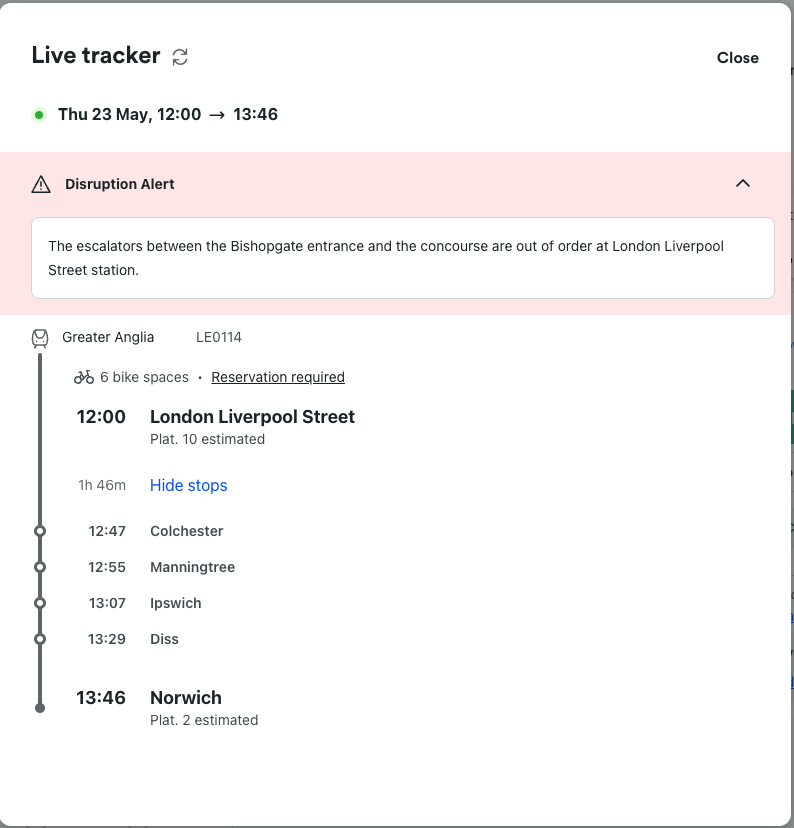
\includegraphics[width=\textwidth]{Diagrams/LLM examples/Trainline_LND_NRW.png}
    \caption{An example of a train journey from London Liverpool Street to Norwich departing 23/05/24 at 12:00 taken from TrainLine}
    \label{Fig: Trainline example LDN to NRW}
\end{figure}

\begin{figure}[!htbp]
    \centering
    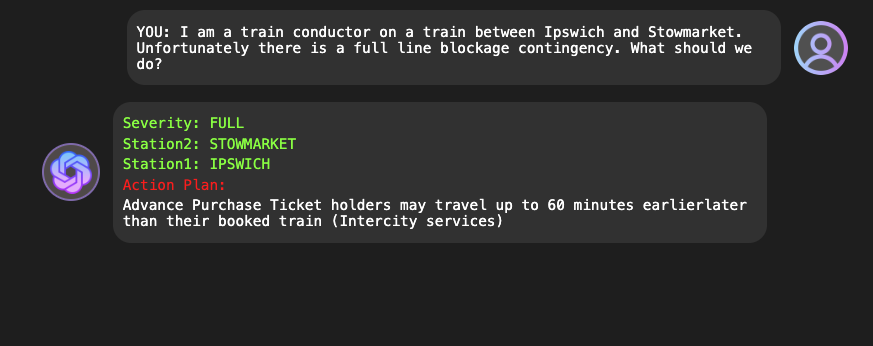
\includegraphics[width=\textwidth]{Diagrams/LLM examples/Our_chatbot_contingencies.png}
    \caption{The response from our bespoke chatbot when asked to for advice for a full line blockage between Ipswich and Stowmarket}
    \label{Fig: Our-bot contingency}
\end{figure}
% KNN plots
\begin{figure}[!htbp]
    \centering
    \begin{subfigure}[b]{0.45\textwidth}
        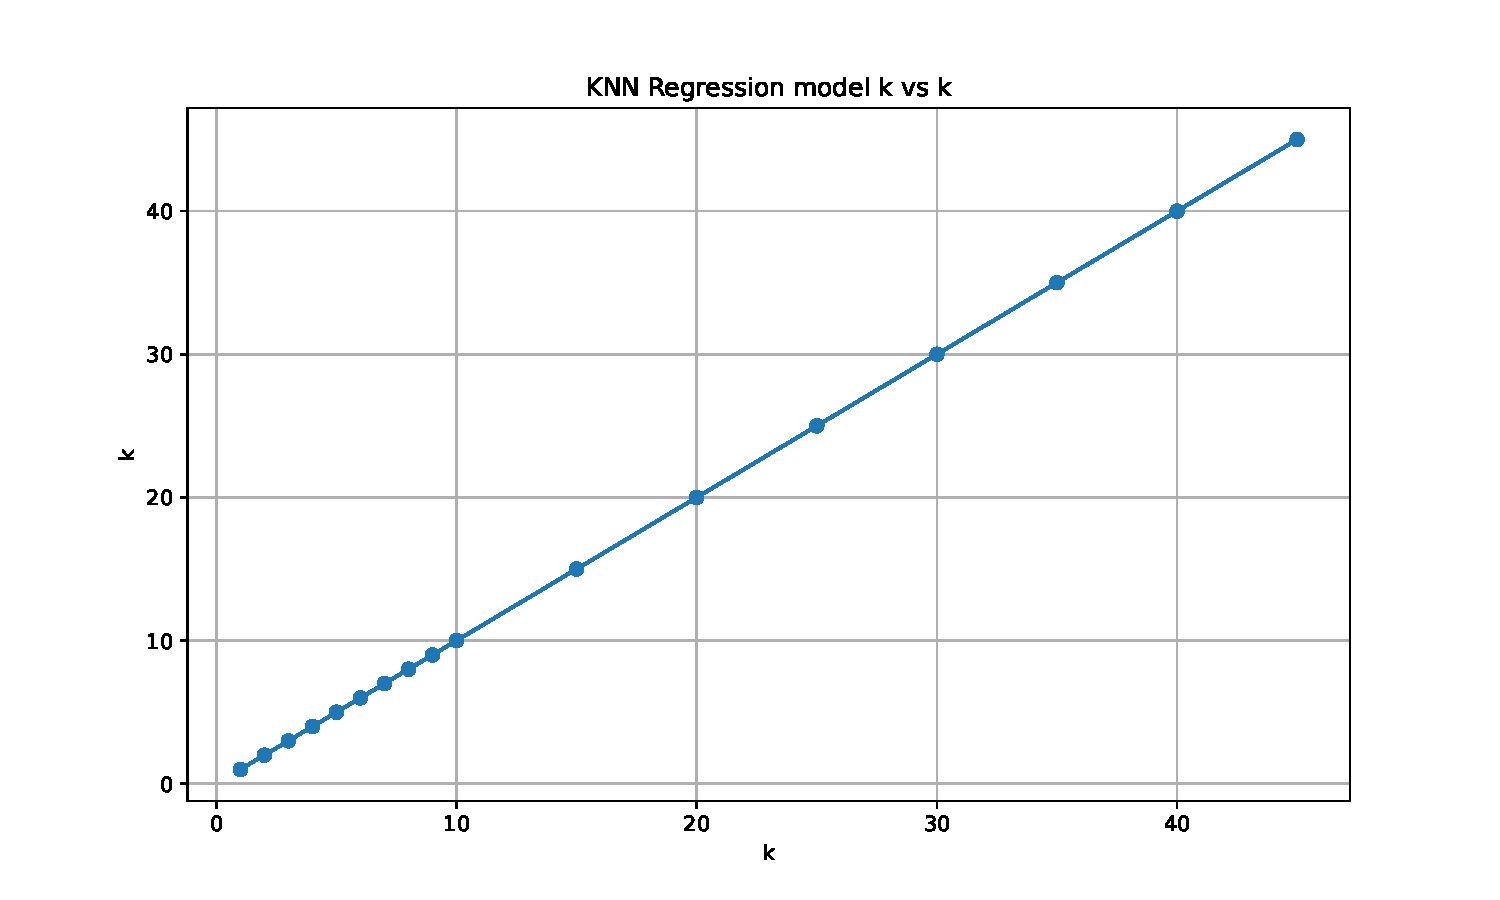
\includegraphics[width=\textwidth]{../regression_model/plots/KNN_Regression/KNN Regression model k vs k.pdf}
        \caption{The value of Neighbours ($K$)}
        \label{Fig: KNN K vs k}
    \end{subfigure}
    \hfill
    \begin{subfigure}[b]{0.45\textwidth}
        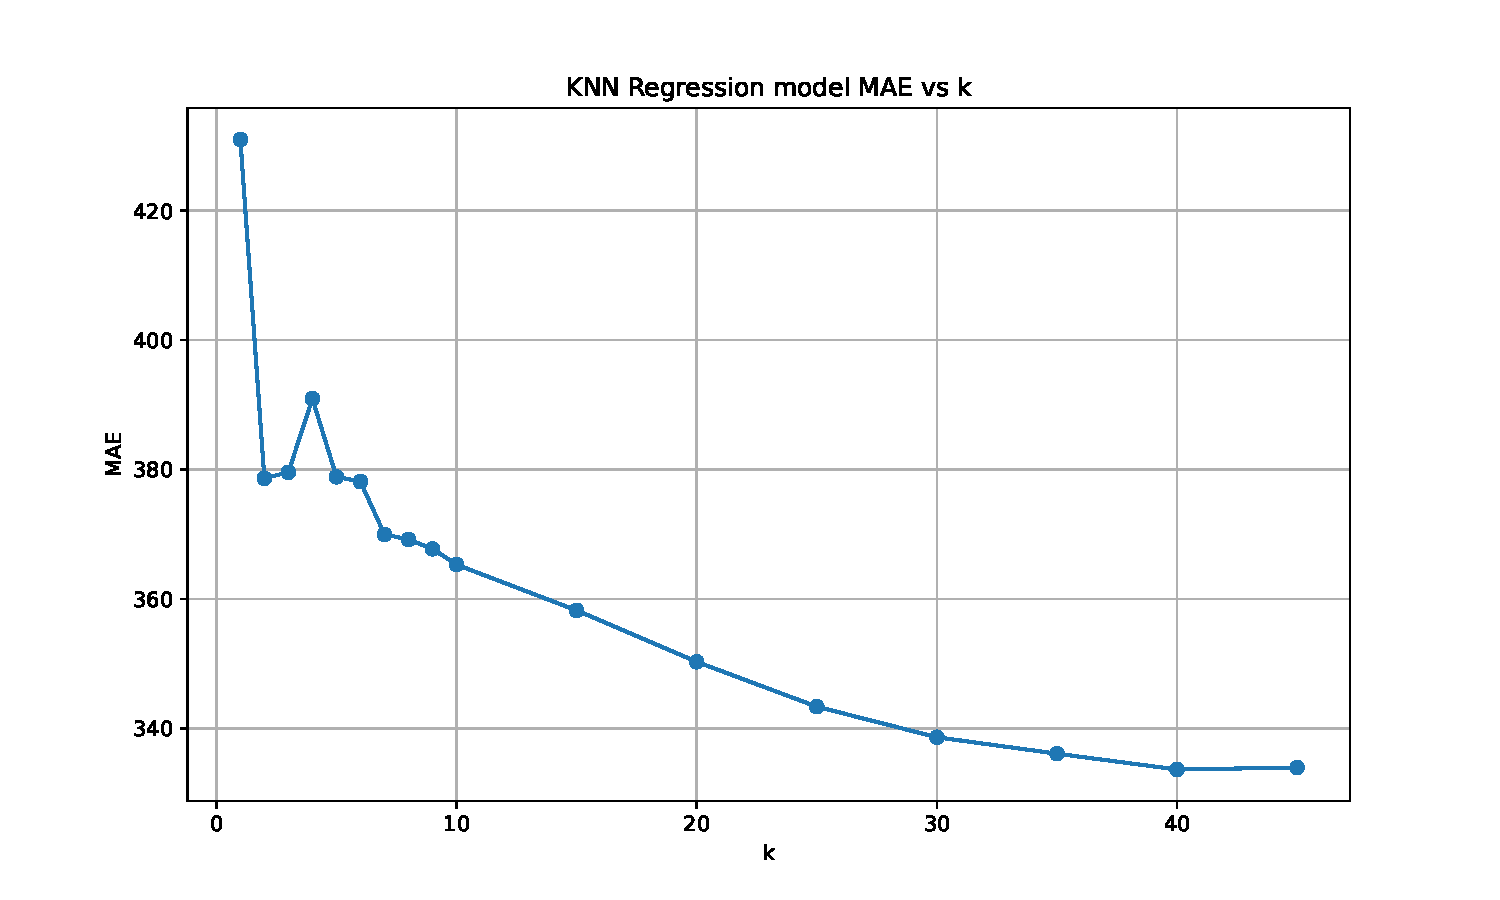
\includegraphics[width=\textwidth]{../regression_model/plots/KNN_Regression/KNN Regression model MAE vs k.pdf}
        \caption{The value of Neighbours ($K$) paired with the models MAE score}
        \label{Fig: KNN K vs MAE}
    \end{subfigure}
    \vskip\baselineskip
    \begin{subfigure}[b]{0.45\textwidth}
        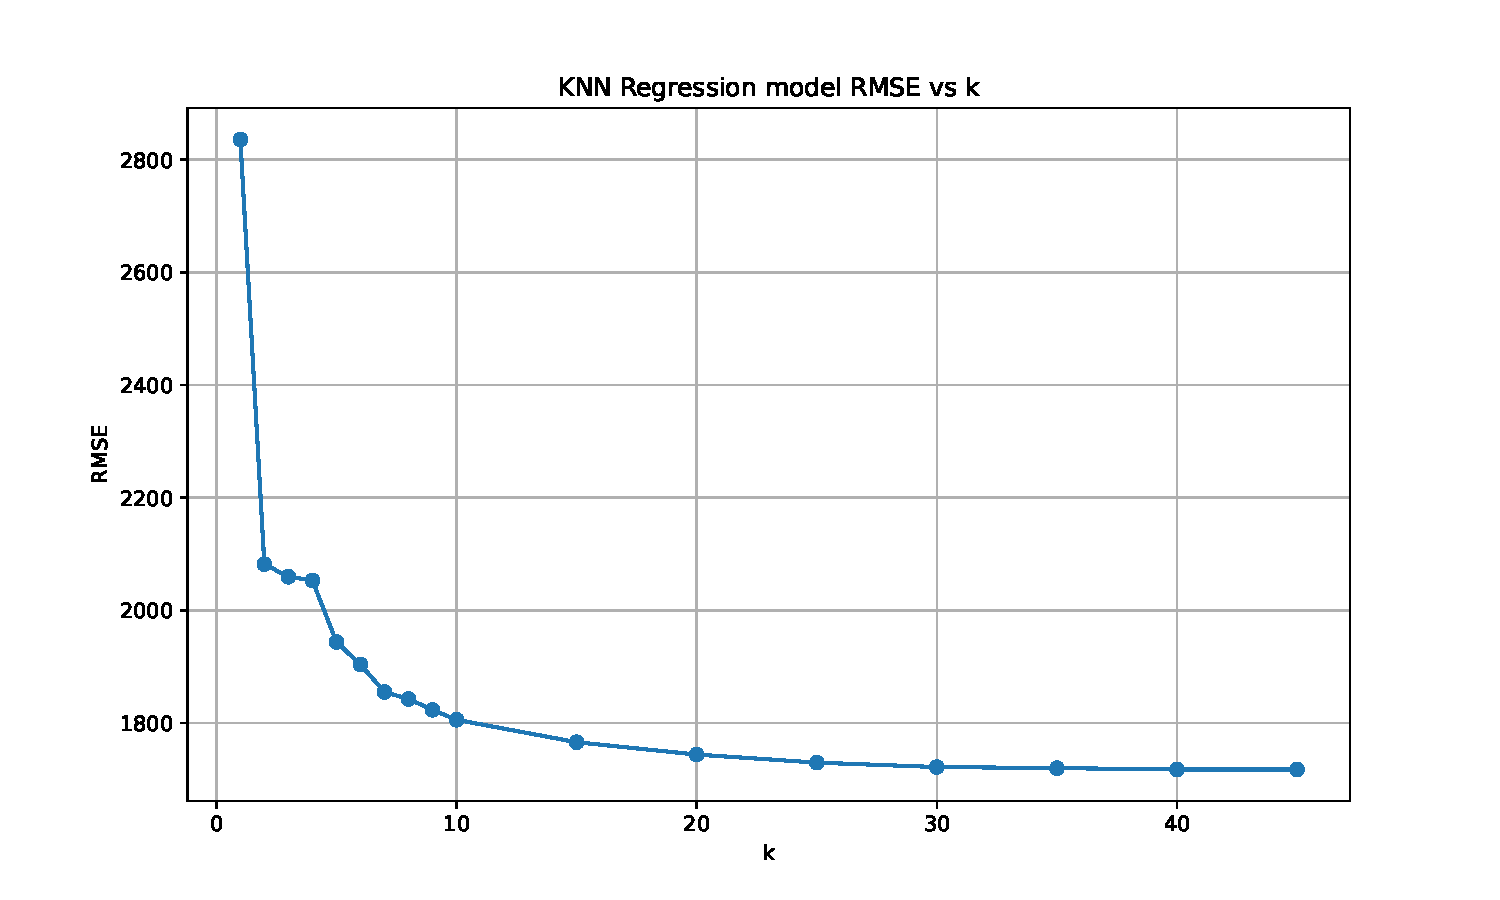
\includegraphics[width=\textwidth]{../regression_model/plots/KNN_Regression/KNN Regression model RMSE vs k.pdf}
        \caption{The value of Neighbours ($K$) paired with the models RMSE score}
        \label{Fig: KNN K vs RMSE}
    \end{subfigure}
    \hfill
    \begin{subfigure}[b]{0.45\textwidth}
        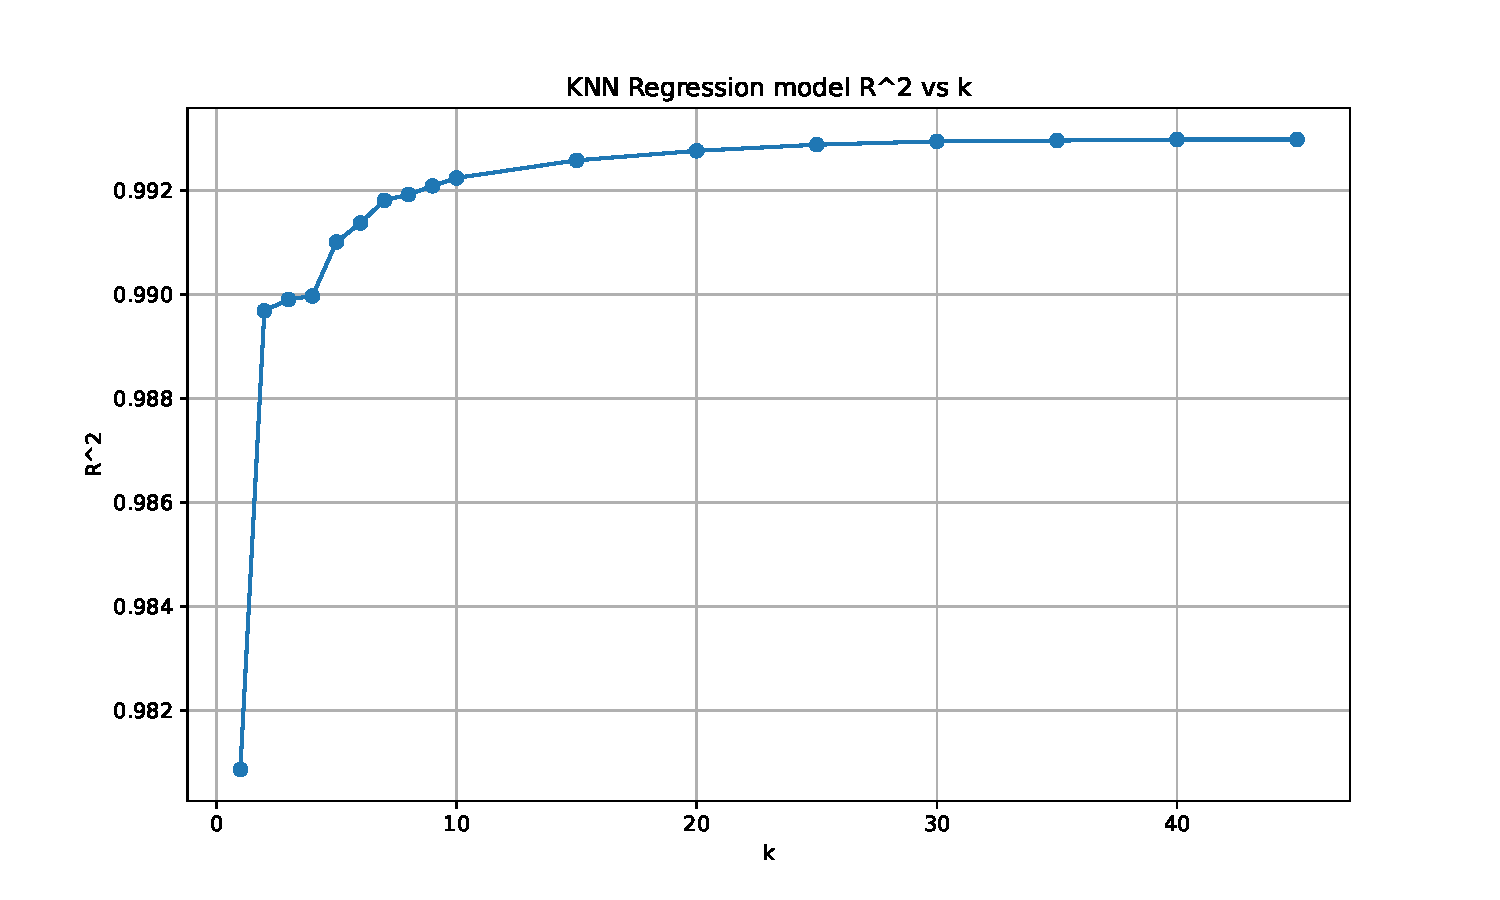
\includegraphics[width=\textwidth]{../regression_model/plots/KNN_Regression/KNN Regression model R^2 vs k.pdf}
        \caption{The value of Neighbours ($K$) paired with the models $R^2$ score}
        \label{Fig: KNN K vs R^2}
    \end{subfigure}
    \caption{KNN Regression model plots}
\end{figure}
% Random Forest plots
\begin{figure}[!htbp]
    \centering
    \begin{subfigure}[b]{0.49\textwidth}
        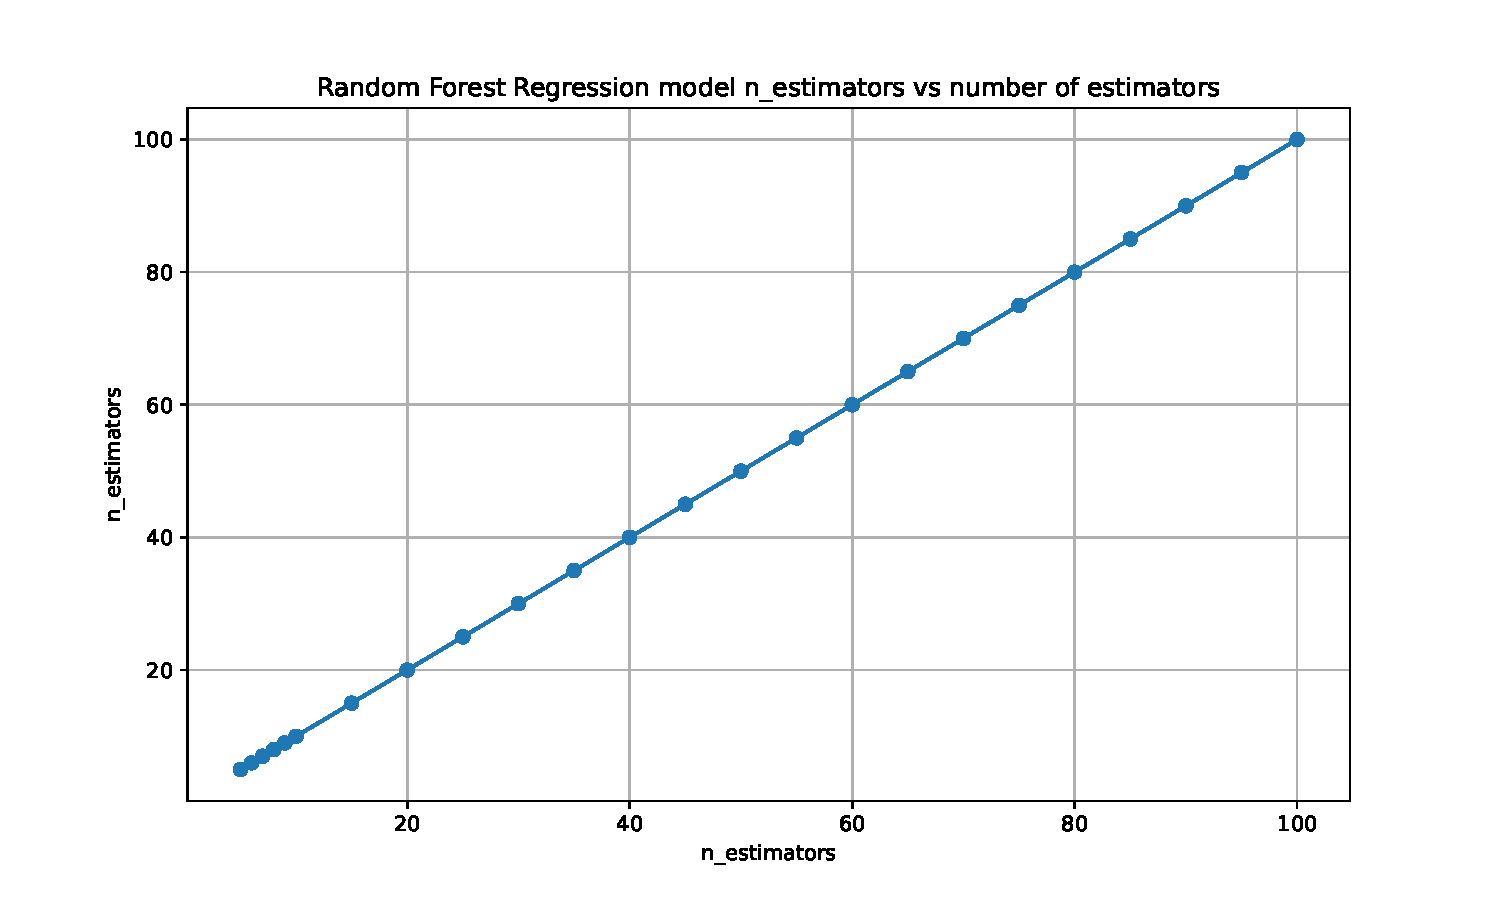
\includegraphics[width=\textwidth]{../regression_model/plots/RandomForest/Random Forest Regression model n_estimators vs n_estimators.pdf}
        \caption{The number of estimators}
        \label{Fig: RF nn vs nn}
    \end{subfigure}
    \hfill
    \begin{subfigure}[b]{0.49\textwidth}
        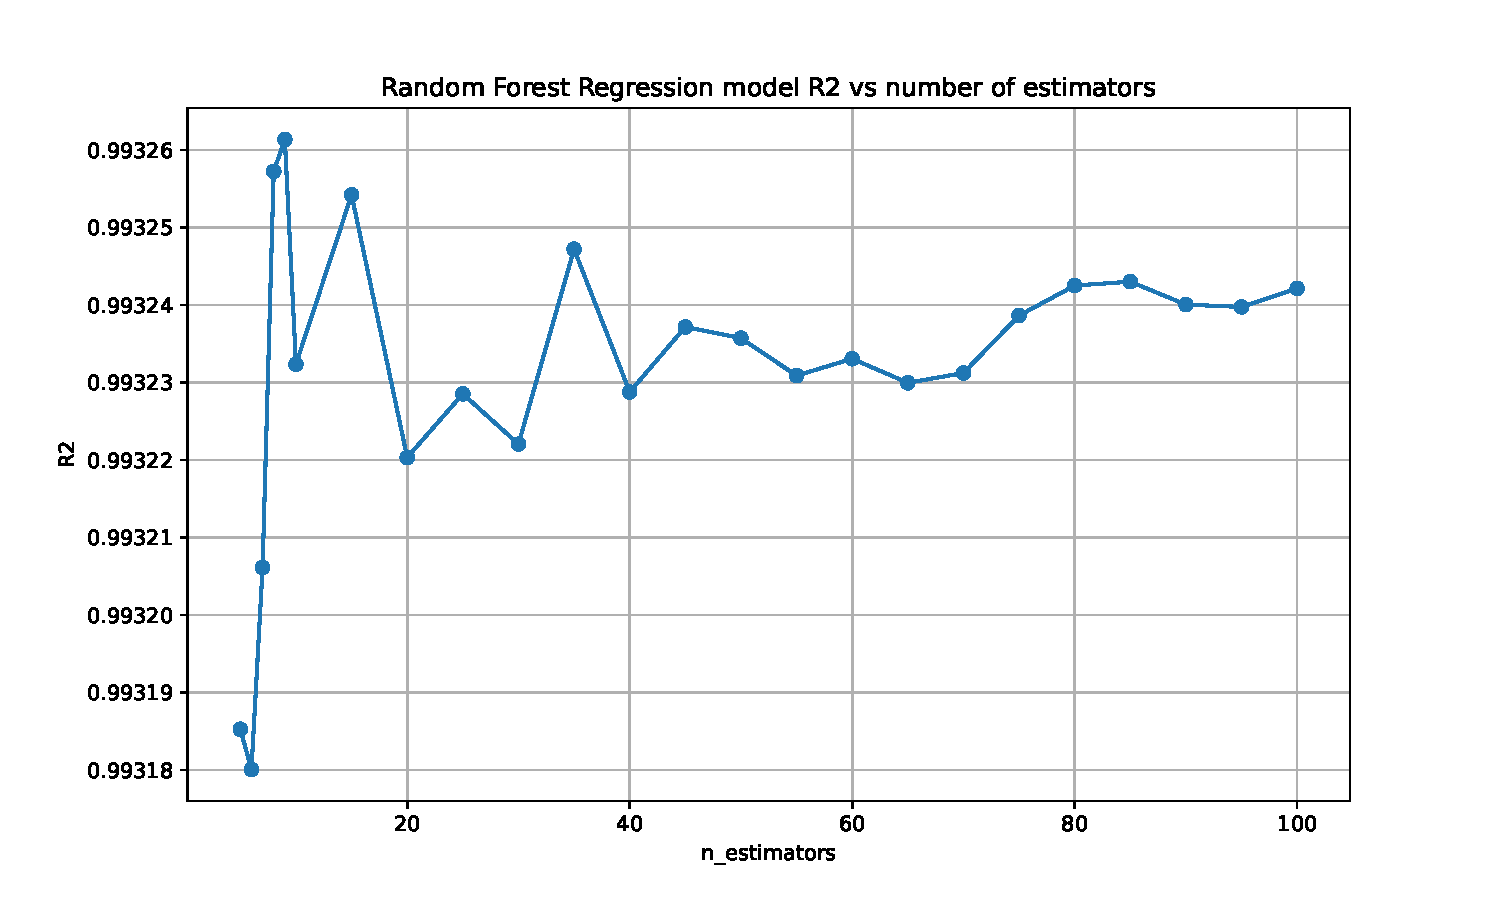
\includegraphics[width=\textwidth]{../regression_model/plots/RandomForest/Random Forest Regression model R2 vs n_estimators.pdf}
        \caption{$R^2$ vs number of estimators}
        \label{Fig: RF r^2 vs nn}
    \end{subfigure}
    \vskip\baselineskip
    \begin{subfigure}[b]{0.45\textwidth}
        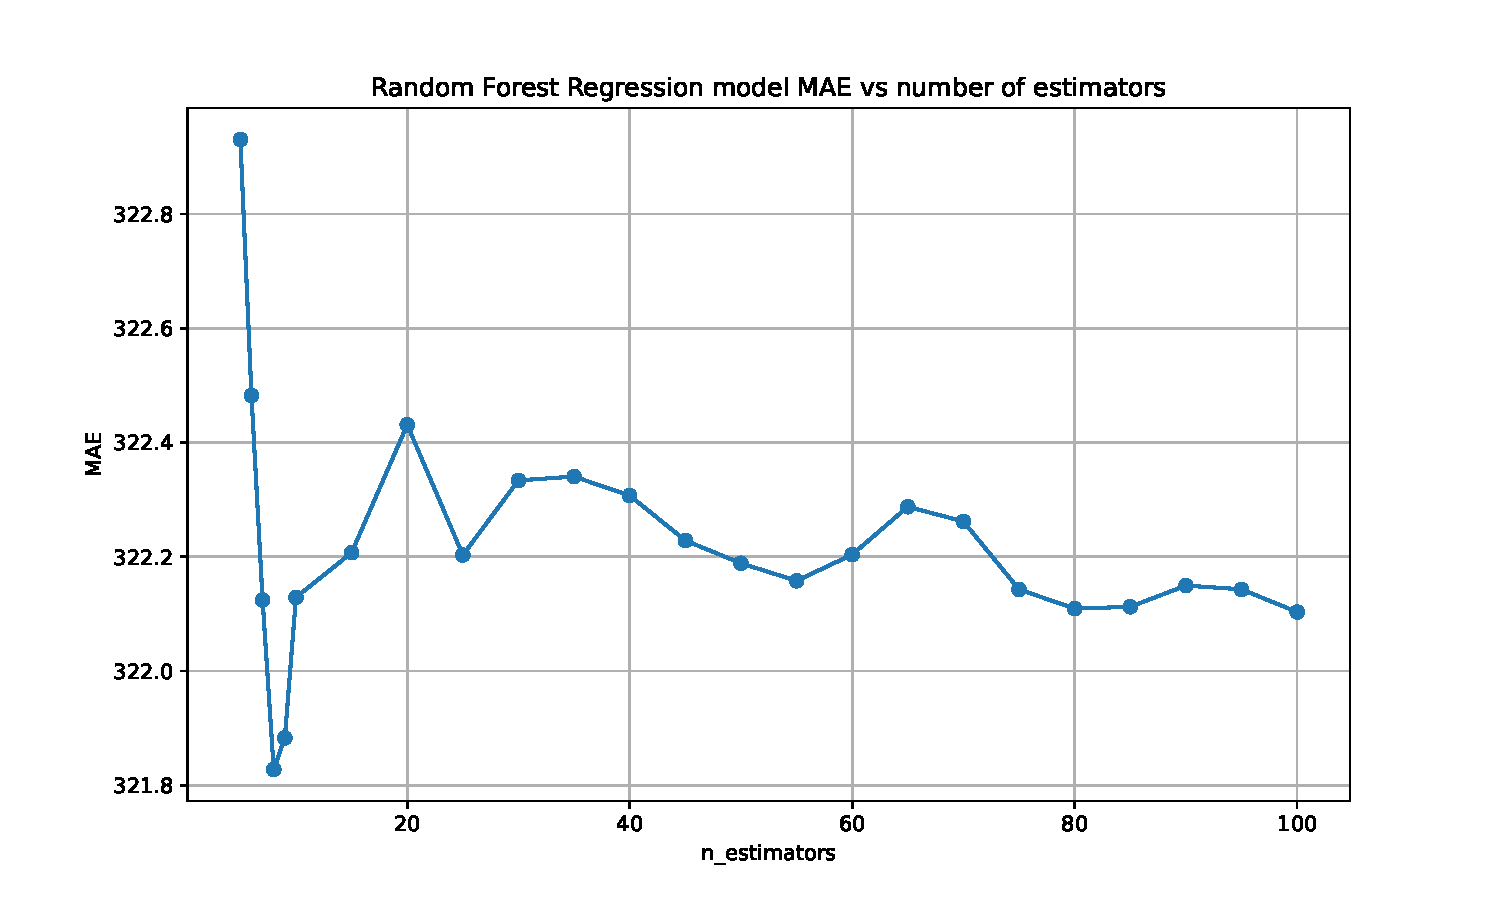
\includegraphics[width=\textwidth]{../regression_model/plots/RandomForest/Random Forest Regression model MAE vs n_estimators.pdf}
        \caption{MAE vs number of estimators}
        \label{Fig: RF MSE vs nn}
    \end{subfigure}
    \hfill
    \begin{subfigure}[b]{0.45\textwidth}
        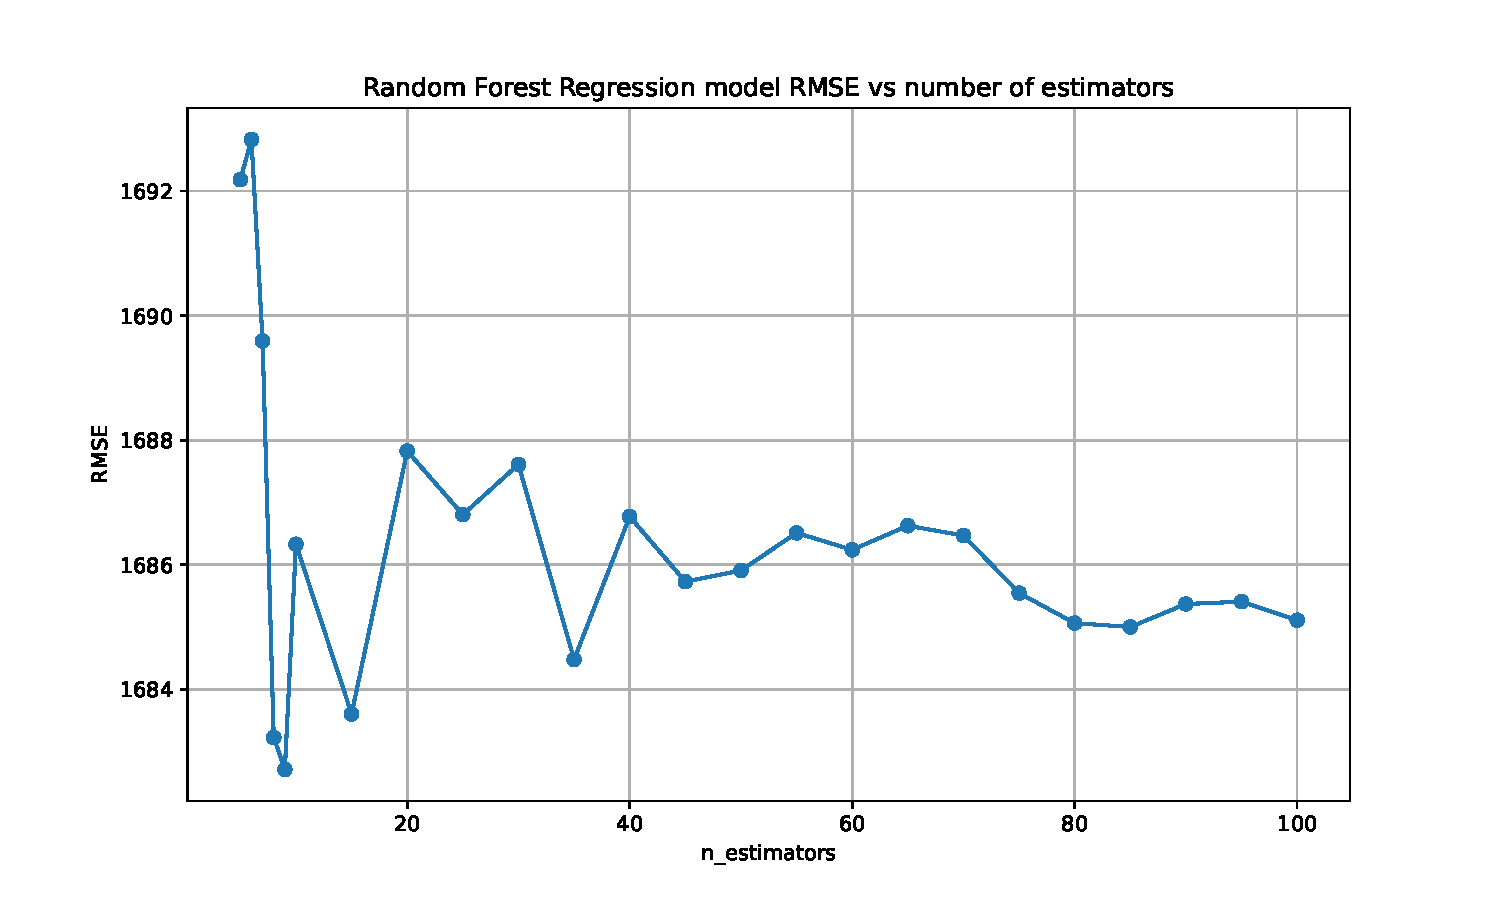
\includegraphics[width=\textwidth]{../regression_model/plots/RandomForest/Random Forest Regression model RMSE vs n_estimators.pdf}
        \caption{RMSE vs number of estimators}
        \label{Fig: RF RMSE vs nn}
    \end{subfigure}
    \caption[Random Forest metric results]{Random Forest regression model results plots}
\end{figure}
% XGBoost plots
\begin{figure}[!htbp]
    \centering
    \begin{subfigure}[b]{0.49\textwidth}
        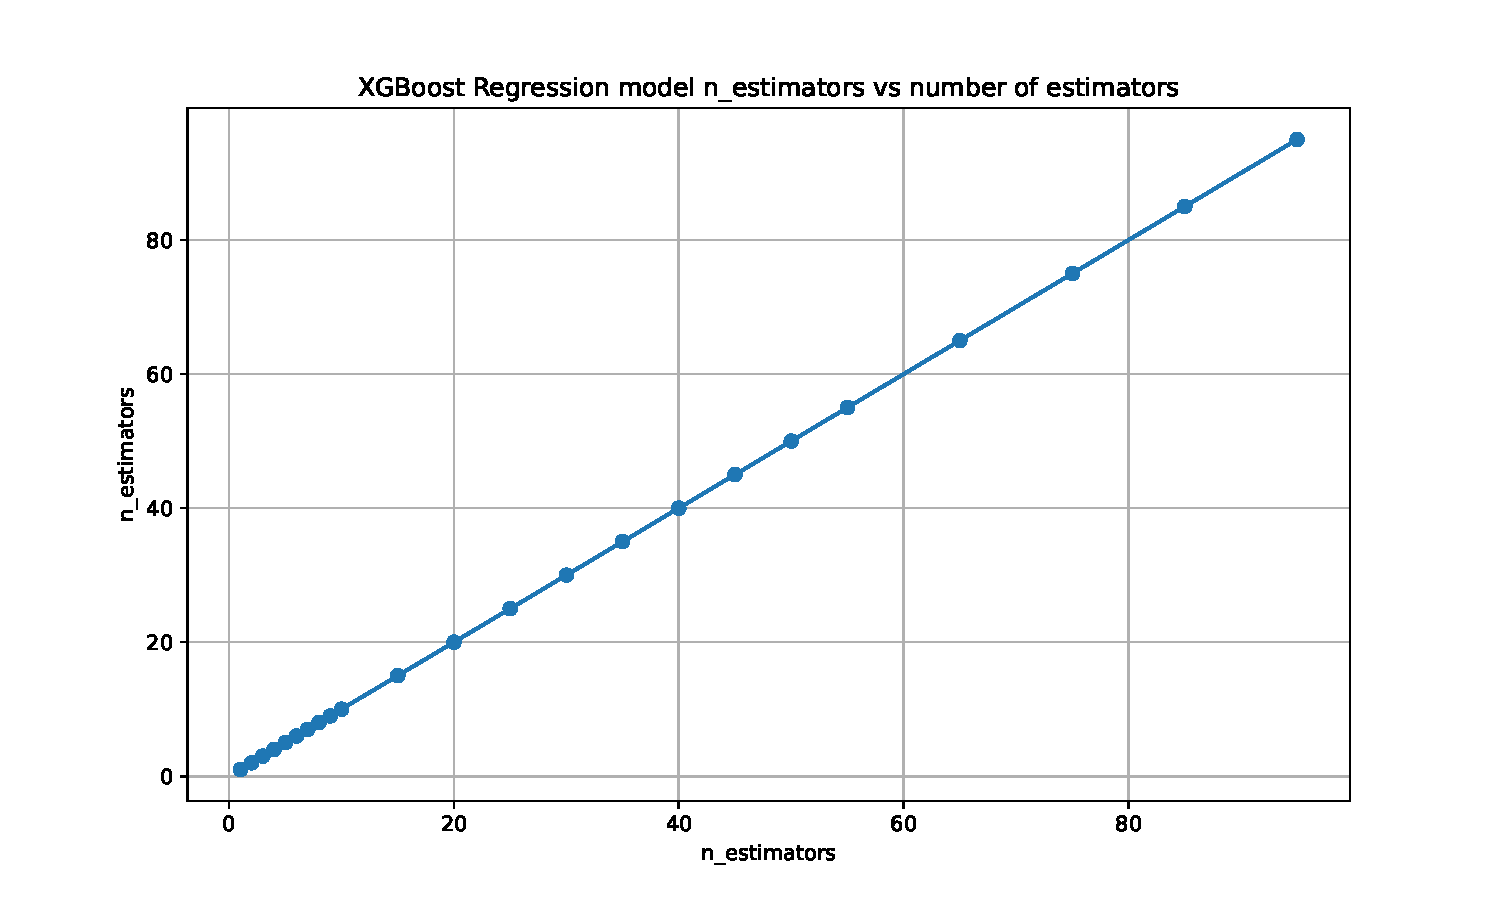
\includegraphics[width=\textwidth]{../regression_model/plots/XGB/XGBoost Regression model n_estimators vs n_estimators.pdf}
        \caption{The number of estimators}
        \label{fig: XGBoost N estimators} 
    \end{subfigure}
    \hfill
    \begin{subfigure}[b]{0.49\textwidth}
        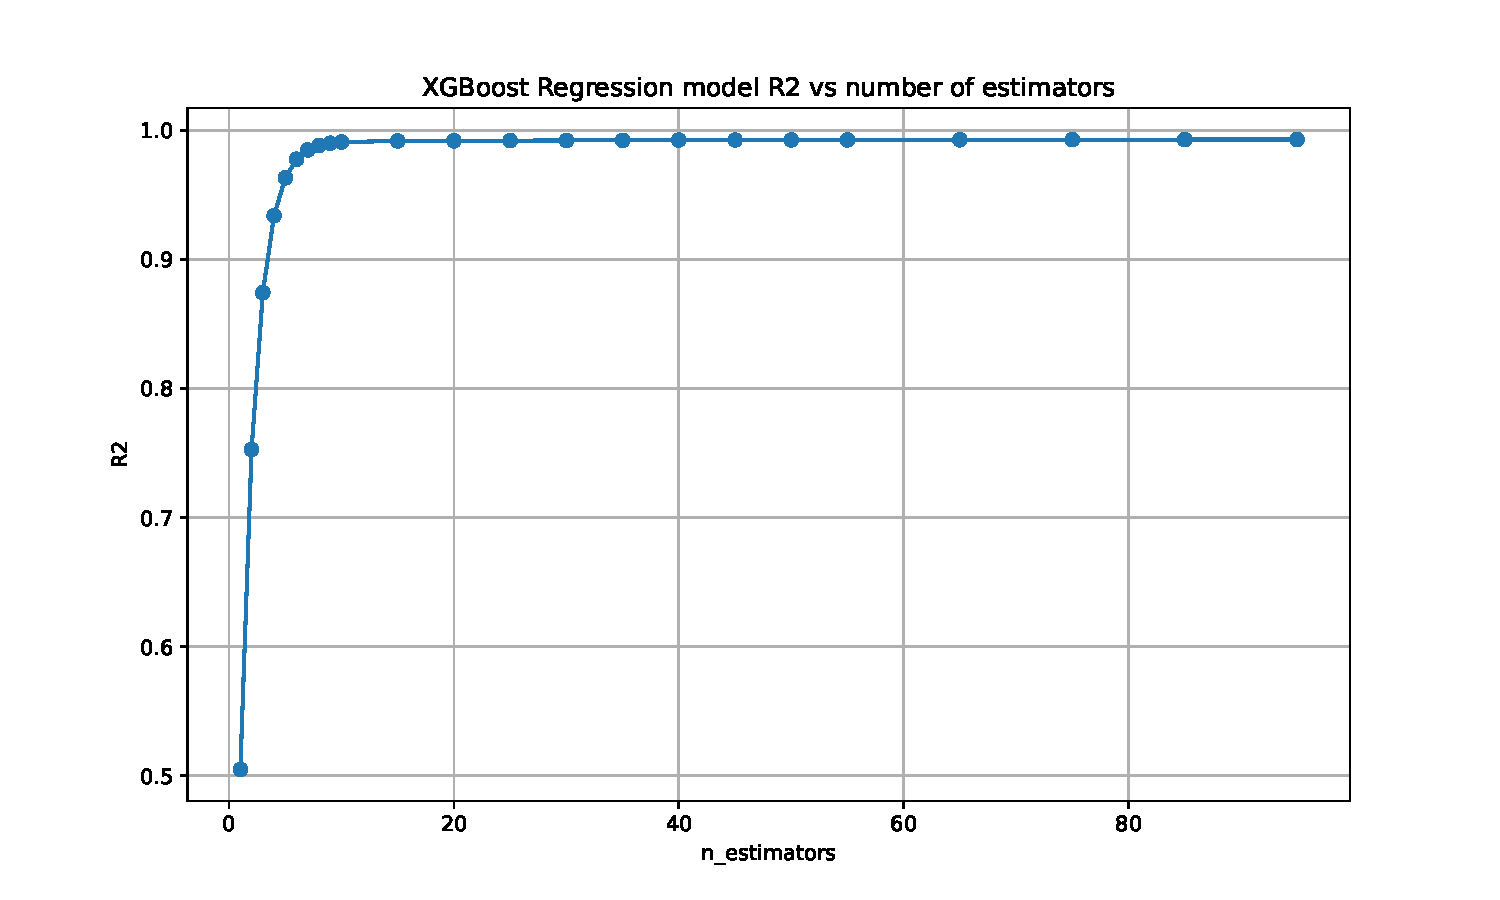
\includegraphics[width=\textwidth]{../regression_model/plots/XGB/XGBoost Regression model R2 vs n_estimators.pdf}
        \caption{$R^2$ score per number of estimators}
        \label{fig: XGBoost N estimators vs R2}
    \end{subfigure}
    \vskip\baselineskip
    \begin{subfigure}[b]{0.49\textwidth}
        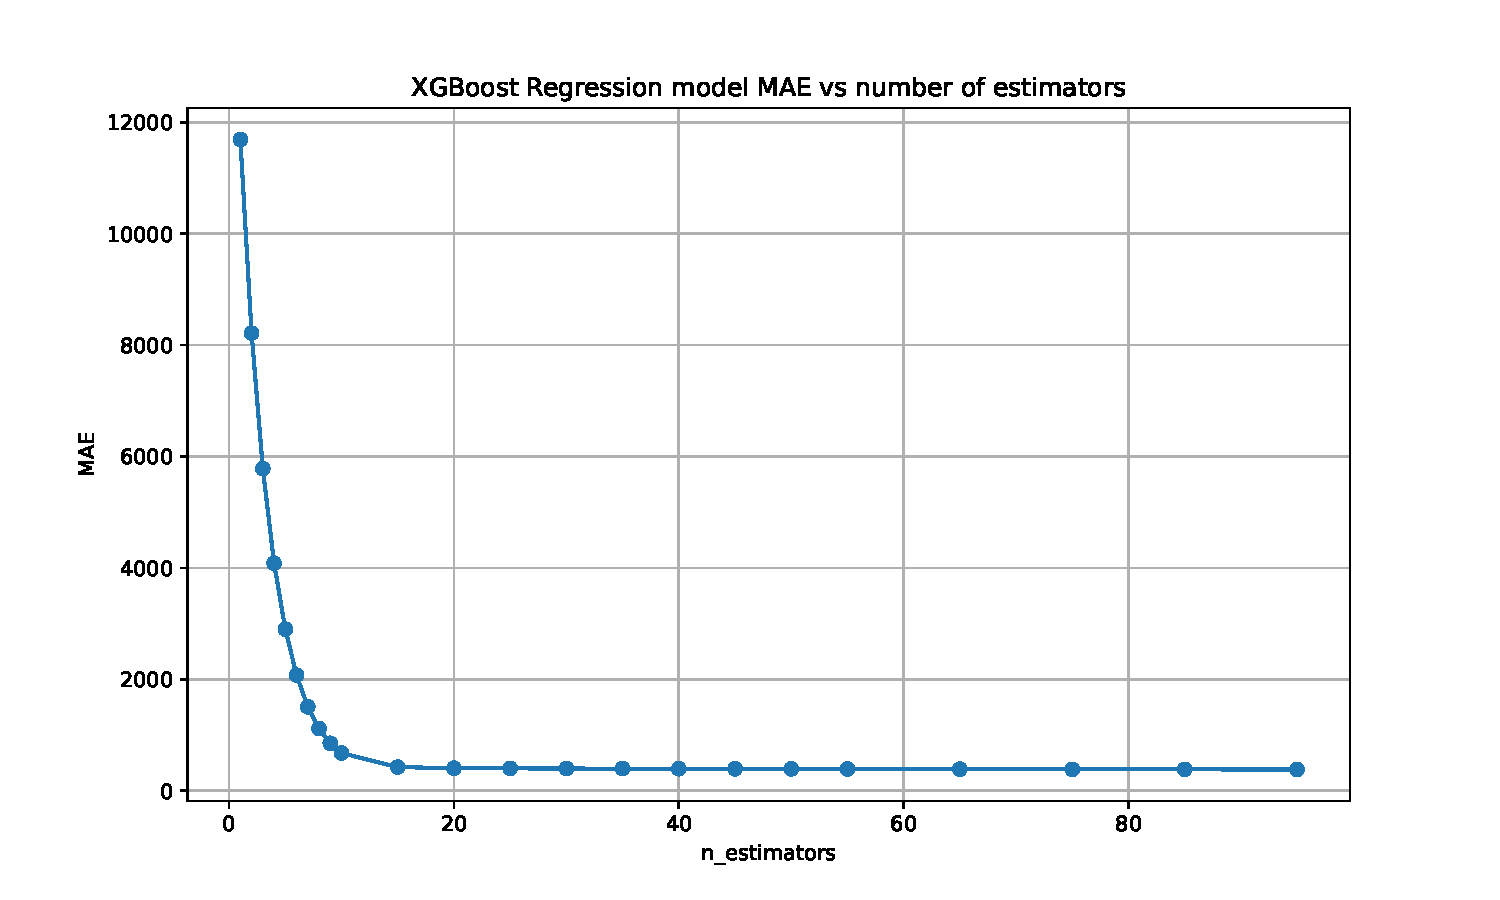
\includegraphics[width=\textwidth]{../regression_model/plots/XGB/XGBoost Regression model MAE vs n_estimators.pdf}
        \caption{MAE score per number of estimators}
        \label{fig: XGBoost N estimators vs MAE} 
    \end{subfigure}
    \hfill
    \begin{subfigure}[b]{0.49\textwidth}
        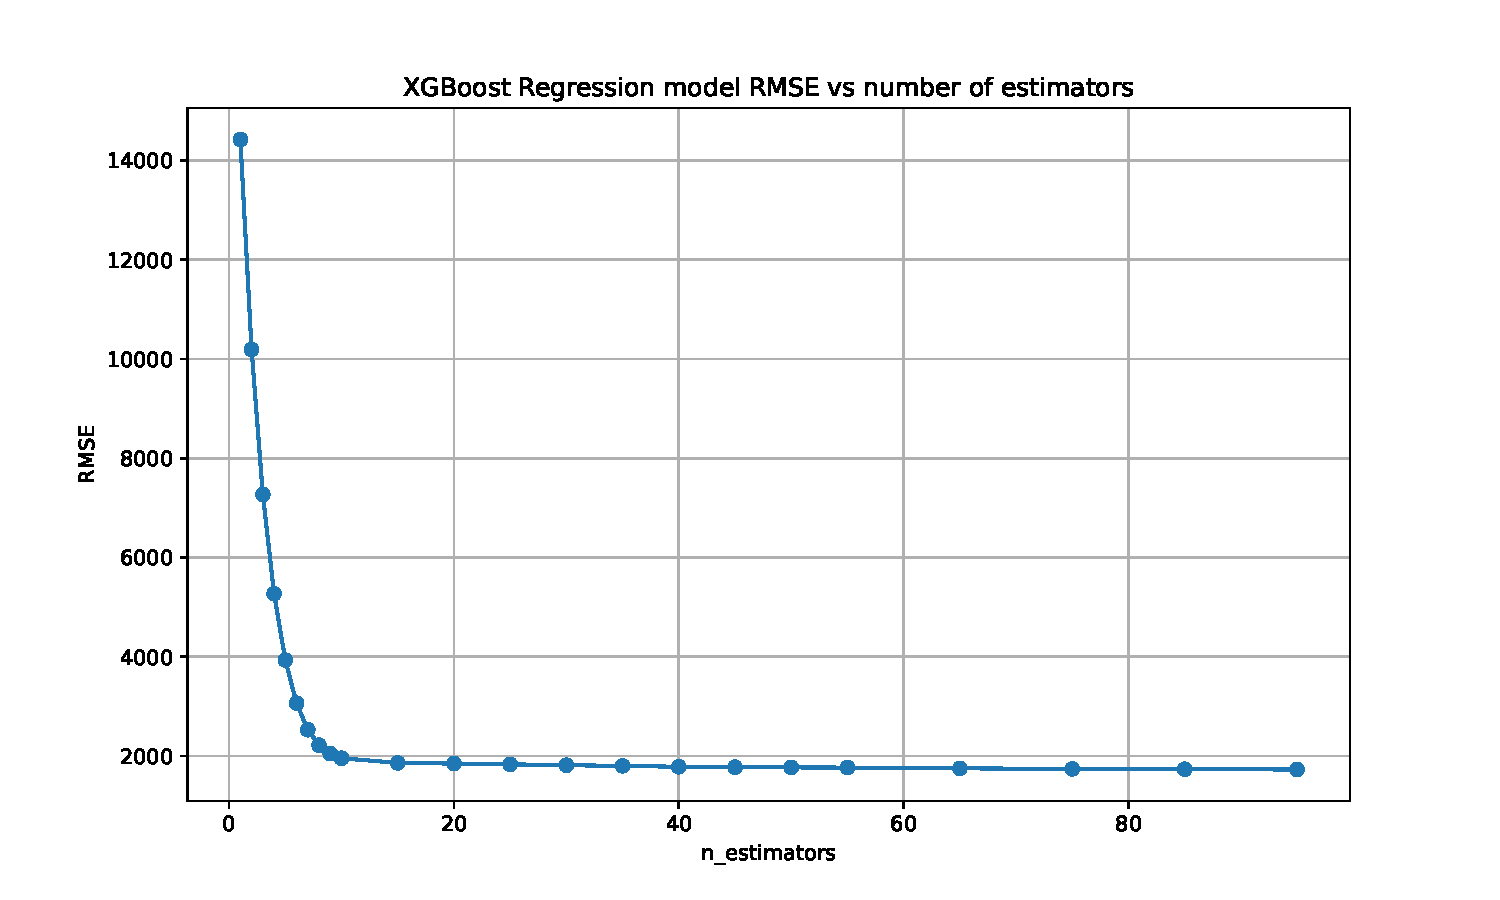
\includegraphics[width=\textwidth]{../regression_model/plots/XGB/XGBoost Regression model RMSE vs n_estimators.pdf}
        \caption{RMSE vs number of estimators}
        \label{fig: XGBoost N estimators vs RMSE}
    \end{subfigure}
    \caption[XGBoost metric results]{XGBoost regression model results plots}
    \label{fig: XGBoost estimators vs results}
\end{figure}
% Comparison plots
\begin{figure}[!htbp]
    \centering
    \begin{subfigure}[b]{0.49\textwidth}
        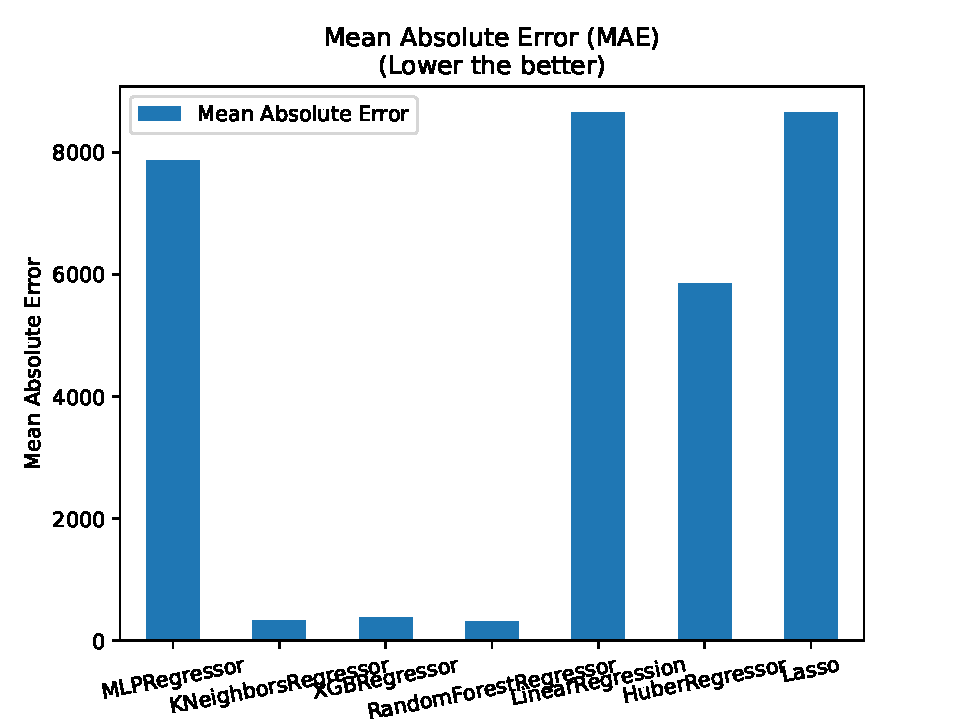
\includegraphics[width=\textwidth]{../regression_model/plots/Comparison/Mean_Absolute_Error.pdf}
        \caption{All regressor model mean absolute error results (lower the better)}
        \label{Fig: all_MAE}
    \end{subfigure}
    \hfill
    \begin{subfigure}[b]{0.49\textwidth}
        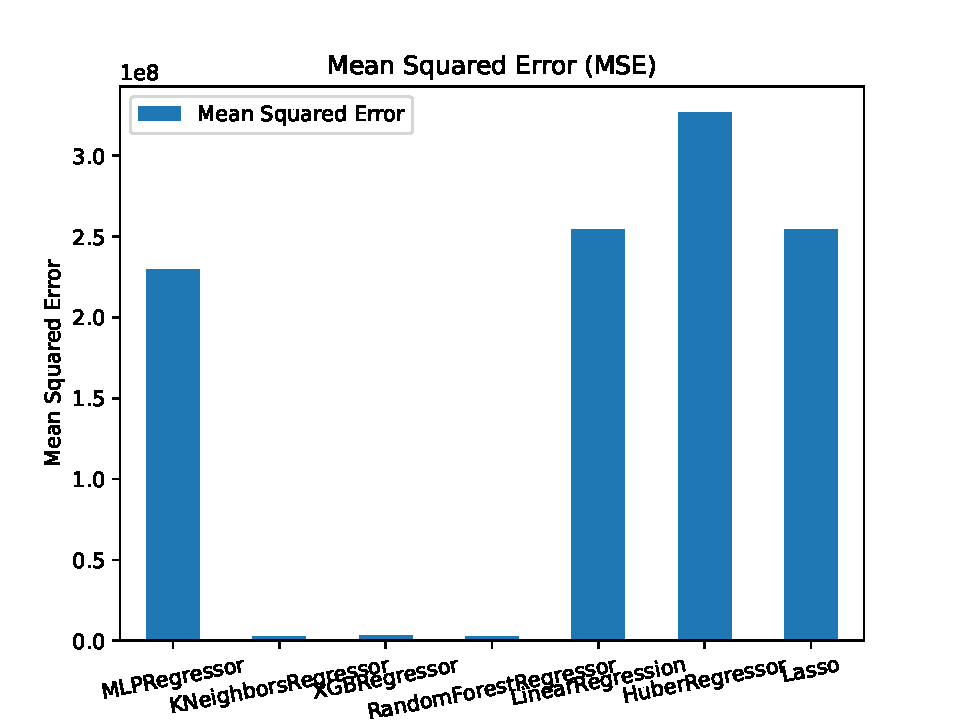
\includegraphics[width=\textwidth]{../regression_model/plots/Comparison/Mean_Squared_Error.pdf}
        \caption{All regressor model squared absolute error results (lower the better)}
        \label{Fig: all_MSAE}
    \end{subfigure}
    \vskip\baselineskip
    \begin{subfigure}[b]{0.49\textwidth}
        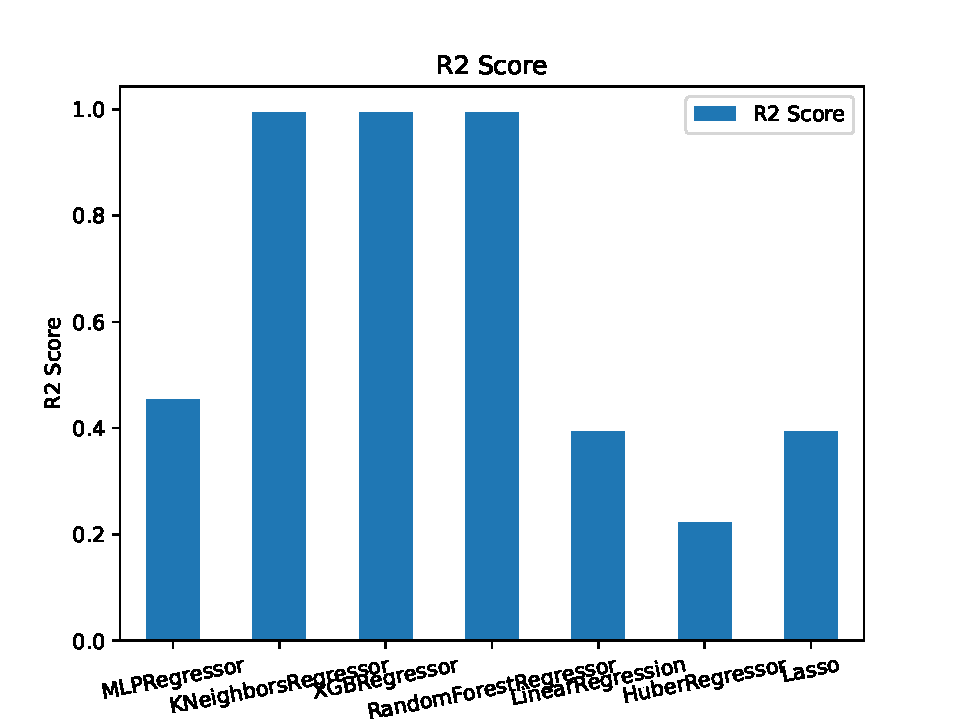
\includegraphics[width=\textwidth]{../regression_model/plots/Comparison/R2_Score.pdf}
        \caption{All regressor model $R^2$ results}
        \label{Fig: all_R2}
    \end{subfigure}
    \hfill
    \begin{subfigure}[b]{0.49\textwidth}
        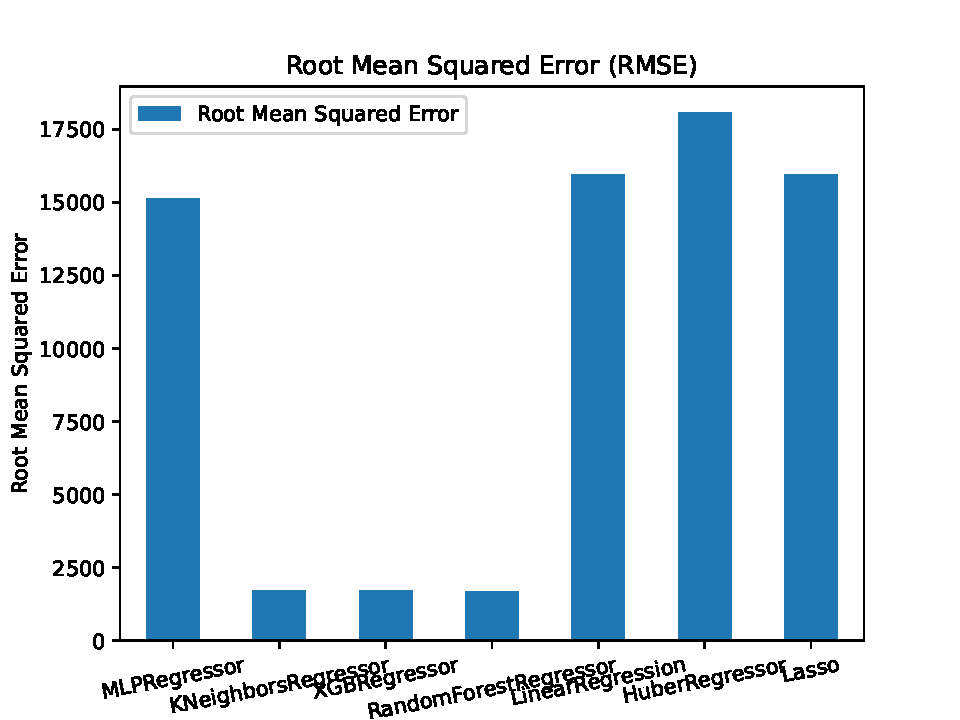
\includegraphics[width=\textwidth]{../regression_model/plots/Comparison/Root_Mean_Squared_Error.pdf}
        \caption{All regressor model root mean squared error results (lower the better)}
        \label{Fig: all_RMSE}
    \end{subfigure}
\end{figure}

% \begin{figure}
%     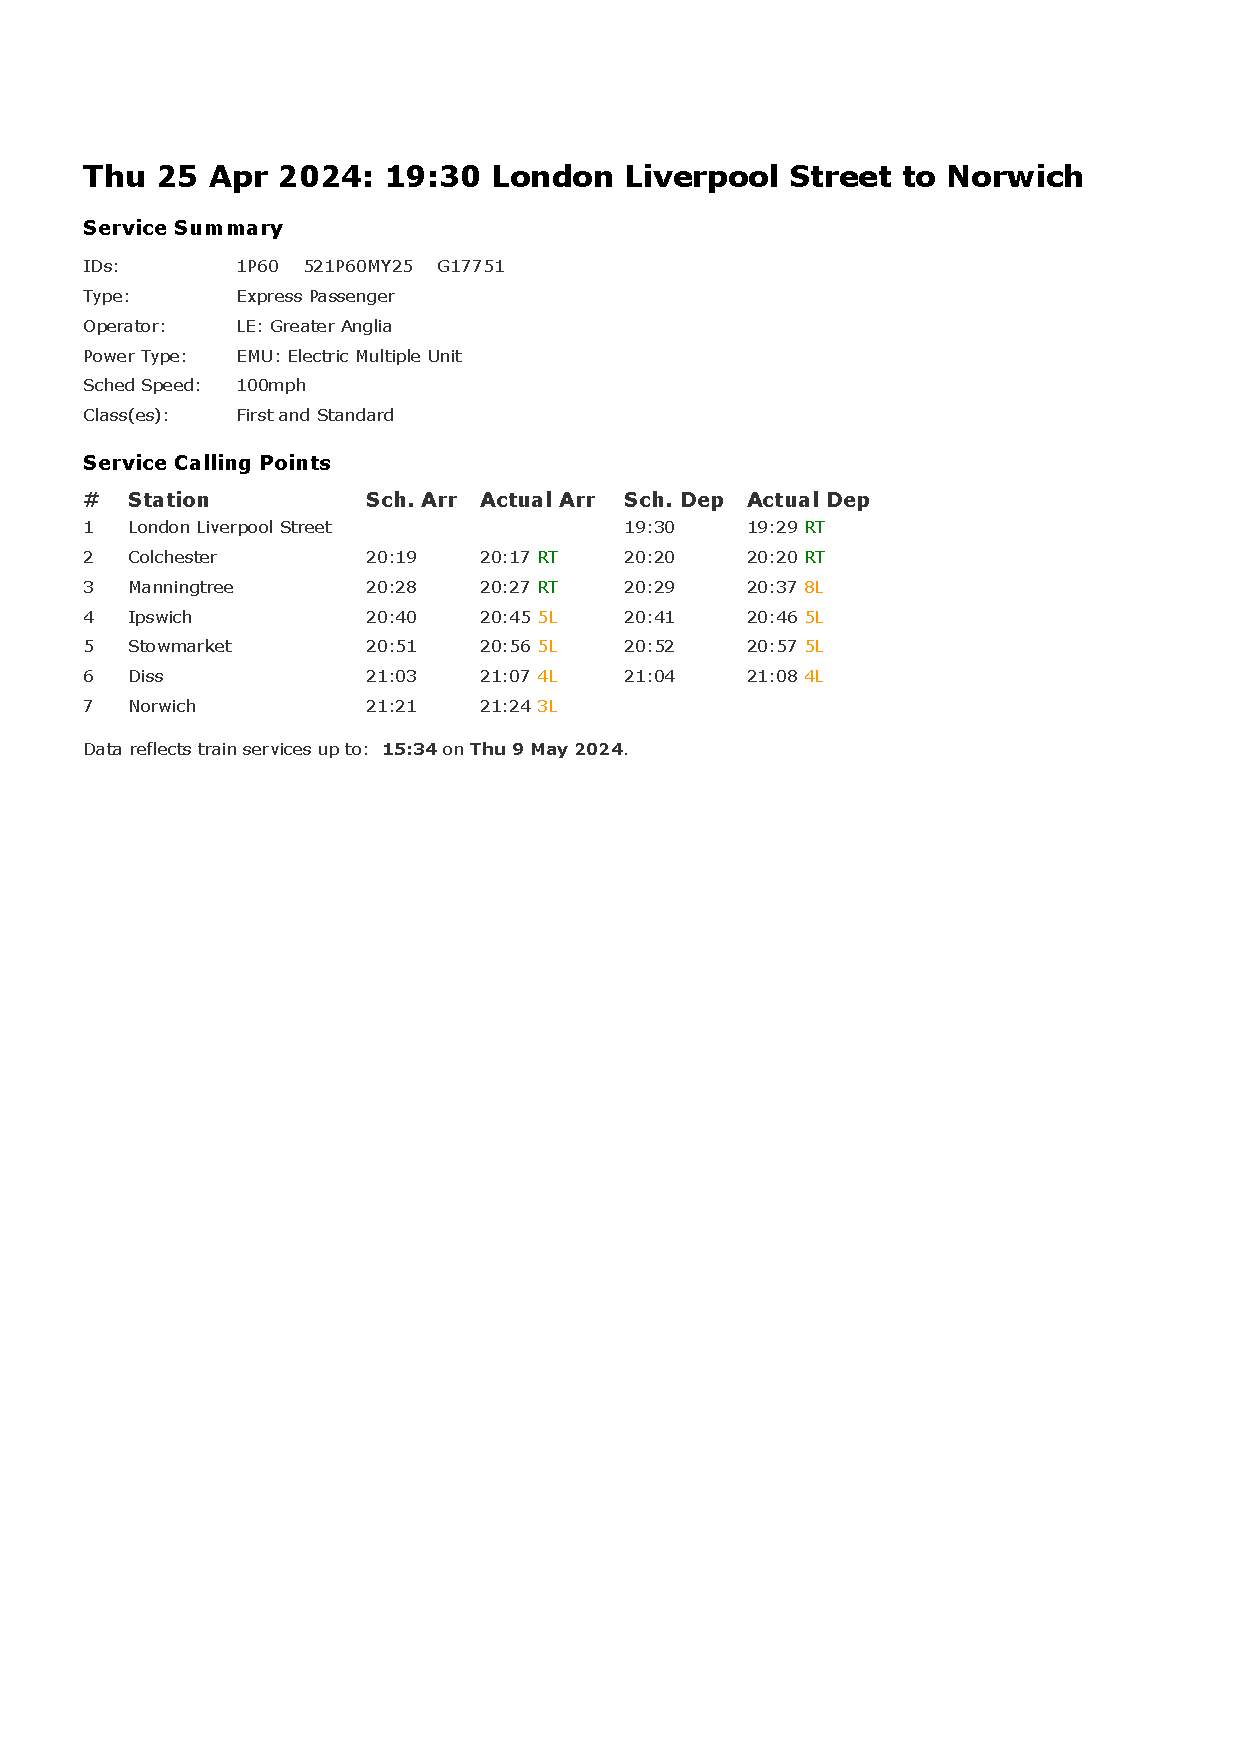
\includegraphics{Diagrams/Exmple of train times/Late/Service Information_25-04-24.pdf}
%     \caption[short]{An eaxmple of a real train journey}
% \end{figure}

\begin{figure}[!htbp]
    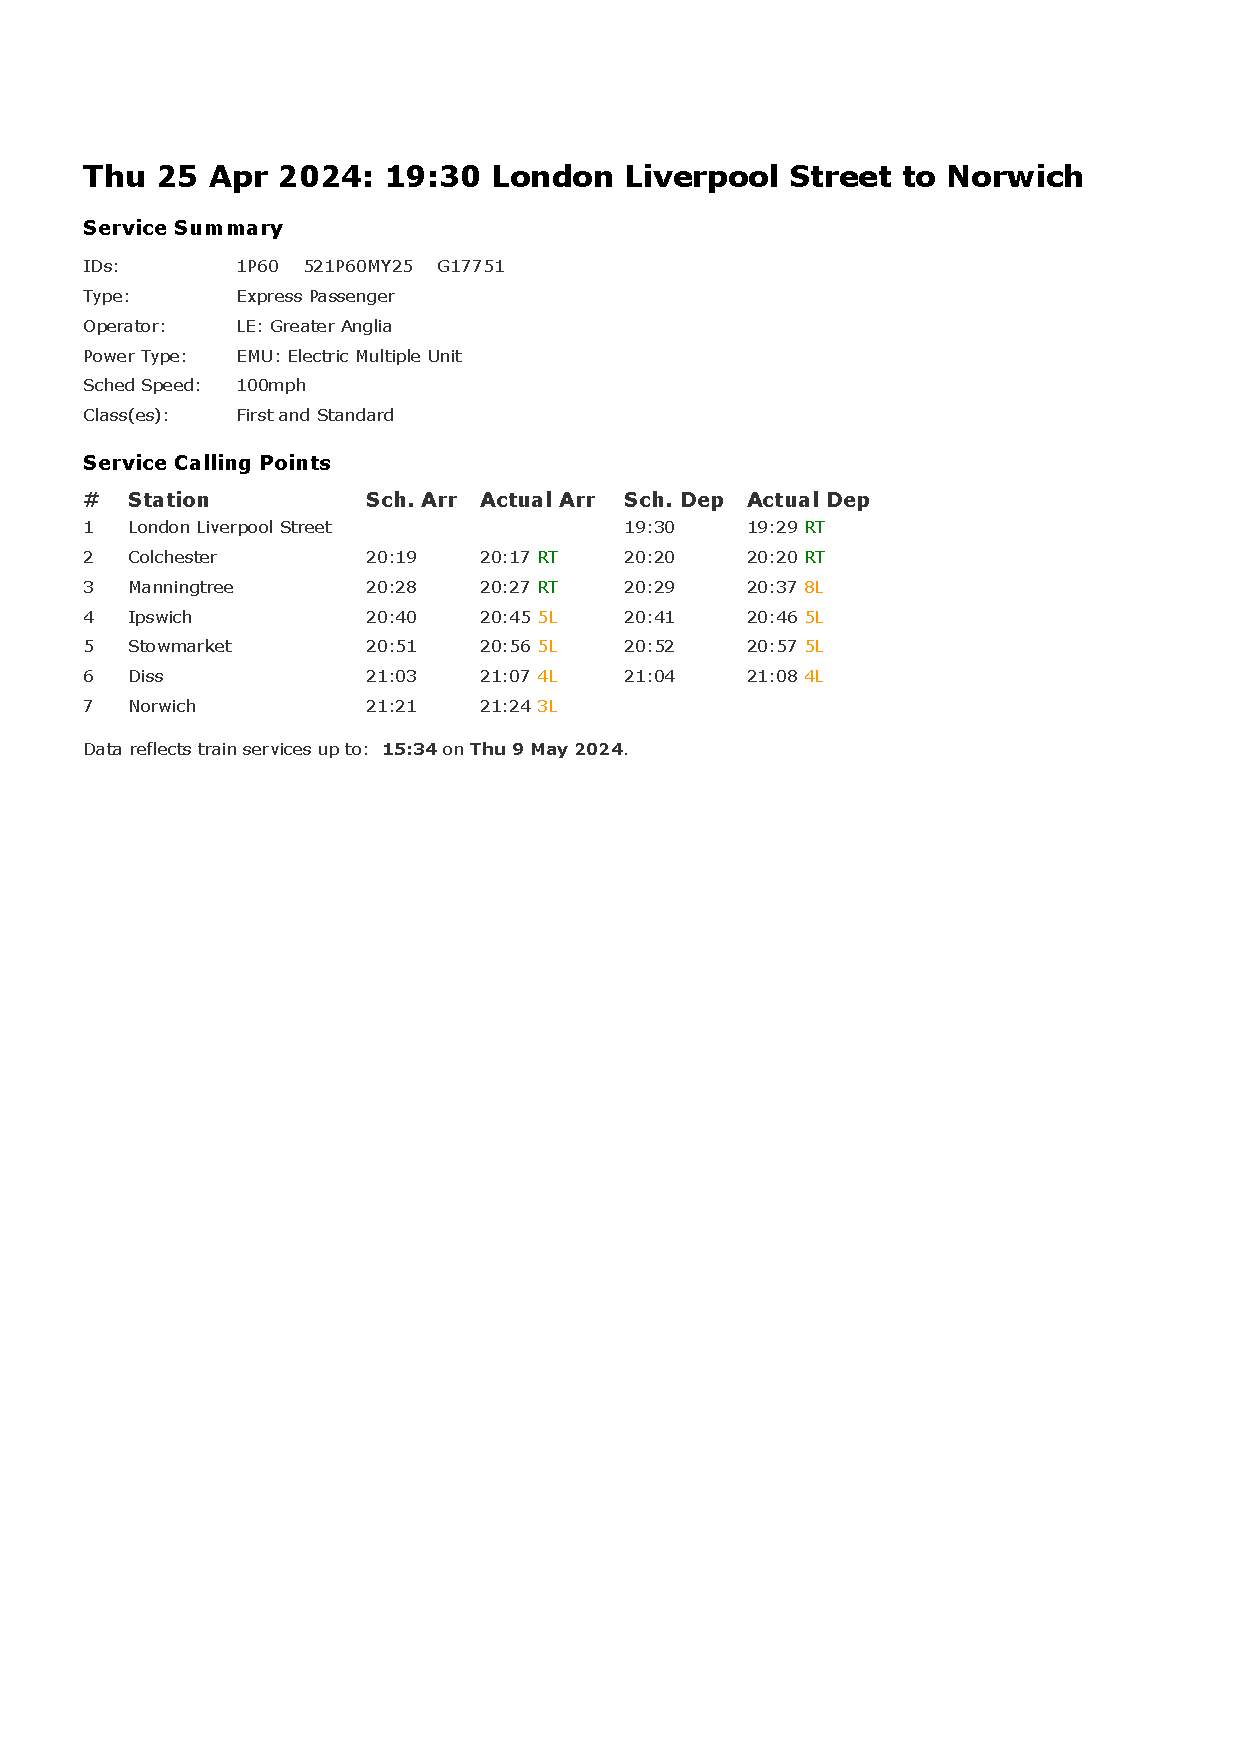
\includegraphics[trim=0 480 0 0]{Diagrams/Exmple of train times/Late/Service Information_25-04-24.pdf}
    \caption[short]{An example of a delayed train journey}
    \label{fig: real delayed train times}
\end{figure}

\begin{figure}[!htbp]
    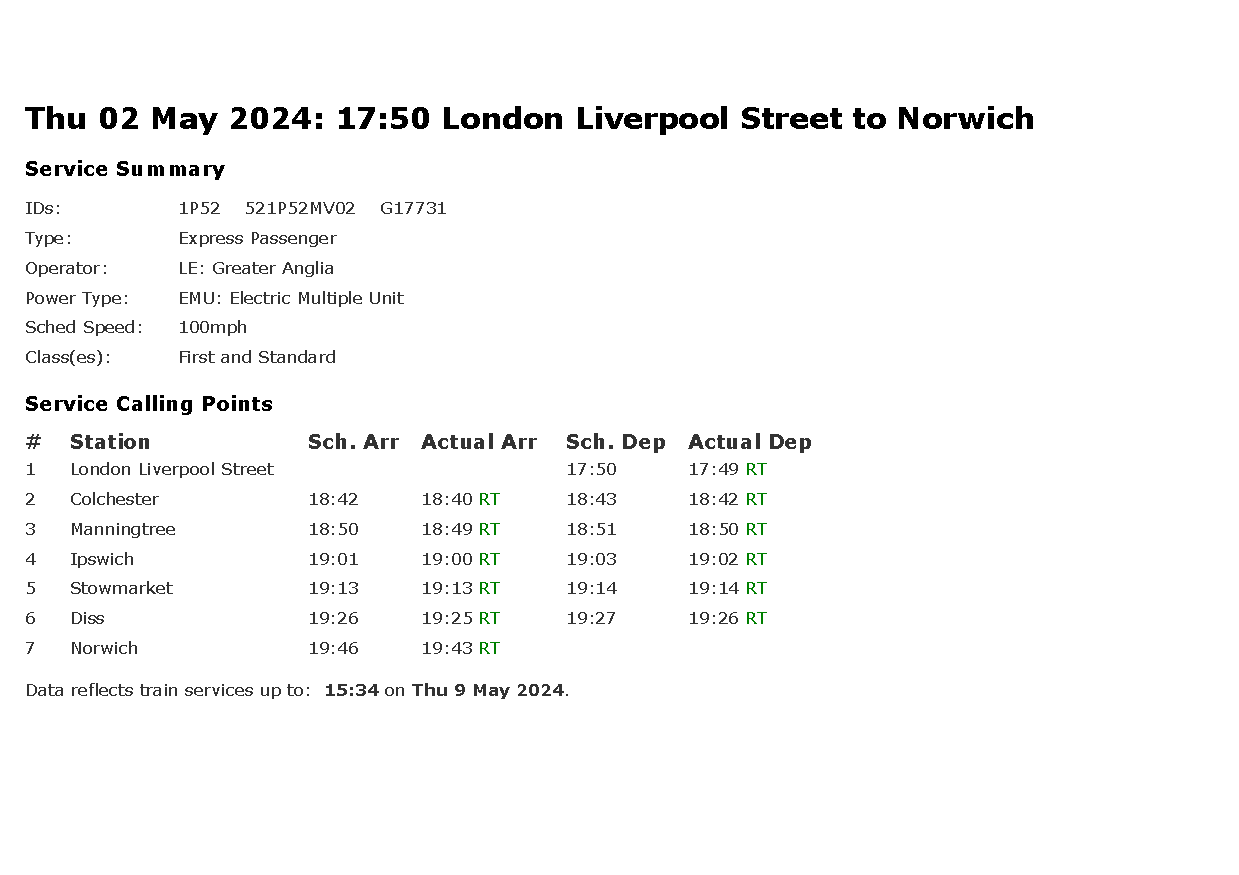
\includegraphics[trim=0 80 0 0]{Diagrams/Exmple of train times/On-Time/Service Information_02-05-24.pdf}
    \caption[short]{An example of an on-time train journey}
    \label{fig: real on-time train times}
\end{figure}

\begin{figure}[!htbp]
    \centering
    \begin{subfigure}[b]{\textwidth}
        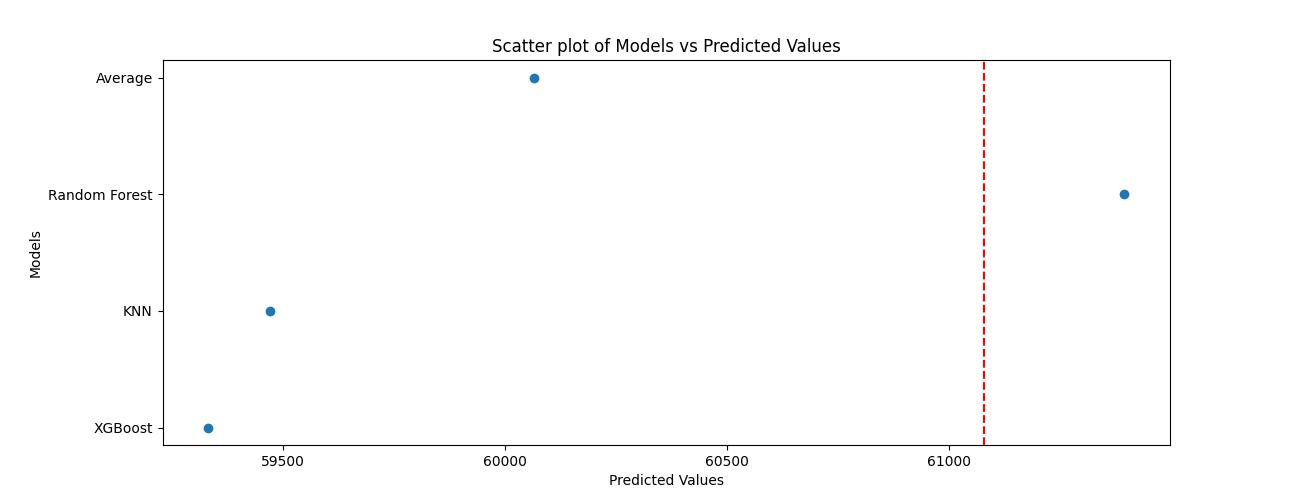
\includegraphics[width=\textwidth]{../regression_model/plots/Comparison/Scatter plot of Models vs Predicted Value 61080.jpeg}
        \caption[short]{}
        \label{}
    \end{subfigure}
    \par
    \begin{subfigure}[b]{\textwidth}
        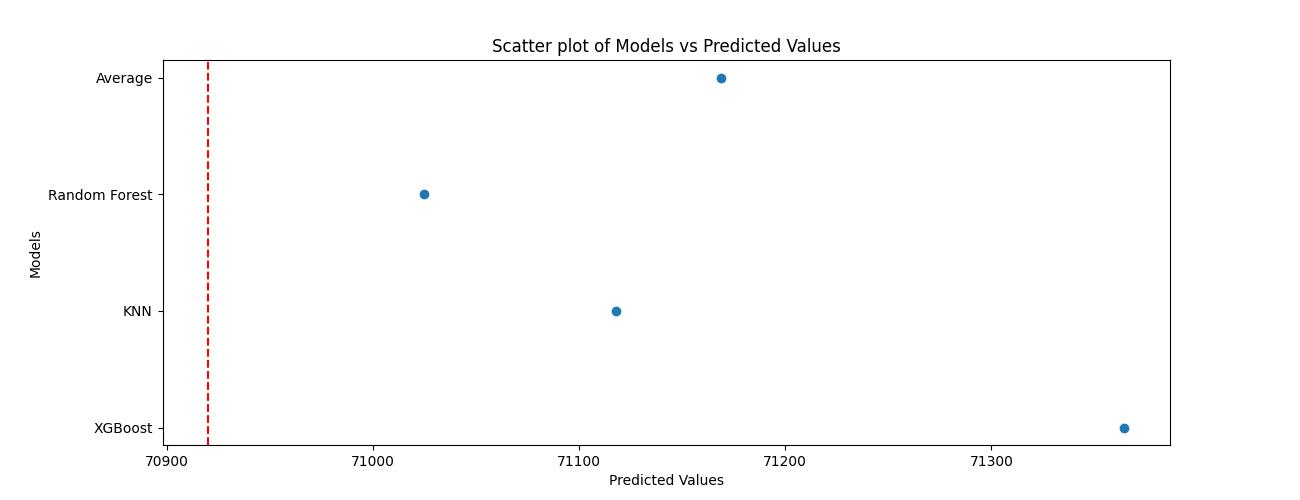
\includegraphics[width=\textwidth]{../regression_model/plots/Comparison/Scatter plot of Models vs Predicted Value 70920.jpeg}
        \caption[short]{}
        \label{}
    \end{subfigure}
    \par
    % \vskip\baselineskip
    \begin{subfigure}[b]{\textwidth}
        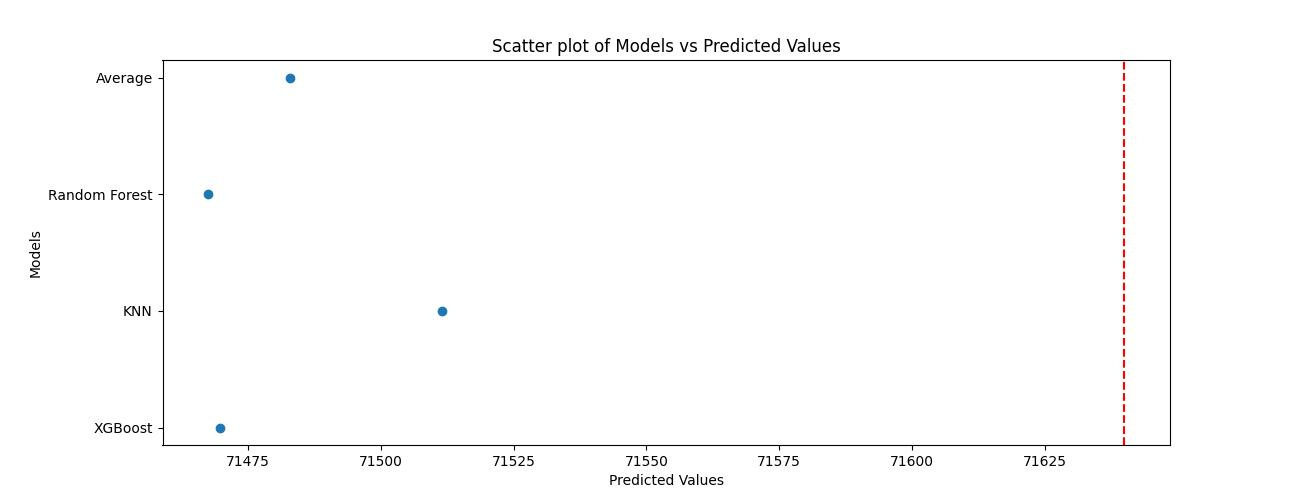
\includegraphics[width=\textwidth]{../regression_model/plots/Comparison/Scatter plot of Models vs Predicted Value 71640.jpeg}
        \caption[short]{}
        \label{}
    \end{subfigure}
    \caption[short]{Regression model predicted arrival time at Norwich from London Liverpool Street if delayed at Ipswich. The red dotted vertical line is ground truth.}
    \label{fig: Regression model predicted arrival time at Norwich from London Liverpool Street}
\end{figure}

\begin{figure}[!htbp]
    \centering
    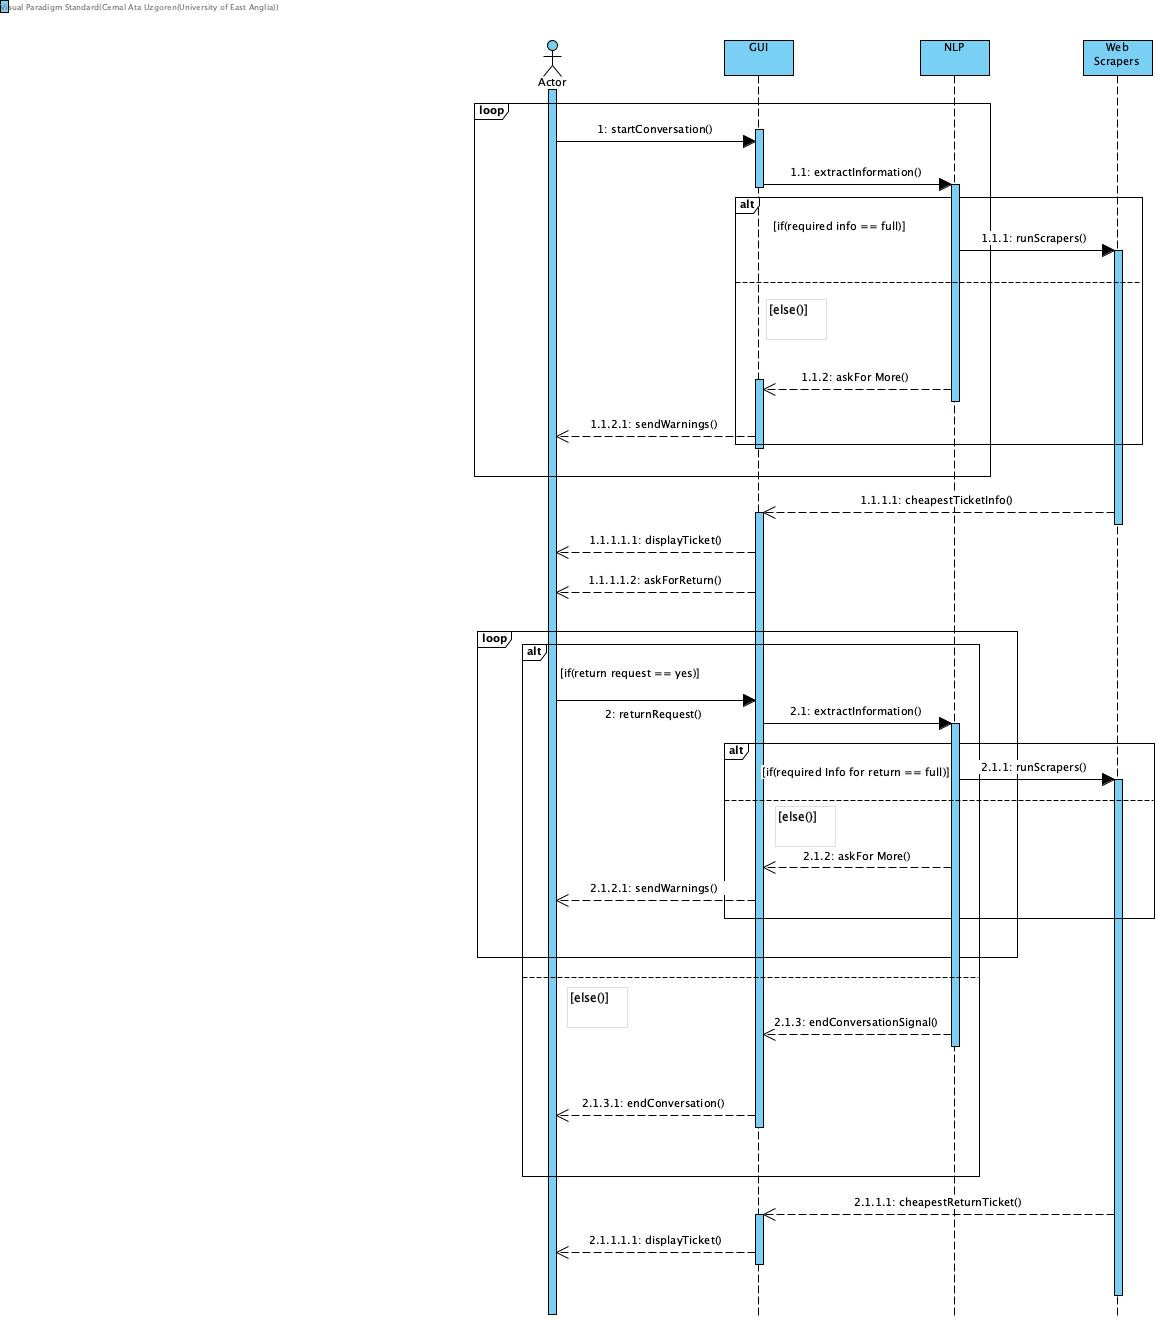
\includegraphics[trim= 350 0 0 0,width= 0.8\textwidth]{Diagrams/ata_diags/Sequence Diagram of Part-1.jpg}
    \caption{A sequence diagram for the chatbot's ticket scraping mechanism}
    \label{Fig: seq diag ticket scraping}
\end{figure}

\begin{figure}[!htbp]
    \centering
    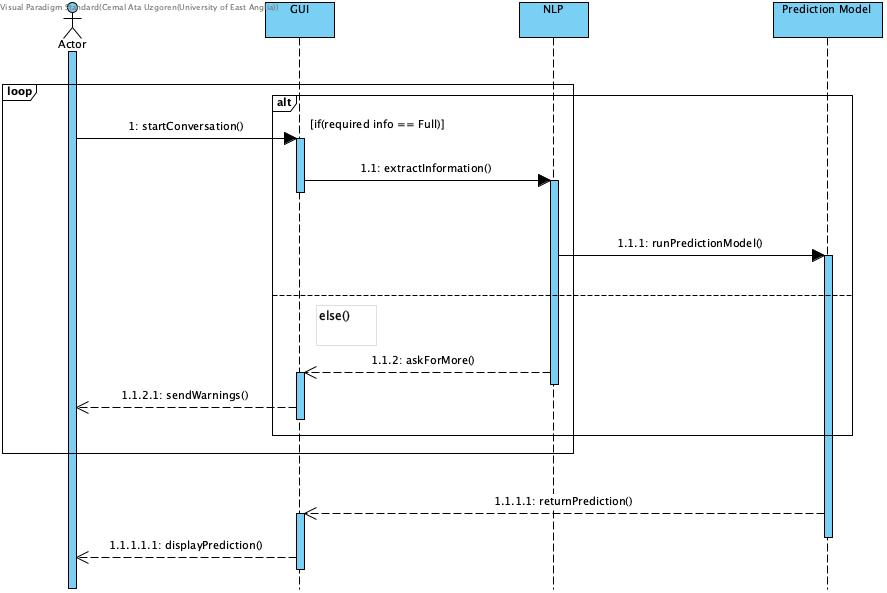
\includegraphics[width= 0.8\textwidth]{Diagrams/ata_diags/Sequence Diagram of Part-2.jpg}
    \caption{A sequence diagram for the chatbot's delayed journey mechanism}
    \label{Fig: seq diag delay prediction}
\end{figure}

\begin{figure}[!htbp]
    \centering
    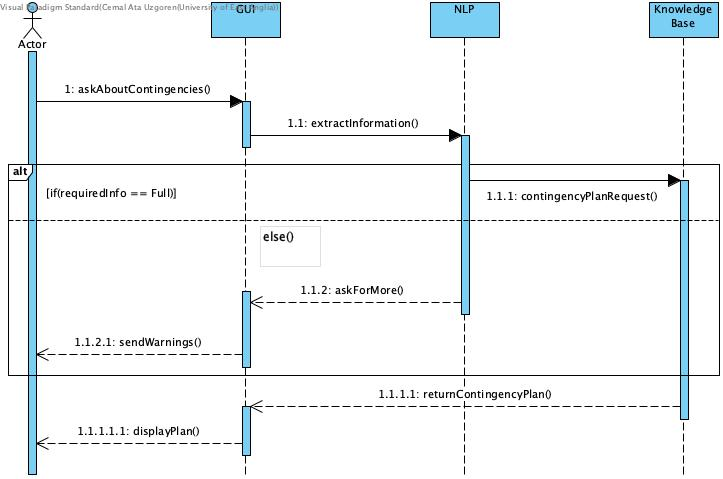
\includegraphics[width= 0.8\textwidth]{Diagrams/ata_diags/Sequence Diagram for Part-3.jpg}
    \caption{A sequence diagram for the chatbot's contingency mechanism}
    \label{Fig: seq diag contingency}
\end{figure}

\begin{figure}[!htbp]
    \centering
    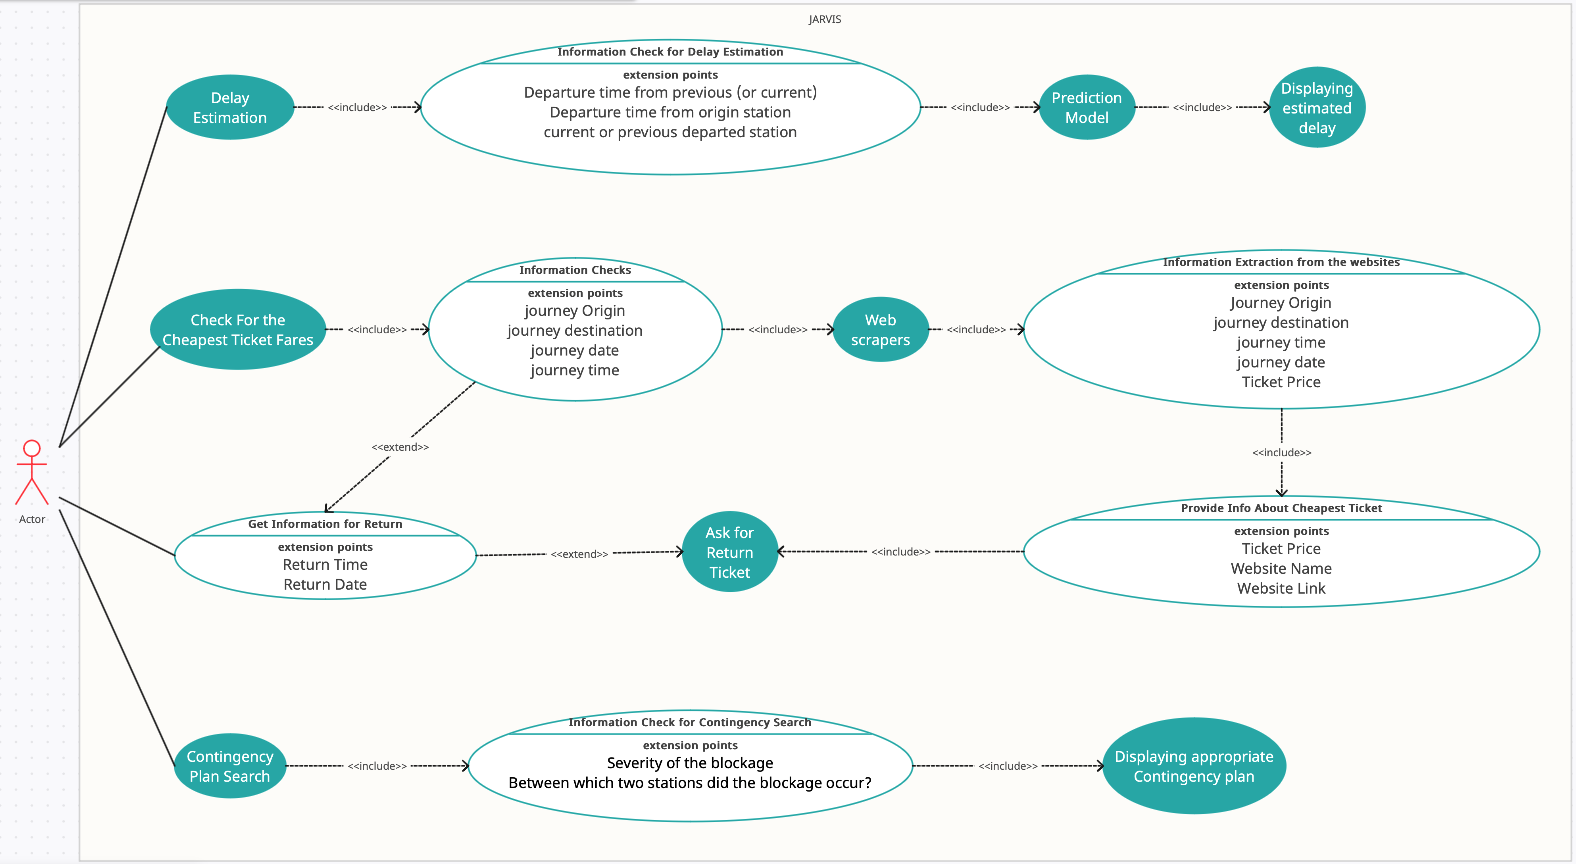
\includegraphics[width=\textwidth]{Diagrams/ata_diags/image.png}
    \caption{A use case diagram for the entire chatbot system}
    \label{Fig: use case whole system}
\end{figure}

\begin{figure}[!htbp]
    \centering
    % 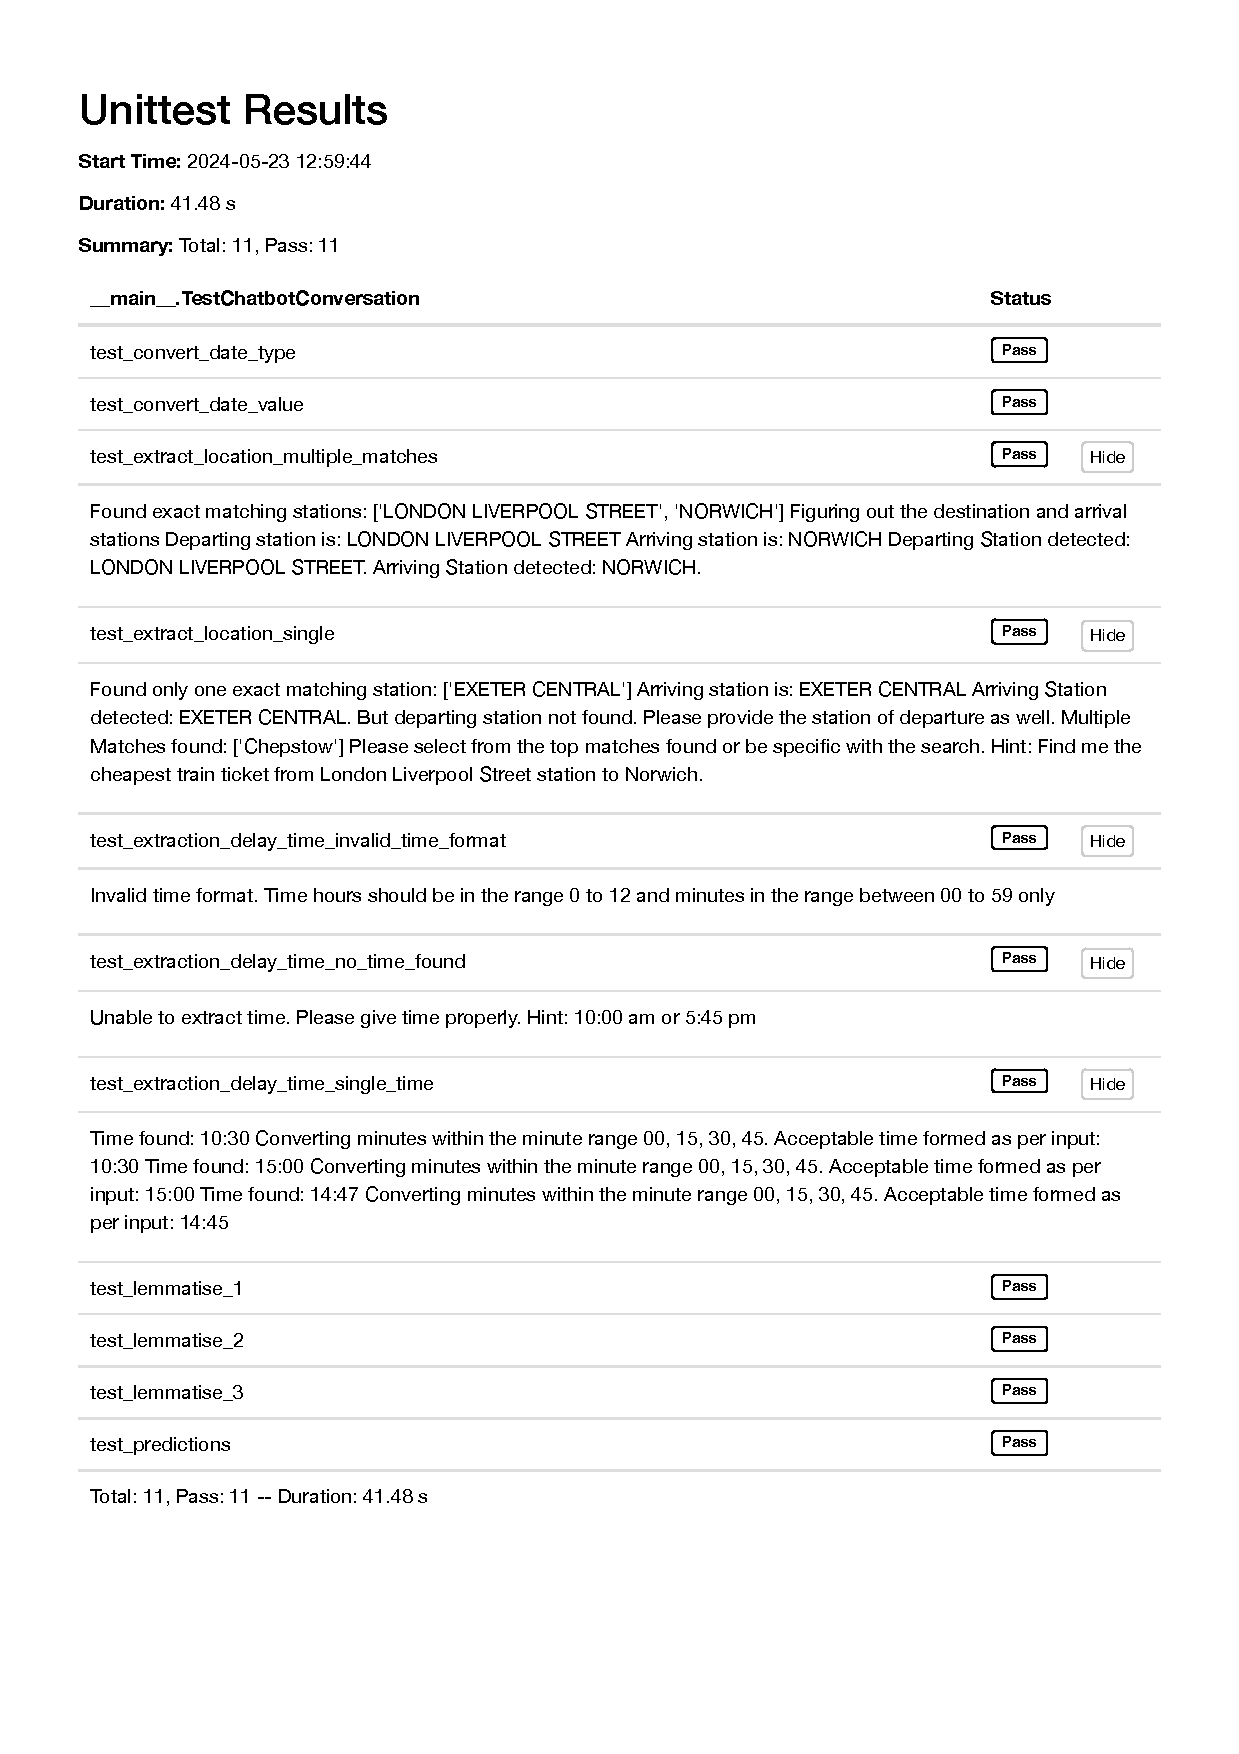
\includegraphics[trim = 0 100 0 0, width=\textwidth]{Diagrams/Unit_Test_HTML/Unittest Results.pdf}
    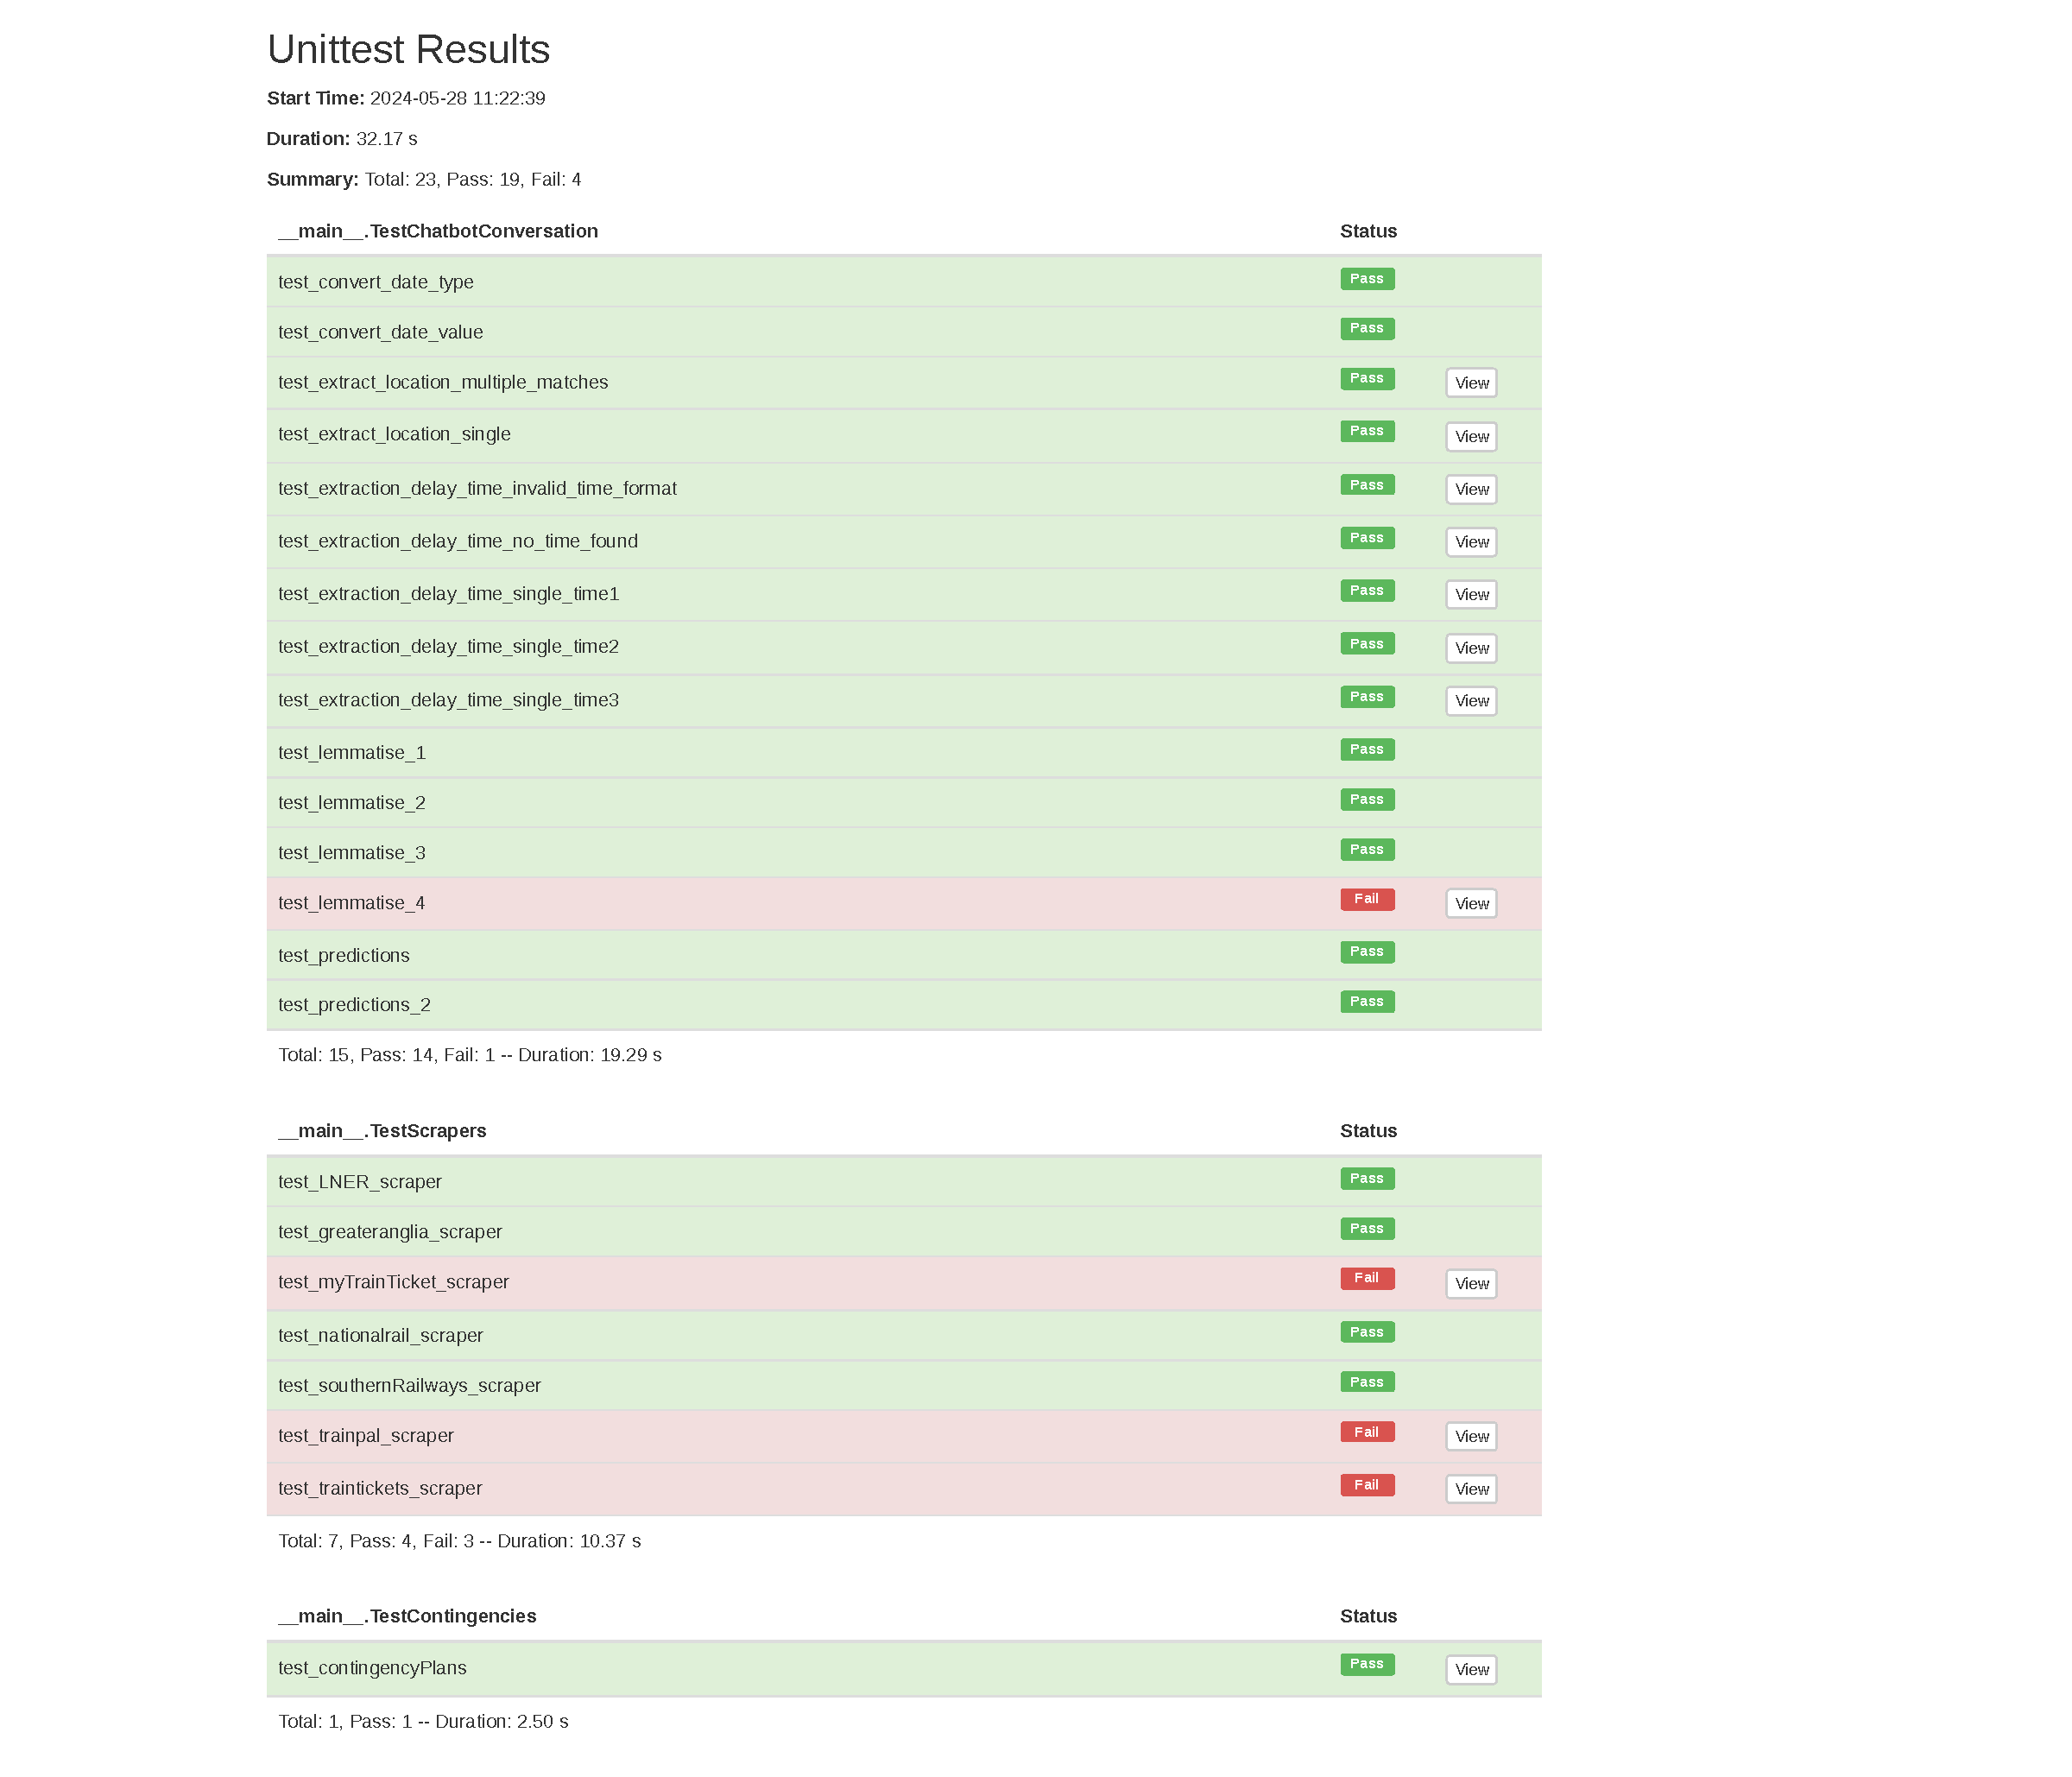
\includegraphics[width=1.2\textwidth]{../Tests/TestResults_TestChatbotConversation_TestScrapers_TestContingencies_2024-05-28_11-22-39.pdf}
    \caption{Results from the unit tests executed during the development of the chatbot}
    \label{Fig: unit test results}
\end{figure}

\clearpage
\subsection{Group Work}
\begin{table}[H]
    \centering
    \begin{tabular}{|l|c|}
        \hline
        \textbf{Team Member} & \textbf{Contribution (\%)} \\
        \hline
        Cemal Ata Uzgoren & 33.33\% \\
        \hline
        Aman Seth & 33.33\% \\
        \hline
        Joshua Newton & 33.33\% \\
        \hline
    \end{tabular}
    \caption{Team Members and their Contributions}
    \label{tab:team_contributions}
\end{table}

\subsubsection{Trello}
Link of the Trello page: \url{https://trello.com/b/CipZLfxi/cmp-7028b-assignment-02}

\begin{figure}[!htbp]
    \centering
    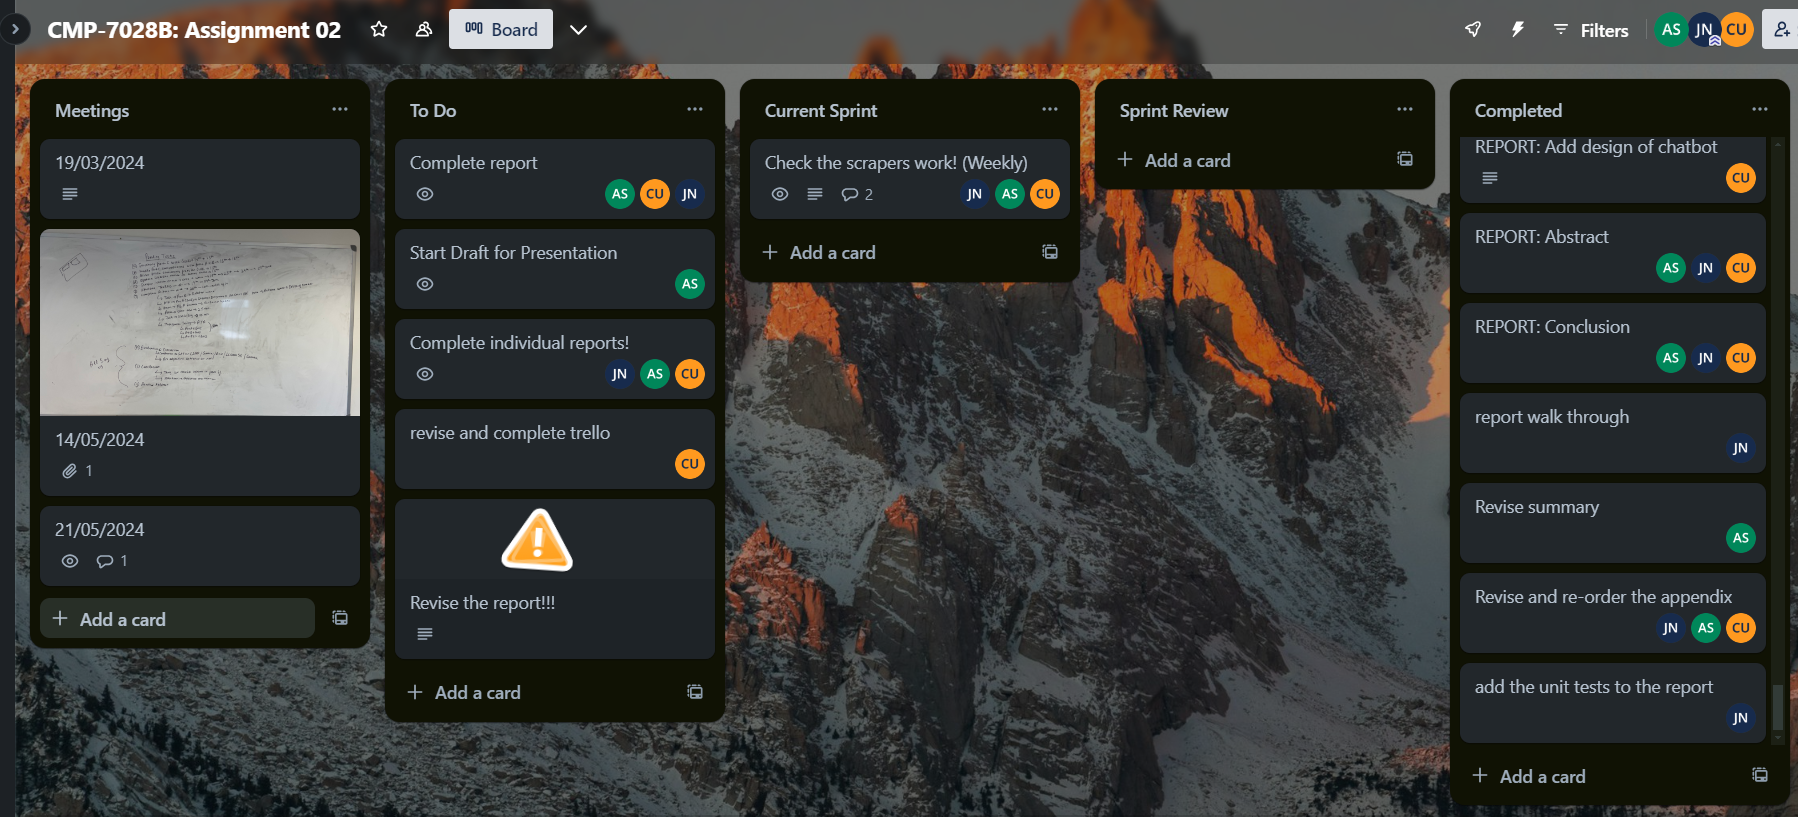
\includegraphics[width=1\linewidth]{Diagrams/Group_work/trello_board.png}
    \caption{Trello Board}
    \label{Fig: trello_ss}
\end{figure}

\begin{figure}[!htbp]
    \centering
    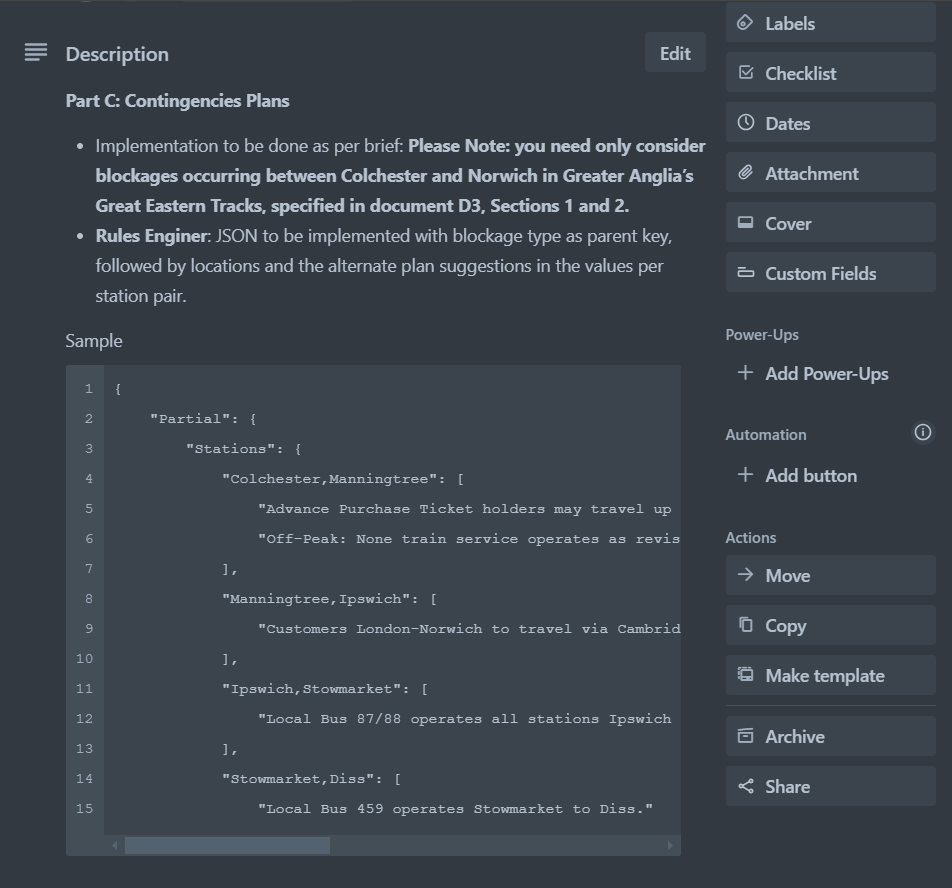
\includegraphics[width=1\linewidth]{Diagrams/Group_work/trello_card.png}
    \caption{Trello Card - Part C}
    \label{Fig: trello_card_c}
\end{figure}

\begin{figure}[!htbp]
    \centering
    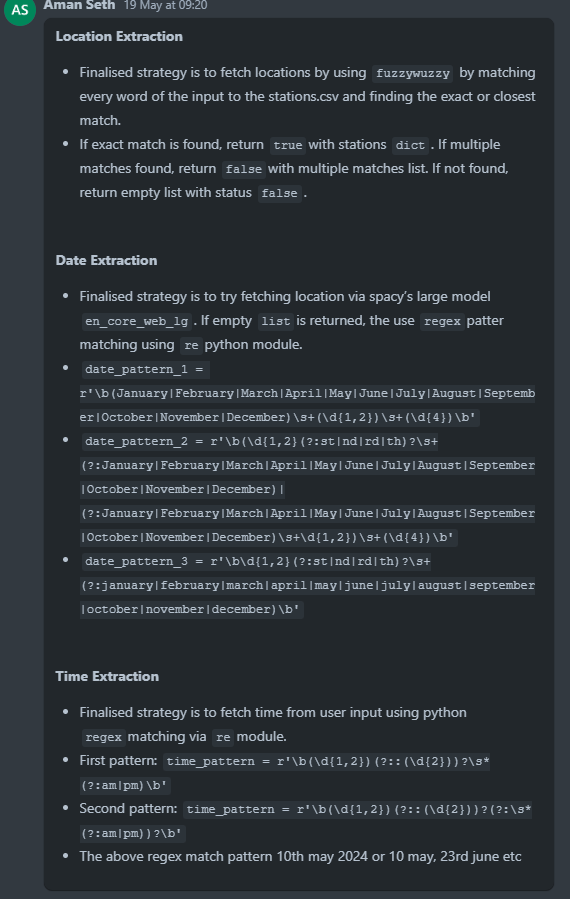
\includegraphics[width=0.8\textwidth]{Diagrams/Group_work/trello_card_2.png}
    \caption{Trello Card - Name Entity Recognition}
    \label{Fig: trello_card_nlp}
\end{figure}

\clearpage
\subsubsection{Github}
Link of the Github page : \url{https://github.com/Staying-Inside/chatbot.git}

\begin{figure}[!htbp]
    \centering
    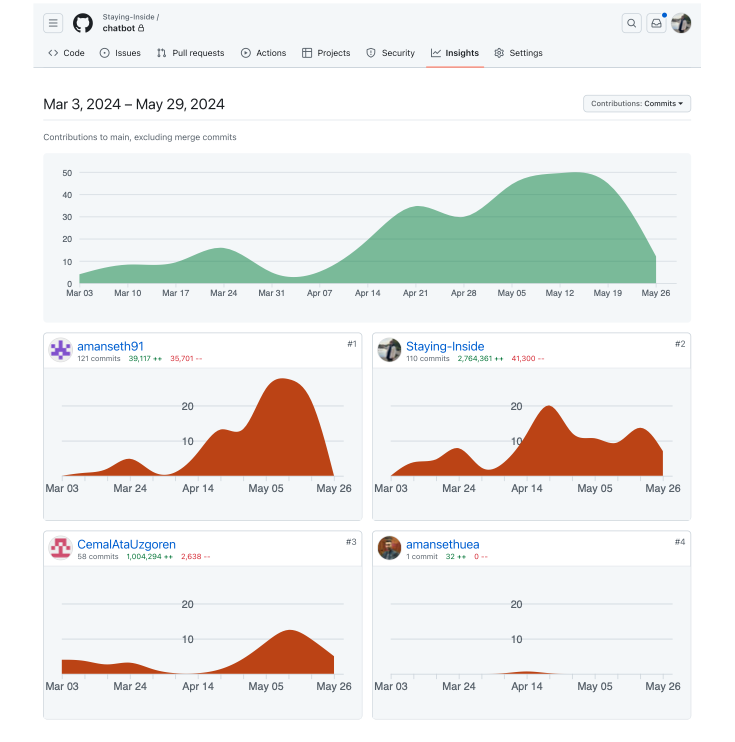
\includegraphics[width=1\linewidth]{Diagrams/Group_work/Github_insights.png}
    \caption{Insights of the project repository}
    \label{fig:insights_github}
\end{figure}

\clearpage

\begin{figure}[!htbp]
    \centering
    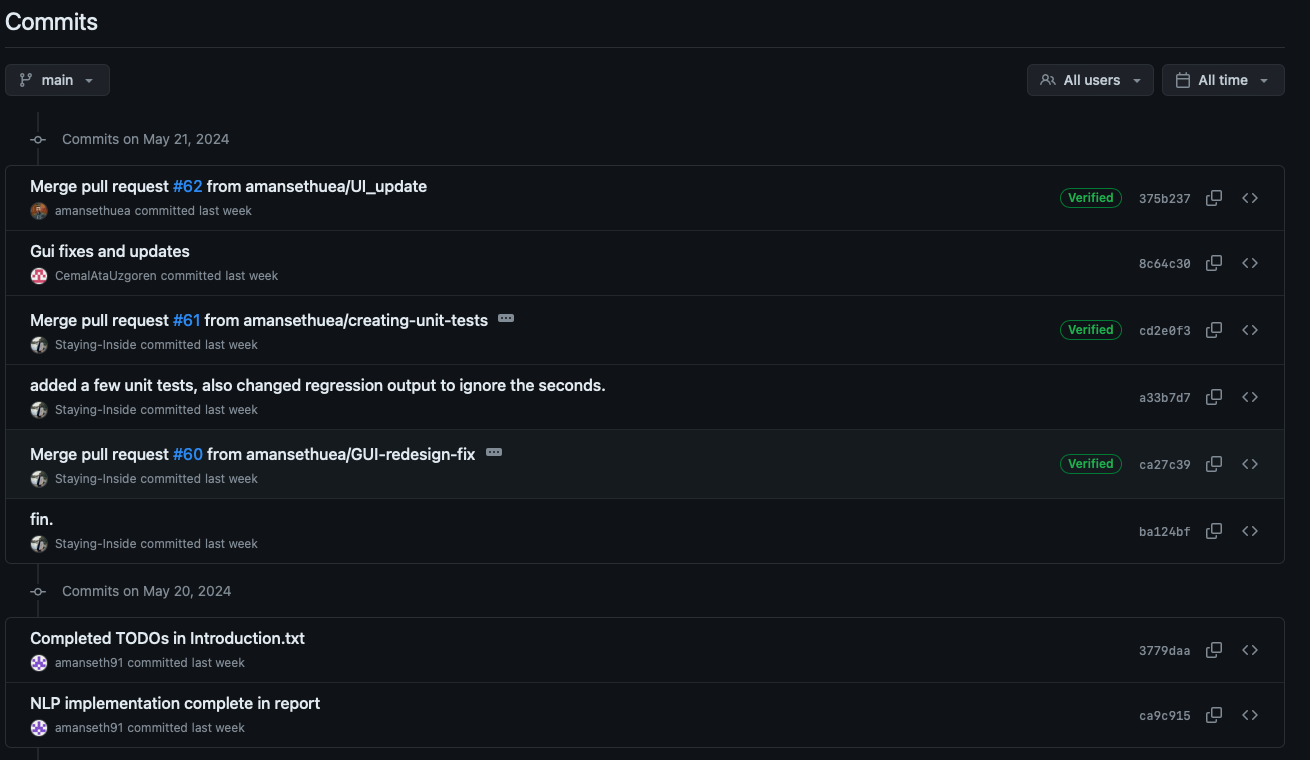
\includegraphics[width=1\linewidth]{Diagrams/Group_work/Github_commit_page.png}
    \caption{Commit screen of the project repository}
    \label{fig:commit_github}
\end{figure}

\clearpage

\subsubsection{Design phase}
\begin{figure}[!htbp]
    \centering
    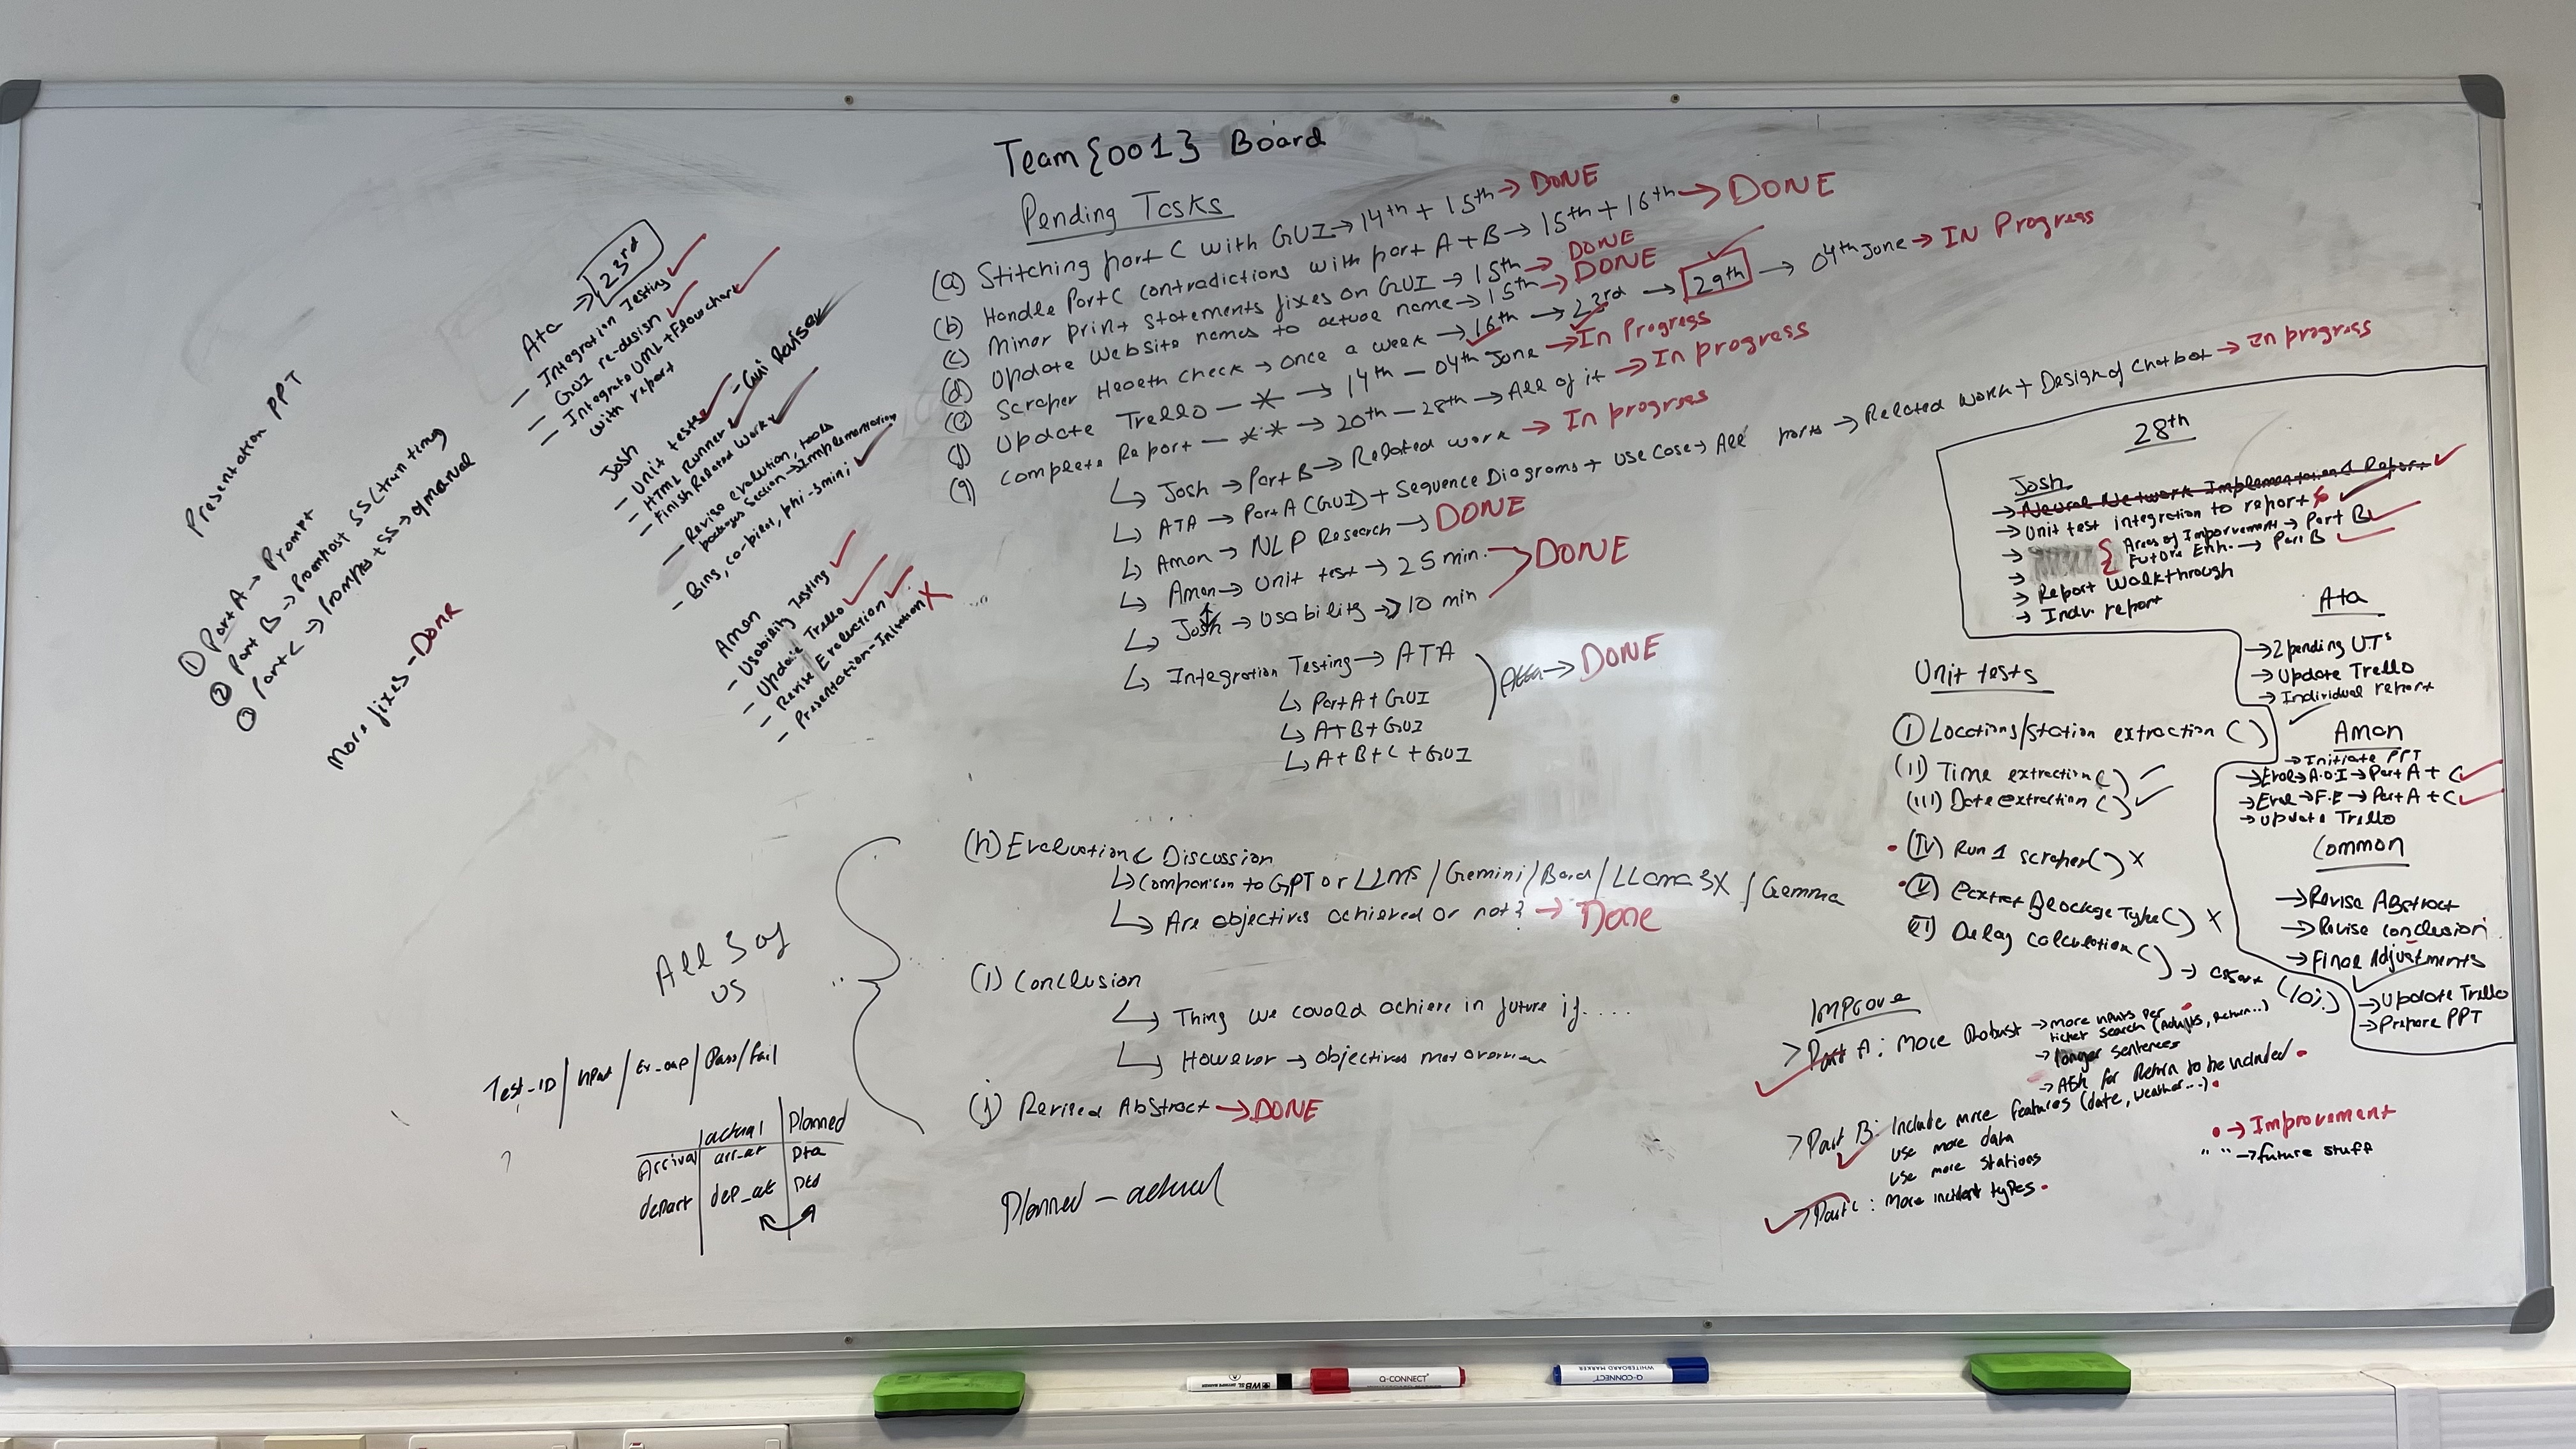
\includegraphics[width=1\linewidth]{Diagrams/Group_work/Group_whiteboard.jpg}
    \caption{Work-load distribution for reporting}
    \label{fig:lab2}
\end{figure}

\begin{figure} [!htbp]
    \centering
    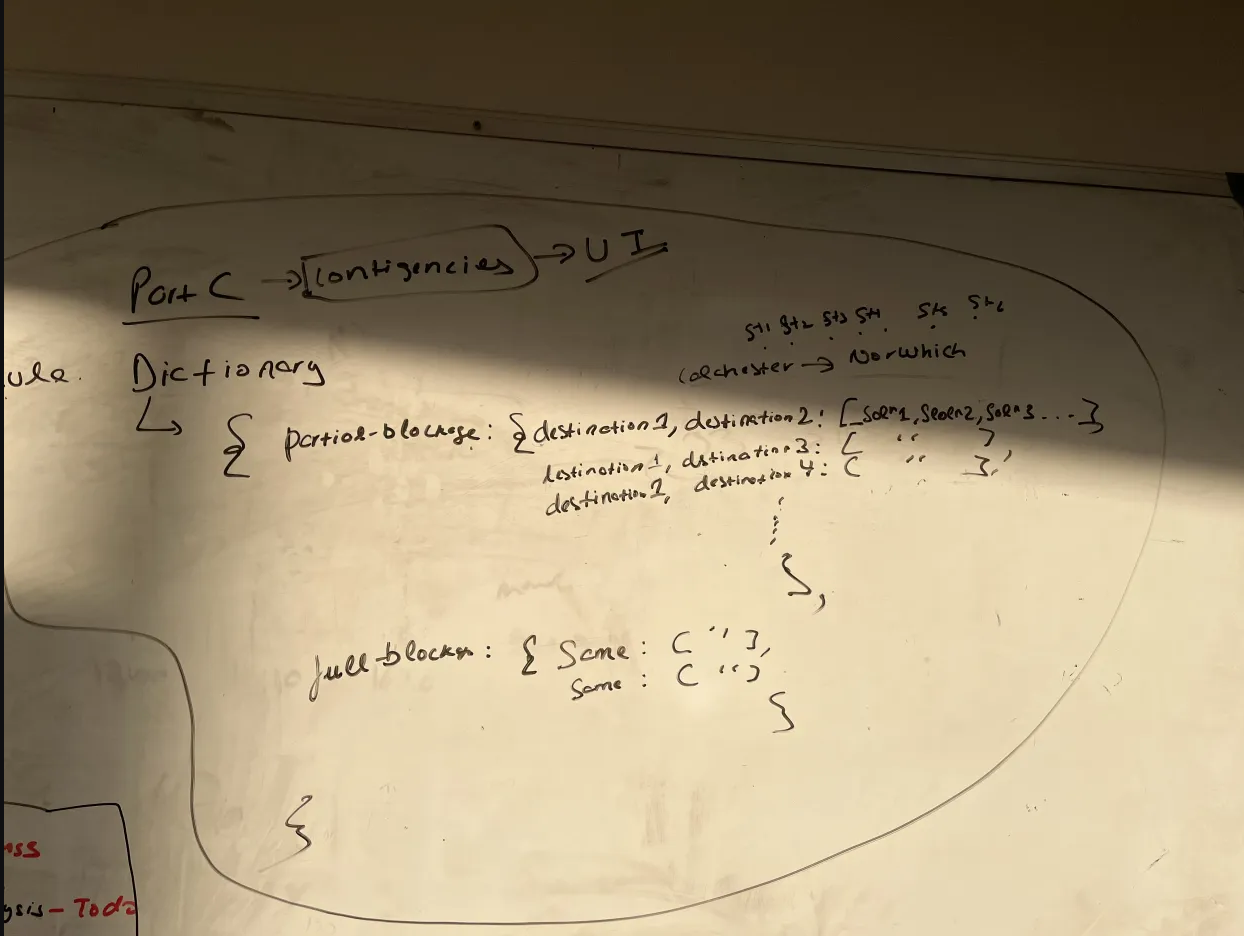
\includegraphics[width=1\linewidth]{Diagrams/Group_work/lab_Handwritings.png}
    \caption{Part-3 plan}
    \label{fig:lab1}
\end{figure}

\clearpage
\subsubsection{Coding Phase}
\textbf{Spawning Python via JS (GUI)}
\begin{figure} [!htbp]
    \centering
    \includegraphics[width=1\linewidth]{Diagrams/Group_work/spawn.png}
    \caption{Code: Spawning Python NLP code via JS}
    \label{fig:python_spawn}
\end{figure}

\textbf{NLP - Date Extraction}
\begin{figure} [!htbp]
    \centering
    \includegraphics[width=1\linewidth]{Diagrams/Group_work/date_extraction_nlp.png}
    \caption{Code: Date Extraction Mechanism}
    \label{fig:date_extraction_nlp}
\end{figure}

\textbf{Prediction Model}
\begin{figure} [!htbp]
    \centering
    \includegraphics[width=1\linewidth]{Diagrams/Group_work/model_loading_code.png}
    \caption{Code: Model Prediction for Part B}
    \label{fig:model_prediction}
\end{figure}

\textbf{Blockage Type Extraction}
\begin{figure} [!htbp]
    \centering
    \includegraphics[width=1\linewidth]{Diagrams/Group_work/part_c.png}
    \caption{Code: Blockage Type Extraction in Part C}
    \label{fig:part_c_blockage}
\end{figure}

\clearpage
\subsubsection{Testing Phase}
\textbf{Testing Scenario: Part A and B integrity constraint}
The below tests demonstrate that the user cannot directly switch conversation to part B (Delay prediction) if there is an on-going conversation regarding part A (Cheapest train fare search) in place. The user may or may not reset the search explicitly in order to proceed.
\begin{figure} [!htbp]
    \centering
    \includegraphics[width=1\linewidth]{Diagrams/Group_work/testing_1.png}
    \caption{Test: Part A and B Integrity Constraint Check}
    \label{fig:test_1}
\end{figure}

\clearpage
\textbf{Testing Scenario: Part B and A integrity constraint}
The below tests demonstrate that the user cannot directly switch conversation to part A (Cheapest train fare search) if there is an on-going conversation regarding part B (Delay prediction) in place. The user may or may not reset the search explicitly in order to proceed.
\begin{figure} [!htbp]
    \centering
    \includegraphics[width=1\linewidth]{Diagrams/Group_work/testing_2.png}
    \caption{Test: Part B and A Integrity Constraint Check}
    \label{fig:test_2}
\end{figure}

\end{document}



% Josh
% TODO: proof read regression parts of report (do all report if i have time)
